\documentclass[jair,twoside,11pt,theapa]{article}
\usepackage{jair, theapa, rawfonts}

\jairheading{70}{2021}{923--954}{09/2020}{03/2021}
\ShortHeadings{Safe Multi-Agent Pathfinding with Time Uncertainty}
{Shahar, Shekhar, Atzmon, Saffidine, Juba, \& Stern}
\firstpageno{923}

%%
\usepackage{amsmath,amssymb,amsthm,amsfonts}
\usepackage{mathtools} % Bonus
\usepackage[noend,ruled,linesnumbered]{algorithm2e}
\usepackage{tikz}
\usepackage{lipsum}
\usepackage{csquotes}
\usepackage{verbatim}
\usepackage{booktabs,array,multirow}
\usepackage{xspace}
\usepackage{caption}
\usepackage{subcaption}
%%
\graphicspath{ {Figures/} }
\SetNlSty{bfseries}{\color{black}}{}


\newcommand{\tuple}[1]{\langle#1\rangle}
\newcommand{\mltr}[1]{\multirow{3}{*}{#1}}
\newcommand{\naturals}{\mathbb{N}}
\newcommand{\graph}{\mathcal{G}}
\newcommand{\vertices}{\mathcal{V}}
\newcommand{\edges}{\mathcal{E}}
\newcommand{\timel}{w^-}
\newcommand{\astar}{A$^*$\xspace}
\newcommand{\timeu}{w^+}
\newcommand{\Cost}{\mathit{Cost}}
\newcommand{\sol}{\mathit{solution}}
\newcommand{\const}{\mathit{constraints}}
\newcommand{\eg}{e.g.,}
%\newcommand{\timeuncertainties}{w}
\newcommand{\sourcetargets}{\mathcal{S}}
\newcommand{\vertexpath}{\pi}
\newcommand{\potential}{\tau}
\newcommand{\oda}{$\mathrm{A^{*}+OD}$\xspace}
%\newcommand{\odatu}{$\mathrm{ODATU}$\xspace}
\newcommand{\odatu}{$\mathrm{A^{*}+OD_{TU}}$\xspace}
\newcommand{\cbstu}{CBS$\mathrm{_{TU}}$\xspace}
\newcommand{\mapftu}{MAPF-TU\xspace}
\newcommand{\sense}{SENSE\xspace}
\newcommand{\sensecom}{SENSE+COM\xspace}
\newcommand{\socopt}{SOC$_{opt}$\xspace}
\newcommand{\socpes}{SOC$_{pes}$\xspace}

\newtheorem{theorem}{Theorem}
\newtheorem{definition}{Definition}
\newtheorem{example}{Example}
\newtheorem{lemma}{Lemma}

\newenvironment{proofo}{\renewcommand{\proofname}{Proof outline}\proof}{\endproof}

\begin{document}

\title{Safe Multi-Agent Pathfinding with Time Uncertainty}


% \author{\name Steven Minton \email minton@ptolemy.arc.nasa.gov \\
%       \name Andy Philips \email philips@ptolemy.arc.nasa.gov \\
%       \addr NASA Ames Research Center, Mail Stop: 244-7,\\
%       Moffett Field, CA  94035 USA
%       \AND
%       \name Mark D. Johnston \email johnston@stsci.edu \\
%       \addr Space Telescope Science Institute,
%       3700 San Martin Drive,\\
%       Baltimore, MD 21218 USA
%       \AND
%       \name Philip Laird \email laird@ptolemy.arc.nasa.gov \\
%       \addr NASA Ames Research Center,
%       AI Research Branch, Mail Stop: 269-2,\\
%       Moffett Field, CA  94035 USA}

\author{\name Tomer Shahar \email stomer@post.bgu.ac.il  \\
        \name Shashank Shekhar \email shekhar@post.bgu.ac.il \\ 
        \name Dor Atzmon \email  dorat@post.bgu.ac.il \\
              \addr Ben-Gurion University of the Negev, Israel
       \AND
       \name Abdallah Saffidine \email abdallah.saffidine@gmail.com \\
       \addr The University of New South Wales, Sydney, Australia
       \AND
       \name Brendan Juba \email bjuba@wustl.edu \\
       \addr Washington University in St.\ Louis, USA
        \AND 
        \name Roni Stern  \\
       \addr Ben-Gurion University of the Negev, Israel \email sternron@post.bgu.ac.il\\
       \addr Palo Alto Research Center, USA \email rstern@parc.com}


% For research notes, remove the comment character in the line below.
% \researchnote

\maketitle


\begin{abstract}
In many real-world scenarios, the time it takes for a mobile agent, e.g., a robot, to move from one location to another may vary due to exogenous events and be difficult to predict accurately. 
Planning in such scenarios is challenging, especially in the context of Multi-Agent Pathfinding (MAPF), where the goal is to find paths to multiple agents and temporal coordination is necessary to avoid collisions. 
In this work, we consider a MAPF problem with this form of time uncertainty, where we are only given upper and lower bounds on the time it takes each agent to move. The objective is to find a \emph{safe} solution, which is a solution that can be executed by all agents and is guaranteed to avoid collisions. 
We propose two complete and optimal algorithms for finding safe solutions
based on well-known MAPF algorithms, namely, \astar with Operator Decomposition (\oda) and Conflict-Based Search (CBS).
Experimentally, we observe that on several standard MAPF grids the CBS-based algorithm performs better. 
We also explore the option of \emph{online} replanning in this context, i.e., modifying the agents' plans during execution, to reduce the overall execution cost. 
We consider two online settings: (a) when an agent can sense the current time and its current location, and (b) when the agents can also communicate seamlessly during execution. 
For each setting, we propose a replanning algorithm and analyze its behavior theoretically and empirically. 
Our experimental evaluation confirms that indeed online replanning in both settings can significantly reduce solution cost.
\end{abstract}


\section{Introduction}
\label{Introduction}

% What is MAPF
Multi-Agent Pathfinding (MAPF) is the problem of finding how to move a team of agents over edges in a graph from an initial configuration to a goal configuration. 
The key constraint is that agents must not occupy the same vertex or traverse the same edge at the same time during plan execution. 
A \emph{solution} to a MAPF problem is a set of \emph{single-agent plans} for all the agents that do not violate this constraint.  % What is a solution to MAPF
MAPF problems arise in real-world applications, such as aircraft towing vehicles \shortcite{MorrisPLMMKK16}, video game characters \shortcite{Silver05}, office robots \shortcite{VelosoBCR15},  %trains \shortcite{AtzmonDR19}, 
and warehouse robots \shortcite{WurmanDM07}. 
Modern MAPF solvers can optimally solve problems with over a hundred agents~\shortcite{sharon2015conflict,BoyarskiFSSTBS15,felner2018adding}. 


However, most of the earlier work assumed the time it takes an agent to traverse an edge is fixed and known a priori. 
In reality, exogenous events may cause the edge traversal time to be non-deterministic. 
One approach to address this is to gather statistics over these exogenous events and reason about them~\shortcite{wagner2017path,atzmon2020probabilistic,0001KK17}. %\dor{What paper does Sven have that should be cited here? Is it "Multi-Agent Path Finding with Delay Probabilities"?}
However, gathering sufficiently accurate statistics of exogenous events is often difficult. 
For example, in many automated warehouses, humans are responsible for packing items into boxes and the robots move the packages.
The time it takes a human to pack a box may depend on many factors, such as the number of items in the box, their weight, and the human's fatigue. Creating an accurate statistical model for the packing time is a challenging problem on its own. 
In this work, we consider weaker knowledge about such exogenous events, in the form of upper and lower bounds.\footnote{We show a way to obtain such bounds from observations in Section~\ref{sec:discussion}.} That is, we consider the case where each edge is associated with a time range that bounds the duration it takes an agent to traverse it. 
This form of uncertainty poses a challenge to current MAPF solvers, especially if one wants to find a \emph{safe} solution. A solution is safe if it is guaranteed that when executing it there will not be any collision.\footnote{Such a solution is known as a \emph{strong} solution in the planning literature~\shortcite{CimattiDMRS18}.} %
We call the problem of finding a safe solution in this setting, the Multi-Agent Pathfinding with Time Uncertainty (\mapftu) problem. 

%\roni{Consider: do we want to change the name of the problem to \emph{Safe MAPF with Time Uncertainty} to match the description and the name of the paper. DO NOT DO THIS YET - NEED TO THINK}

% First part: offline
In the first part of this work, we adapt two popular MAPF solvers, namely \oda\ \shortcite{standley2010finding} and Conflict-Based Search (CBS) \shortcite{sharon2015conflict}, to solve the \mapftu problem. 
We call the adapted algorithms \odatu and \cbstu. 
Both \odatu and \cbstu are sound and complete, in the sense that any solution they return is safe, and if a safe solution exists they will return it.  
In addition, they can guarantee various forms of optimality. 
We implemented \odatu and \cbstu, and compared them on a set of standard MAPF benchmarks adapted to include time uncertainty. Our results show that \cbstu performs significantly better in almost all cases. 

% Second part: online
\odatu and \cbstu are both \emph{offline} algorithms, that is, they output a solution before the agents start to move. In the second part of this paper, we explore the option of \emph{online replanning} to improve the solution returned by an offline \mapftu solver, i.e., the option to modify the given plan while executing it. 



Specifically, we consider two possible capabilities the agents may have that can be used for online replanning: \emph{sensing} and \emph{communication}. 
Sensing in our context is the ability of an agent to observe, during execution, its current time and location. Communication in our context is the ability to send the sensed information to all the other agents. 
% [[TODO: Do we want/need a more detailed example at this point]]
% Let us consider an example: Suppose that a person plans to drive her car to her office tomorrow during prime-hours in the morning. The expected reaching time shown by a navigation application (e.g., Google Maps, Waze) is between two hours and three hours. However, once she start driving, the 
% She arrives at her office and the current time shows that she took exactly two and half hours.
% This information could help her decide on the next task to be done instead of just waiting for half an hour more to follow the next action as per her current schedule.
% In another scenario suppose that a meeting is scheduled to be started after three hours from the time she left home. 
% She can inform the meeting organiser about her early arrival so that she can prepone the meeting, of course, if it is convenient to all the other members too.
% \dor{We might want to motivate this ability. \shashank{added above in this paragraph.}} 
%suppose that an agent is scheduled to arrive at a vertex $v$ at $[2,5]$ according to an offline solution obtained. During execution the agent may sense the time it actually arrives at $v$, \eg\ is $t=3$.
%When this occurs, an agent may opt to \emph{replan} in an effort to reduce the execution cost. 
We demonstrate that online replanning can reduce the overall execution cost even if the agents only sense and cannot communicate. 
We also demonstrate that the ability to communicate can lead to further reduction of execution costs. 
Then, we propose two fast online replanning techniques that preserve safety and can reduce the overall execution cost.
We implemented both techniques and evaluated the benefit of using them on several benchmark domains. 
The results show that these online replanning techniques, especially when the agents can communicate, can reduce execution cost by a factor of 1.5 less than the cost of following the original offline solution. 
Moreover, the time overhead of using them is negligible compared to the time required to compute the original offline solution. 

%[[Roni: let's be careforul about optimality claims and say here exactly what we do and don't do]]
% The first setting is when an agent can sense but cannot communicate while the second is for the case when both sensing and communication are allowed.
% We again show that this can help reduce the execution cost and propose an algorithm for doing so while preserving safety guarantees.


The paper is structured as follows. In Section~\ref{background}, we provide details on relevant background and related work. 
In Section~\ref{mapftu}, we define formally the \mapftu problem. 
Sections~\ref{odatu} and~\ref{cbstu} introduce the \odatu and \cbstu algorithms for solving \mapftu, respectively, 
and in Section~\ref{maptuResults} we evaluate them empirically. 
Then, in Section~\ref{sensing}, we analyze the benefit of online replanning in \mapftu and propose two fast algorithms for this purpose.  
In Section~\ref{sensingResults}, we evaluate these online replanning algorithms experimentally. 
Finally, in Section~\ref{sec:discussion}, we discuss and outline several key extensions, such as creating an individual execution policy for each agent and bounding edge traversal time from experience.

\section{Background and Related Work}
\label{background}

This work is related to two areas in Artificial Intelligence: multi-agent pathfinding (MAPF) and planning under temporal uncertainty. We briefly discuss the relevant literature below. 


\subsection{Multi-Agent Pathfinding (MAPF)}

% Problem
%An instance of a classical MAPF problem~\cite{stern2019multiagent} is defined by a tuple $\tuple{G, \sourcetargets}$ where $G=(\vertices,\edges)$ is a graph, and $\sourcetargets \in (\vertices\times\vertices)^k$ is a vector of $k$ pairs of \emph{initial} and \emph{goal} vertices, one for each agent. 
An instance of a classical MAPF problem~\shortcite{stern2019multiagent} is defined by a tuple $\tuple{G, s, t}$ where $G=(\vertices,\edges)$ is a graph, $s:[1,\ldots,k]\rightarrow \vertices$ maps an agent to its \emph{initial} location, 
and $t:[1,\ldots,k]\rightarrow \vertices$ maps an agent to its \emph{goal} location. 
%\dor{In the introduction we called it "initial" and "goal".}
% Path
%[[Roni: consider if we want to conform to how we defined it in the definitions paper ? a ``single-agent plan'']]
Time is assumed to be discretized. At the beginning of each time step, each agent is located in one of the graph vertices. 
Then, the agent can perform a single action: either \emph{wait} in its current location, or \emph{move} to one of the vertices that is adjacent to its current location. 
An action is a pair $(u,v)$ where for a wait action $u=v$ and for a move action $(u,v)$ is an edge in the graph. 
%For a sequence of actions $\pi=(a_1,\ldots,a_n)$, we denote by $\pi[x]$ the location after the first $x$ actions, i.e., the second vertex in $a_x$. 
A \emph{single-agent plan} for an agent $a_i$ is a sequence of actions that move $a_i$ to its goal, i.e., a sequence of actions $\pi=((v_0,v_1),(v_1,v_2),\ldots,(v_{n-1},v_n))$ where $v_0=s(i)$ and $v_n=t(i)$. 
A \emph{solution} to a MAPF instance is a vector of $k$ single-agent plans.
A solution is said to have a \emph{conflict} $\tuple{a_i,a_j,x,t}$ iff the
two agents $a_i$ and $a_j$ are planned to occupy the same vertex or edge $x$ at the same time step $t$. We assume that edges are undirected, so a conflict also arises if agents swap locations over the same edge. 
We say that a solution to a MAPF instance is \emph{valid} if it does not have any of these conflicts. 
That is, we consider only vertex, edge, and swapping conflicts, and do not consider other types of conflicts~\shortcite{stern2019multiagent}. 

% Optimality
Traditionally, the cost of a single-agent plan $\pi$ in MAPF is the number of its constituent actions.
In this work, we define the cost of a solution to be the sum of costs of its constituent single-agent plans.
This solution cost function is known as the \emph{sum-of-costs} (SOC). 
A valid solution is \emph{optimal} when there is no other valid solution with a lower cost. 
A range of algorithms have been proposed in the past decade for finding optimal solutions to such MAPF instances~\shortcite{felner2017searchBased}, such as \oda~\shortcite{standley2010finding},
ICTS~\shortcite{sharon2013increasing},
M*~\shortcite{wagner2015subdimensional}, 
CBS~\shortcite{sharon2015conflict}, 
BCP~\shortcite{BCP}, 
as well as several algorithms that find optimal solutions by compiling the problem to Boolean satisfiability~\shortcite{surynek2012towards,SurynekFSB16}, Constraint programming~\shortcite{bartak2017modeling}, or Answer set programming~\shortcite{erdem2013general}. 
% \shashank{begins}

The problem addressed by these optimal solvers has been termed \emph{classical MAPF}~\shortcite{stern2019multiagent}. 
In classical MAPF, there is no uncertainty in the edge traversal time, and the edge traversal and the wait action have unit duration.
These latter assumptions have been relaxed in recent work.
Cohen et al.~\citeyear{cohen2019optimal}  and Walker et al.~\citeyear{walker2018extended,walker2020generalized} suggested optimal and suboptimal algorithms for solving MAPF problems with non-unit edge traversal time and non-unit but fixed wait action duration.
Andreychuk et al.~\citeyear{AndreychukYAS19} proposed an optimal algorithm to further allow wait actions with arbitrary durations.
However, none of the above algorithms considers time uncertainty over edge durations. 

%These optimal solvers aim at solving the classical MAPF problem~\cite{stern2019multiagent}, where there is no uncertainty in the edge traversal time, which is assumed to be unit.
%The classical MAPF setting assumes unit edge traversal time and unit wait actions.
%Cohen et al.~\citeyear{cohen2019optimal}  and Walker et al.~\citeyear{walker2018extended,walker2020generalized} relaxed these assumptions and suggested optimal and suboptimal algorithms for solving MAPF problems in which the duration of move and wait actions can be non-unit. 
%These works require defining a fixed duration for wait actions.  
%Andreychuk et al.~\citeyear{AndreychukYAS19} proposed an optimal algorithm that can also consider non-unit move actions and wait actions with arbitrary durations. All the above algorithms do not, however, consider time uncertainty over edge durations. 
%\roni{@All, please read the above, it is a new response to a reviewer, and I want to make sure it is nicely written.}. 
%\dor{Maybe we should end with  "in all of the above algorithms, the edge durations are fixed and known, and non of them considers time uncertainty over edge durations."}RONI: We already talked about this]]


Various forms of MAPF with time uncertainty have also been studied in the past. 
Several algorithms were proposed for the MAPF Problem with Delay Probabilities (MAPF-DP) problem, which is a variant of MAPF in which 
each agent is delayed with some given probability, which is known to the problem solver. 
%UM*~\cite{wagner2017path}, $p$R-CBS~\cite{atzmon2020probabilistic}, and Approximate Minimization in Expectation (AME)~\cite{0001KK17}

The UM*~\shortcite{wagner2017path} algorithm returns a solution for a MAPF-DP problem in which the probability for every potential collisions to occur is below a given threshold. 
The $p$R-CBS~\shortcite{atzmon2020probabilistic} algorithms returns a solution for a MAPF-DP problem in which the probability for successful execution (i.e., having no collisions) is above a given threshold. 
Neither algorithms guarantee that the solutions they return are \emph{safe}, in the sense that a collision might still occur while executing these solutions. 
Approximate Minimization in Expectation (AME) is another algorithm for MAPF-DP, which aims to minimize the expected cost of a solution. However, it only guarantees no collisions occur in the next time step. 
Thus, it must have online communication to avoid conflicts, and hence is not safe.


$k$R-CBS~\shortcite{atzmon2020robust} is an algorithm that creates solutions that can be executed without collisions, but only if each agent is not delayed more than $k$ times. 
%An unlimited agent, which can be delayed more that $k$ times, may cause collisions and an unsafe execution.
% AME~\cite{0001KK17} is a \mapf algorithm that minimizes the expected cost and guarantees no conflicts only in the next time step. Thus, it must have online communication to avoid conflicts, and hence is not safe. 
MAPF-POST~\shortcite{honig2016multi} is an algorithm that gets a valid MAPF solution and reschedules the times in which agents visit their locations to avoid collisions. Thus, MAPF-POST is safe and can be applied to the \mapftu setting (which is defined later). However, it does not provide any solution quality guarantees and a lower cost solution or execution may exist, while the algorithms we propose in this work also provide optimality guarantees. 


  
\subsection{Planning under Temporal Uncertainty}
%
% \shashank{NEW* : I guess it's better we place this subsection in the end}







The type of time uncertainty addressed in our work has been considered in the context of the Simple Temporal Problem under Uncertainty (STPU)~\shortcite{VidalF99}. Simple Temporal Problem (STP)~\shortcite{DechterMP91} is the problem of finding a schedule for a set of activities, 
where each activity has a set of temporal constraints over when it can be scheduled. 
In STP with Uncertainty (STPU), the duration of an activity may lie within some bounds but cannot be decided upfront, just like in \mapftu. 
However, \mapftu is a planning problem while STPU is a scheduling problem: a solution to MAPF-TU is a set of single-agent plans, one per agent, while a solution for STPU is a schedule for a given set of activities. 



% Discussion on strong solutions WHO CAN READ THIS
The \mapftu problem is a non-deterministic planning problem, where the non-determinism manifests in the edges traversal durations. 
Cimatti et al.~\citeyear{cimatti2003weak} identified three types of solutions to non-deterministic planning problems: weak solutions, strong solutions, and strong cyclic solutions. 
A weak solution is a plan that may achieve the goal, a strong solution is a plan that must achieve the goal under any outcome of the non-determinism, 
and a strong cyclic solution is a plan that must achieve the goal but may do so via trial-and-error, and that trial-and-error may be infinitely long. 
In this work we aim to find a \emph{safe} solution, which is a solution that leads all the agents to their respective goals without collisions as long as the edge traversal durations are in their specified time ranges. 
Thus, a safe solution is a strong solution. 
%, as oppose to a weak solution or a strong cyclic solution. \dor{Isn't a strong solution also a weak and cyclic solution?}


Temporal planning~\shortcite{ColesFLS08,ColesC14,CashmoreCCKMR19} is a popular and well-researched sub-area of AI planning in which 
actions have durations. \citeauthor{CimattiDMRS18} (2018) recently 
defined the Strong Temporal Planning with Uncertain action Durations (STPUD) problem, which is a temporal planning problem in which action durations are \emph{uncontrollable}. 
In particular, they propose a planning approach that can handle cases where actions have uncertain durations that are within known bounds. 
The \mapftu problem can be seen as a special case of the STPUD problem, and it may be possible to translate the \mapftu problem to the single-agent STPUD problem and use their planner to provide strong solutions to MAPF-TU. 
However, the algorithms we propose also guarantee optimality, while their strong temporal planning algorithm does not. 
Moreover that it is evident from the planning literature that factored-approaches are often very efficient for multi-agent planning problems~\shortcite{BrafmanD08,PajarinenP11,ShekharBS19}. 
This has especially been observed in MAPF, where all state of the art algorithms directly exploit the decoupled nature of the problem~\shortcite{sharon2015conflict,sharon2013increasing,branch-cut_price,lazy-cbs}. 








\section{Safe MAPF with Time Uncertainty}
\label{mapftu}

%\begin{definition}

An instance of the \emph{Multi-Agent Pathfinding with Time Uncertainty} problem (\mapftu) for $k$ agents is defined by a tuple $\tuple{G,s,t, \timel, \timeu}$, where $G=(\vertices, \edges)$, $s$, and $t$, are the same as in classical MAPF; and $\timel: \edges \rightarrow \naturals$ and $\timeu: \edges \rightarrow \naturals$ are functions that return the minimal and maximal duration it takes an agent to traverse a given edge. 
That is, the time it takes an agent to traverse an edge $e$ is a number in the range $[\timel(e), \timeu(e)]$. We refer to $\timel(e)$ and $\timeu(e)$ as the lower and upper bounds of the edge duration, respectively.
Note that if an agent traversed the same edge twice, the durations of these traversals may be different. The only requirement is that these durations are in the specified time range $[\timel(e), \timeu(e)]$. 

Time is assumed to be discretized, and a solution is a vector of single-agent plans as defined for classical MAPF. 
A solution is said to have a \emph{potential conflict} if there are two agents that may occupy the same vertex or edge at the same time.
In this work, we aim to find a solution for a given \mapftu instance has no potential conflicts. 
We call such a solution a \emph{safe} solution.
% A safe solution is 





% We call such a solution a \emph{safe} solution.


%A valid solution to a MAPF-TU problem is a solution that can be executed by all agents and is guaranteed to not raise a conflict (vertex, edge, or swapping). We call such a solution a \emph{safe} solution. 
%\subsection{Identifying a Safe Joint Path}
%A solution is said to have a \emph{potential conflict} if there are two agents who run the risk of occupying the same vertex or edge at the same time. 
\subsection{Computing the Potential Presence}
To identify a safe solution, we need to formally define what is a potential conflict. 
To this end, we introduce the notion of \emph{potential presence}. 
%determine where an agent \emph{might be} in every time step when it follows a single-agent plan. 
The \emph{potential presence} induced by a single-agent plan $\pi$ at a vertex $v$, 
denoted $\potential(\pi,v)$, 
is defined as the set of time intervals in which an agent may be at $v$ when following $\pi$. 
The potential presence is similarly defined for an edge. 

%
\begin{figure}[ht]
\centering
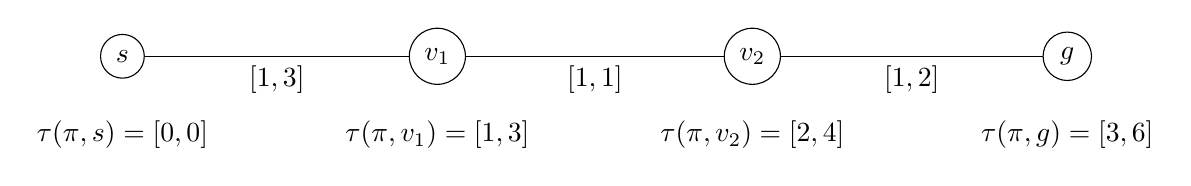
\begin{tikzpicture}[scale=1]
\tikzset{mapf-vertex/.style={circle, draw}}
\node[mapf-vertex] (s) at (0, 0) {$s$};
\node[mapf-vertex] (v1) at (4, 0) {$v_1$};
\node[mapf-vertex] (v2) at (8, 0) {$v_2$};
\node[mapf-vertex] (g) at (12, 0) {$g$};
\node at (0, -1) {$\tau(\pi, s) = [0, 0]$};
\node at (4, -1) {$\tau(\pi, v_1) = [1,3]$};
\node at (8, -1) {$\tau(\pi, v_2) = [2,4]$};
\node at (12, -1) {$\tau(\pi, g) = [3,6]$};

\draw (s) -- (v1) node [below,midway, fill=white] {$[1, 3]$};
\draw (v1) -- (v2) node [below,midway, fill=white] {$[1, 1]$};
\draw (v2) -- (g) node [below,midway, fill=white] {$[1, 2]$};
\end{tikzpicture}

\caption
{An example of the potential presence of the agent when moving from $s$ to $g$.}
%In this graph, an agent is traversing from initial vertex $s$ to goal vertex $g$. %The potential presence in each vertex is shown. Its potential presence at each vertex is defined by the equation in Definition 1.(1) no ref???(2) def 1 only comes later. I hate forward pointers in papers and try to avoid them}
\label{fig:potential-presence-ex}
\end{figure}
%
\begin{example}
(Figure~\ref{fig:potential-presence-ex}) Consider a single-agent plan $\pi$ in which the agent moves from its initial vertex $s$ to its goal vertex $g$ through vertices $v_1$ and $v_2$ without waiting. 
The time interval depicted above each edge is the range of possible edge durations. 
The \emph{potential presences} induced by $\vertexpath$ at vertices $s$, $v_1$, $v_2$, and $g$ are $\{[0, 0]\}$, $\{[1,3]\}$, $\{[2,4]\}$, and $\{[3,6]\}$, respectively. 
% Afterwards, at $v_1$ it is $[1,3]$ since it traversed only the edge $(s, v_1)$. At $v_2$ we compute the union of the minimum and maximum duration for the edge previously traversed and $(v_1, v_2)$ resulting in a potential presence of $[1+1, 3+1] = [2, 4]$. Similarly, the potential presence at goal vertex $g$ is $[3, 6]$.
\end{example}


% If an agent starts by moving to a vertex $v$, then its potential presence in $v$ is given by the minimum and maximum duration of the traversed edge. [[Roni: this is incorrect. What if the agent returns to that vertex later. This whole text is redunadant and not correct enough. Maybe have some of it later to explain the definition]
% If the agent then moves to a vertex $u$ then its potential presence in $u$ is the time interval between the sum of the minimum durations and the sum of the maximum durations of the traversed edges.
% If the agent continues traversing its single-agent plan and is currently at vertex $p$, then its potential presence there is the union over the intervals corresponding to each visit. 


% Computing the potential presence induced by a single-agent plan $\vertexpath$ 
% \begin{definition}

Computing the potential presence can be done as follows. 
Let $\vertexpath = \big((v_0,v_1) \dots (v_{n-1},v_n)\big)$ be a single-agent plan for some agent. 
For every $v_i\neq v_0$, the \emph{potential presence} induced by $\vertexpath$ is given by
%\dor{We defined a path as $v_0,v_1,..$.}
\begin{equation}
  \potential(\vertexpath, v) = \bigcup_{\!\!\!\!\!\!\!\!\substack{0 \leq i \leq n\\[0.2em] v_i = v}}\!\left[\sum_{0 \leq j < i\!\!\!\!\!} \timel(v_j, v_{j+1}), \sum_{\mathclap{0 \leq j < i}} \timeu(v_j, v_{j+1})\right]
\end{equation}
The potential presence induced by $\vertexpath$ on edge $(u, v)$ is given by
\begin{equation}
  \potential(\vertexpath, u, v) \!= \!\!\bigcup_{\!\!\!\!\!\!\!\!\substack{0 \leq i < n\\[0.2em] v_i = u\\[0.2em] v_{i+1} = v}}\!\!\!\left[\sum_{0 \leq j < i\!\!\!\!\!} \timel(v_j, v_{j+1}), \sum_{\mathclap{0 \leq j \leq i}} \timeu(v_j, v_{j+1})\right]\!\!
\end{equation}
In both of these formulas, when $i=0$ there are no values of $j$ that satisfy $0\leq j<i$. In this case, we consider the empty sum to be zero. 


\subsection{Potential Conflicts}
We are now equipped to define the different types of potential conflict that can occur in the MAPF-TU problem.
Two distinct single-agent plans have a \emph{potential vertex conflict} at some vertex $v \in \vertices$ if their potential presences in $v$ intersect. 
They have a \emph{potential edge conflict} at a pair of vertices $(u, v)$ if their potential presences intersect when traversing the edge in the same direction.  
They have a \emph{potential swapping conflict} at a pair of vertices $(u, v)$ if their potential presences intersect when traversing the edge in opposite directions. 
A solution $(\pi_1,\ldots,\pi_k)$ is \emph{safe} if it does not contain any potential conflict of these three types.  
That is, a solution is safe iff it satisfies the following
\begin{align}
\begin{split}
  \bigcup_{1 \leq i < j \leq k} \Big[&\bigcup_{v\in\vertices} \potential(\vertexpath_i, v) \cap \potential(\vertexpath_j, v)\\
  \cup&\bigcup_{u, v\in\vertices} \potential(\vertexpath_i, u, v) \cap \potential(\vertexpath_j, u, v)\\
  \cup&\bigcup_{u, v\in\vertices} \potential(\vertexpath_i, u, v) \cap \potential(\vertexpath_j, v, u)\Big] = \emptyset
\end{split}
\end{align}


% \begin{figure}[ht]
% \centering
% 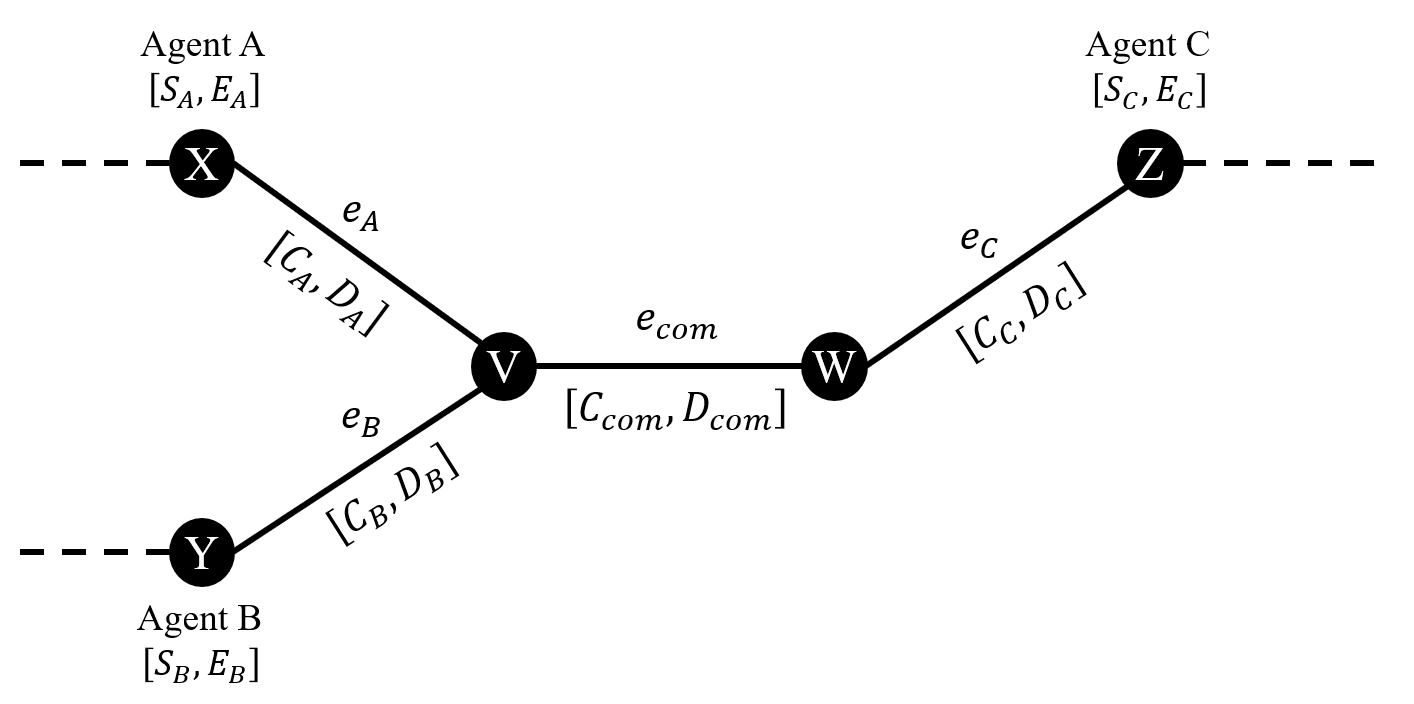
\includegraphics[width=7.5cm,height=4cm]{tu-graph.png}
% \caption{
% This MAPF-TU problem consists of three agents $A$, $B$, and $C$.
% %Captures three agents A, B, and C for the motivated MAPF problem. 
% The description of our complete approach is based on this diagram.}
% \label{fig:1}
% \end{figure}

%\shashank{Is it okay to remove this example? or maybe we should show all three type of conflicts. Currently, it just shows vertex conflict. Also, we use $a_i$ to represent an agent, not A.}\roni{Good catch}

% \subsection{How about this?: figure and example}

% \begin{figure}[ht]
% \centering
% \begin{tikzpicture}[scale=0.75]
% \tikzset{mapf-vertex/.style={circle, draw}}
% %%
% \node (x1) at (-0.5, 2) {};
% \node[mapf-vertex][label={$[l_{a_1}$,$u_{a_1}]$}] (x) at (1, 2) {$x$};
% \node (y1) at (-0.5, -2) {};
% \node[mapf-vertex] [label={ $[l_{a_2}$,$u_{a_2}]$}] (y)  at (1, -2) {$y$};
% \node[mapf-vertex] (v)  at (5, 0) {$v$};
% \node[mapf-vertex] (w) at (9, 0) {$w$};
% \node[mapf-vertex] [label={ $[l_{a_3}$,$u_{a_3}]$}] (z)  at (12.5, 2) {$z$};
% \node (z1) at (14, 2) {};
% %\node[mapf-vertex] (t1) at (2, -1) {$t_1$};
% %\node[mapf-vertex] (t2) at (2, -2) {$t_2$};
% %node at (7.5, -1.4) {$\sourcetargets = \tuple{(s_1, t_1), (s_2, t_2)}$};
% %%
% \draw (x1) -- (x) node [below, midway, fill=white] {};
% \draw (x) -- (v) node [below, midway, fill=white] { $[l_{xv}, u_{xv}]$};
% \draw (y1) -- (Y) node [below, midway, fill=white] {};
% \draw (Y) -- (V) node [above, midway, fill=white] { $[l_{yv}, u_{yv}]$};
% \draw (V)  -- (W) node [above, midway, fill=white] { $[l_{vw}, u_{vw}]$};
% \draw (z1) -- (Z) node [below, midway, fill=white] {};
% \draw (W) -- (Z) node [below, midway, fill=white] {$[l_{zw}, u_{zw}]$};
% \end{tikzpicture}

% \caption{A subgraph of a \mapftu instance that consists of vertices and edges that will be visited (or traversed) by agents $a_1$, $a_2$, and $a_3$ following their single-agent plans. For each agent $a_i$, its potential presence at a vertex is shown by $[l_{a_i}, u_{a_i}]$ along with the traversal times of the edges. On the way to their individual goals, $a_1$ is moving towards $z$ from $x$ ($x\rightarrow v \rightarrow w \rightarrow z$), $a_2$ is moving towards $z$ from $y$, and $a_3$ is moving towards $x$ from $z$.}
% \label{fig:naive-range-constraints1}
% \end{figure}


% \begin{example}
% (Figure~\ref{fig:naive-range-constraints1}) Agents currently follow single-agent plans $\pi_{a_1}$, $\pi_{a_2}$, and $\pi_{a_3}$, respectively. 
% %The potential presence of $a_1$ at $x$ induced by $\pi_{a_1}$ is $\tau(\pi_{a_1},x)$, i.e., $[S_A,E_A]$. Similarly, $\tau(\pi_B,Y)$ and $\tau(\pi_C,Z)$ are $[S_B,E_B]$ and $[S_C,E_C]$, respectively.
% %Based on the current execution, if the next action for $A$ is to traverse $e_A$ and for $B$ is to traverse $e_B$, their potential presence at $V$ is $[S_A+C_A,E_A+D_A]$ and $[S_B+C_B,E_B+D_B]$, respectively.
% Agents $a_1$ and $a_2$ following their plans occupy vertex $v$ in $[l_{a_1}+l_{xv}, u_{a_1}+u_{xv}]$ and $[l_{a_2}+l_{yv}, u_{a_2}+u_{yv}]$, respectively. The agents would have a {potential vertex conflict} if these two time intervals are not disjoint. 
% Suppose that $l_{a_1}=l_{a_2}=u_{a_1}=u_{a_2}=0$, $l_{xv}=l_{yv}=1$, $u_{xv}=2$, and $u_{yv}=3$, then the overall solution is not safe since $\pi_{a_1}$ and $\pi_{a_2}$ have a potential vertex conflict at $v$. 
% Similarly, $a_1$ and $a_2$ can have a {potential edge conflict}, and $a_1$ and $a_3$ can have a {potential swapping conflict}, while they are traversing edge $vw$ and their potential presences at $vw$ intersect.
% \label{example:not-safe}
% \end{example} 


% \shashank{end}

\subsection{Solution Cost}
In classical MAPF, it is common to define the cost of a solution as the sum-of-costs (SOC) of its constituent single-agent plans. 
However, in \mapftu the cost of a single-agent plan is ill-defined: 
the duration required to execute a single-agent plan is not known a-priori due to the uncertainty over edge duration. 
Therefore, we consider two alternative cost functions: \emph{optimistic} and \emph{pessimistic}. 
The \emph{optimistic} cost of a single-agent plan is the sum of 
lower bound ($\timel$) durations of all its constituent actions. 
This represents the earliest time in which the agent can reach its goal. 
The \emph{pessimistic} cost of a single-agent plan is the sum of 
upper bound ($\timeu$) durations of all its constituent actions. 
This represents the latest time in which the agent will reach its goal. 


Correspondingly, we consider two cost functions for a \mapftu solution: optimistic SOC and pessimistic SOC, 
denoted \socopt and \socpes, respectively. 
Other solution cost functions can also be envisioned, e.g., reducing the average cost of a solution or minimizing the size of the solution cost interval. 

%However, unless stated otherwise we will assume the pessimistic SOC cost function hereinafter and denote it by $SOC$. 



\section{\boldmath${\mathrm{A^* + OD}}$ under Time Uncertainty (\odatu)}
\label{odatu}

The first algorithm we propose for finding a safe solution to a \mapftu instance, called \odatu, builds on the \oda algorithm~\shortcite{standley2010finding} for classical MAPF.  
For completeness, we first provide a brief background on \oda.  

\subsection{\oda}
As its name suggests, \oda consists of running the \astar{} algorithm and using a technique called the Operator Decomposition (OD) technique~\shortcite{standley2010finding}. 
Specifically, \oda runs the well-known \astar{} algorithm to search the
\emph{$k$-agent search space}. 
A state in this search space is a vector of $k$ vertices representing the current location of each agent. 
An action in this search space is a \emph{joint action} of all agents, i.e., a vector of $k$ actions, one for each agent, which are performed concurrently in a single time step. 
A joint action is not legal if performing it would create a conflict between the agents. 
The number of joint actions applicable in a given state is exponential in the number of agents. 


% How does OD work
OD is a technique for keeping the branching factor of this search-space manageable 
by constructing joint actions in an incremental manner. 
Concretely, the agents are arranged in some fixed order. 
Then, when expanding a state, OD selects a single agent according to this order and 
generates child states by only considering the actions of the selected agent that are \emph{legal}. 
An action of the $i^{th}$ agent is legal if it does not conflict with the $i-1$ previously selected actions. 
Since the agents are selected in a fixed order, a sequence of $k$ actions constitutes a joint action for all agents, 
and states generated by such a joint action are \emph{standard states} of the $k$-agent search space. 
All other states are called \emph{intermediate states}, which represent the locations of some agents at some time step
and the locations of the other agents at the next time step. 
Given an admissible heuristic, \oda is a sound, complete, and optimal algorithm for classical MAPF. 




\subsection{\odatu}
% The number of actions applicable in each state can be exponential in the number of agents. Operator Decomposition (OD) is a technique designed to keep the branching factor of this search space manageable\cite{standley2010finding}. When using OD, the agents apply their actions one by one in a fixed order.

%It builds on the \astar+OD algorithm and adapts it to solve MAPF-TU instances, as follows. 
\odatu runs \astar in a search space in which a state is a vector of $k$ tuples 
\[ \big(\tuple{a_1,v_1,T_1}, \cdots, \tuple{a_k, v_k, T_k}\big)\]  
where every tuple $\tuple{a_i, v_i, T_i}$ represents that the potential presence of agent $a_i$ at vertex $v_i$ is $T_i$. 
% Formally, a state is represented as:
% $\left\langle\tuple{a_1, v_1, T_1}, \ldots , 
% \tuple{a_k, v_k, T_k}\right\rangle$, 
% where $T_i=[T_{i}^{\min},T_{i}^{\max}]$ is the potential presence of agent $a_i$ in location $v_i$ according to its single-agent plan so far. \roni{This is problematic, since the potential presence is a set of time intervals, not a single time interval.} 
Like OD, when a state is expanded \odatu chooses a single agent and generates a child state for every \emph{legal action} that agent can perform. 
However, in \odatu the agents are not chosen in a round-robin manner and the definition of a legal action is more complex, as we explain below. 

\subsubsection{Choosing the Next Agent in \odatu}


%
\begin{figure}[ht]
\centering
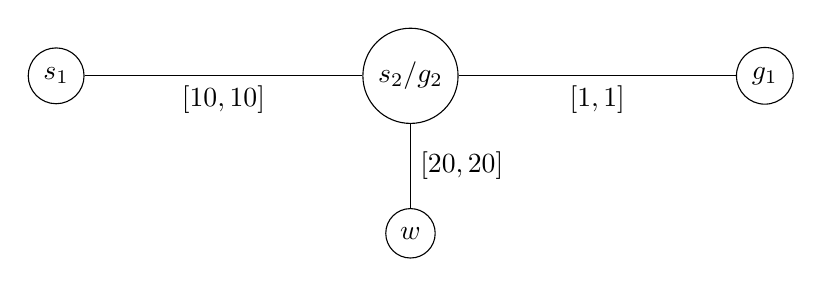
\begin{tikzpicture}[scale=1]
\tikzset{mapf-vertex/.style={circle, draw}}
\node[mapf-vertex] (s1) at (0.5, 0) {$s_1$};
%\node[mapf-vertex] (s2) at (0.5, -2) {$s_2$};
\node[mapf-vertex] (t2) at (5, 0) {$s_2/g_2$};
\node[mapf-vertex] (t1) at (9.5, 0) {$g_1$};
\node[mapf-vertex] (w) at (5, -2) {$w$};
%\node at (8.5, -1.7) {$\sourcetargets = \tuple{(s_1, g_1), (s_2, g_2)}$};
%
\draw (s1) -- (t2) node [below,midway, fill=white] {$[10, 10]$};
\draw (t1) -- (t2) node [below,midway, fill=white] {$[1, 1]$};
\draw (w) -- (t2) node [right,midway, fill=white] {$[20,20]$};
\end{tikzpicture}
%
\caption
{
This is an example where a trivial round-robin order of \odatu returns an illegal solution for a weighted graph, even without uncertainty.% The \emph{initial} and \emph{goal} locations for both agents are listed at bottom right.
}
\label{oda-fail}
\end{figure}


Choosing agents in a round-robin manner as done by \oda may lead to an unsafe solution for \mapftu. 
For example, consider the \mapftu instance depicted in Figure~\ref{oda-fail}.
%\dor{Figures 1,2, and 3 look different from each other. We should consider presenting a uniform representation.} 
Agent $a_2$ is at its goal location ($g_2$) which is also its initial location ($s_2$) and agent $a_1$'s goal is $g_1$ and its initial location is $s_1$. 
%\dor{"initial" and "goal" or "start" and "end"?} 
Suppose a round-robin order is followed, and $a_1$ is followed by $a_2$. The search begins, $a_1$ moves to $s_2$ and occupies it at $[10,10]$. 
Next, $a_2$ waits at its goal, since it is already at its goal location. Consequently, the resulting state would be 
$\big(\tuple{a_1, s_2, \{[10,10]\}}, \tuple{a_2, s_2, \{[1,1]\}}\big)$. 
Then, $a_1$ again moves to $g_1$ and $a_2$ waits at $g_2$, resulting in a goal state, 
$s_g = \big(\tuple{a_1, s_2, \{[11,11]\}}, \tuple{a_2, s_2, \{[2,2]\}}\big)$.  
%\dor{Did we assume that a wait action costs [1,1]?}
%\shashank{yes}
All moves taken up to this point are valid but the resulting solution is not safe, since $a_2$ cannot continue waiting there indefinitely. 


To avoid this problem, in every iteration of \odatu the agent with the potential presence having the minimal optimistic bound is selected.
%For reviewer 1
\footnote{This is similar to tracking the agent controller that complete its assigned task first in a multi-robot navigation setup, as done by Wagner et al.~\citeyear{wagner2016multirobot}.}
For example, in a \odatu state 
$\big(\tuple{a_1, v_1, \{[1,6]\}},\tuple{a_2, v_2, \{[2,4]\}}\big)$ we will choose to expand this state with agent $a_1$. 
If this approach is applied in the example above (Figure~\ref{oda-fail}), $a_1$ still moves first and $a_2$ performs the second action, but then $a_2$ continues waiting at $g_2$ until $[9,9]$. 
Then, waiting in $g_2$ will raise a conflict, which will eventually lead the search to find a safe solution.
% Reviewer
Note that the distinction between standard states and intermediate states is not relevant for \odatu\ as the same agent may move multiple times and the number of actions has no inherent value. 
A similar form of OD-style expansion was suggested by Walker~\citeyear{walker2018extended} in the E-ICTS algorithm. 


% Choosing to generate child states for the agent with the earliest potential presence is important, since the round-robin agent selection used by \oda may lead to an unsafe solution. 
% %as other design choices may result in returning an unsafe solution. [[roni: the example shows that round-robin is unsafe, not that every other design choice is unsafe]
% For example, consider Figure~\ref{oda-fail}.
% %\dor{Figures 1,2, and 3 look different from each other. We should consider presenting a uniform representation.} 
% Agent $a_2$ is at its goal location ($g_2$) which is also its initial location ($s_2$) and agent $a_1$'s goal is $g_1$ and its initial location is $s_1$. 
% %\dor{"initial" and "goal" or "start" and "end"?} 
% If a round-robin ordering is followed, say $a_1$ is followed by $a_2$. The search begins, $a_1$ moves to $s_2$ and occupies it at $[10,10]$. 
% Next, $a_2$ waits at its goal, since it is already at its goal location, consequently the resulting state would be $\tuple{\tuple{a_1, s_2, \{[10,10]\}}, \tuple{a_2, s_2, \{[1,1]\}}}$. 
% Then, $a_1$ again moves to $g_1$ and $a_2$ waits at $g_2$, resulting in a goal state, $s_g = \tuple{\tuple{a_1, s_2, \{[11,11]\}}, \tuple{a_2, s_2, \{[2,2]\}}}$.  
% %\dor{Did we assume that a wait action costs [1,1]?}
% %\shashank{yes}
% All moves taken up to this point are valid but the resulting solution is not safe, since $a_2$ cannot continue waiting there indefinitely. 
% If our approach is applied, $a_1$ still moves first and $a_2$ performs the second action, but then $a_2$ continues waiting at $g_2$ until $[9,9]$. 
% Then, waiting in $g_2$ will raise a conflict, which will eventually lead the search to find a safe solution.

%Note that \oda\ has a notion of \emph{intermediate nodes} and \emph{standard nodes}. \emph{Intermediate nodes} are nodes where not all agents have performed an action and a \emph{standard node} is one where all agents have performed exactly the same number of actions, \eg\ the start state where no agent has moved yet. These notions are irrelevant for \odatu\ as the same agent may move multiple times and the number of actions has no inherent value. \roni{I'm not sure if this doesn't confuse more than help}


\subsection{Identifying Legal Actions}

% there are two key differences. 
% First, instead of choosing agents in a fixed order, we choose in every iteration the agent with the potential presence containing the minimal optimistic bound is selected. 
% For example, in a \odatu state 
% $(\tuple{a_1, v_1, \{[1,6]\}},\tuple{a_2, v_2, \{[2,4]\}})$ we will choose to expand this state with agent $a_1$. 
% Second, to check if an action is legal for an agent in a state, it is not sufficient to check if it raises a potential conflict in the resulting state. 
% We also need to check if it raises a potential conflict with the other agents in any of the states that are resulting from appl

The second significant difference between \oda and \odatu is what constitutes a legal action for an agent. 
In \oda, it is sufficient to check that the chosen action of agent $a_i$ does not conflict with one of the $i-1$ agents that were already chosen for an action in this time step. 
In~\odatu, we must check if an action creates a conflict with any of the actions performed by the other agents in any of the predecessors of the current state. 
This is done by traversing up the parent and parent-of-parent of the current node until either we find a conflict or can guarantee that such a conflict does not exist. This can be guaranteed when reaching a predecessor state in which the maximum time of the potential presences of all other agents is lower than the minimum time of the potential presence of the current agent. 

% a move is determined to be valid or not, presented in Algorithm~\ref{algo.validateMove}. 






% Second, to check if an action is legal for an agent in a state, it is not sufficient to check if it raises a potential conflict in the resulting state. 
% We also need to check if it raises a potential conflict with the other agents in any of the states that are resulting from appl


% the definition of a \emph{legal action} of an agent in a state is more a legal action of an agent in \odatu is an action that does not create a potential conflict with the potential presences of the other agents in the resulting state as well as all the potential presences of the other agents in all parent states. 

% In~\odatu, for every optional action, we must check if it creates a conflict with one of the actions performed by the parents of the current state. 
% This is done by traversing up the parent and parent-to-parent of the current node (Line~14, Algorithm~\ref{algo.validateMove}) until either we find a conflict \emph{or} the max time of the potential presences of all other agents is lower than the minimal time of the current agent (Line~11). 



% % The intuition for choosing agents by their optimistic potential presence rather than iterating through agents in a fixed order, as in \oda, is that otherwise the \emph{times} of each agent's potential presence may vary wildly and detecting potential conflicts becomes computationally harder.
% % This is because we are searching for intersecting times. 
% % Letting the \emph{"earliest"} agent move first ensures that there is less variation in an agent's \emph{time} (potential presence).
% % \roni{MAJOR ISSUE: This is *very* hand wavy and not clear. I thought doing the fixed order is incorrect, no? this paragraph is not helping. Sufficient to show the example below}
% \roni{What about explaining the need to check parent states?}


% The pseudo-code to check the validity of a move is depicted in  Algorithm~\ref{algo.validateMove}.
% A child state is generated for every action the agent may perform from its current location which does not raise any conflict with the other potential presences and the potential presences in any of its parent states.
% Note that checking the potential presence of parent states is necessary to ensure that the current movement does not conflict with previously planned movements. 
% In~\odatu, for every optional action, we must check if it creates a conflict with one of the actions performed by the parents of the current state. 
% This is done by traversing up the parent and parent-to-parent of the current node (Line~14, Algorithm~\ref{algo.validateMove}) until either we find a conflict \emph{or} the max time of the potential presences of all other agents is lower than the minimal time of the current agent (Line~11). 
% %\dor{aThe last sentence is hard to follow.}

% \begin{algorithm}[h!]
%   \KwIn{agent $a_i$; 
%         action, $curr\_op$; 
%         state after $a_i$ performs $curr\_op$, $N$}
%   \KwOut{\emph{Valid} OR \emph{Invalid}}
%   \SetAlgoLined
%   \While{True}
%   {
%     \If{
%         $\exists a_j \neq a_i \text{ such that }$ \\ %\textcolor{red}{// verifies newly generated state}\\ 
%             ~$N[a_i].loc_i = N[a_j].loc_j$ \textbf{and}\\
%             ~$N[a_i].T_i \cap N[a_j].T_j \neq \emptyset$
%     }{\textbf{return} \emph{Invalid}}
%     %
%     $last\_op \leftarrow (parent(N)).leading\_op$; 
%     \textcolor{red}{~~//~~leading operator is the move that generated the parent node} \\ 
%     \If{
%         $last\_op.a_j \neq a_i$ \textbf{and} \\
%         ~$last\_op.T_j \cap curr\_op.T_i \neq \emptyset$ \textbf{and} \\
%         ~$last\_op.e = curr\_op.e$
%     }
%     { \textbf{return} \emph{Invalid} } 
%         \If{
%     $\forall a_j \text{ such that } a_j \neq a_i$ \textbf{ it holds that } $last\_op.T^j_{max} < curr\_op.T^i_{min}$
%     %        $a_i \neq a_j$ \textbf{and}  $last\_op.T^j_{max} < curr\_op.T^i_{min}$
%         }
%         {
%             \textbf{return}  \textit{Valid} 
%         }
%         \Else{
%             $N \leftarrow parent(N)$
%         }
%     %}
%   }   
%   \caption{\emph{ValidMove()}: confirms whether $a_i$'s current \emph{move} is valid.}
%   \label{algo.validateMove}
% \end{algorithm}

\subsection{Optimality}

% g and h values
\odatu\ runs \astar\ over the search space defined above, 
computing for every generated state $N$ its $g$ and $h$ values, and expanding in every iteration a state with the minimal $g+h$ value in the open list. 
The definition of $g$ and $h$ depends on the objective function we want to optimize, \socopt or \socpes. 
If we aim to optimize \socopt, then the $g$ value is the sum over the \emph{lower} time-bound in each potential presence. If we aim to optimize \socpes, then the $g$ value is the sum over the \emph{upper} time bound in each potential presence. 


Let $C^*$ be the optimal solution cost for the chosen objective. 
A heuristic for a state $N$ is admissible if it is a lower bound on $C^*-g(N)$.  
The admissible heuristic we used is based on the Sum of Individual Costs (SIC) heuristic, which is commonly used in classical MAPF. SIC is the sum of costs of the agents' lowest-cost single-agent plans when ignoring all other agents. 
For \mapftu, the costs in the SIC computation depend on the objective function. 
When computing SIC for the \socopt objective, then it is the sum of the \emph{optimistic cost} of the single-agent plans that have the lowest \emph{optimistic cost}. 
When computing SIC for the \socpes objective, then it is the sum of the \emph{pessimistic cost} of the single-agent plans that have the lowest \emph{pessimistic costs}. 
%
%The last component of \odatu is a conflict detection mechanism. \odatu only generates states created by a move that does not cause a conflict with all the actions in the agents' path so far. 
%

%\subsection{Theoretical Properties}

%\abda{we haven't formally defined what it means for an algorithm to be sound.}
\begin{theorem}
\odatu is guaranteed to return an optimal safe solution if such a solution exists, such that it is sound, complete, and optimal. 
\label{the:aod}
\end{theorem}
\begin{proofo}
Soundness follows directly from the fact that a state is generated only if it does not create any potential conflict with the previously chosen actions according to their potential presences. 
\odatu\ is a best-first search, maintaining all non-conflicting nodes it generates in the open list. Thus completeness follows.
\odatu halts when a goal state $N_g$ is expanded. 
Since we expand in every iteration the state with the minimal $g+h$ and 
the $h$ of every goal state is zero, 
then $g(N_g)\leq g(N)+h(N)$ for every state $N$ in the open list. 
Since $h$ is admissible, 
we have that $g(N_g)$ is optimal, as required. %\dor{Maybe we should add something on the behavior of the g-value (or f-value) during the search -- that it cannot decrease.}
\end{proofo}
%\shashank{We need to connect the last example and the pseudo code well.}
%\begin{proof}
%\end{proof}
%\begin{theorem}
%The \odatu algorithm returns an optimal solution.
%\end{theorem}
%\begin{proof}
%\end{proof}

%\roni{Please read the subsection above carefully, I edited it.}\tomer{looks fine}

\section{CBS under Time Uncertainty (\cbstu)}
\label{cbstu}

The second algorithm we propose for \mapftu is called \cbstu. 
\cbstu is based on the Conflict-Based Search (CBS) algorithm~\shortcite{sharon2015conflict}. 
For completeness, we provide a brief description of CBS. 


\subsection{Conflict Based Search (CBS)}


CBS~\shortcite{sharon2015conflict} is a complete and optimal MAPF solver, designed for classical MAPF.
CBS finds a solution by iteratively planning for each agent separately, detecting \emph{conflicts} between these single-agent plans, and resolving them by replanning for the individual agents subject to specific \emph{constraints}. 
A CBS conflict is defined by a tuple $\tuple{a_i, a_j, x, t}$, representing that there is a conflict between agents $a_i$ and $a_j$ at vertex/edge $x$ at time $t$. 
A CBS constraint is defined by a tuple $\tuple{a_i,x,t}$, representing that agent $a_i$ cannot occupy $x$ at time step $t$, where $x$ is either a vertex or an edge. 
To choose which constraints to add to which agent, CBS maintains a Constraint Tree (CT). 
The CT is a binary tree, in which each node $N$ represents a solution ($N.\sol$) and a set of constraints ($N.\const$). 
If $N.\sol$ is a valid solution then $N$ is referred to as a goal CT node.
Therefore, if $N$ is not a goal CT node then $N.\sol$ has a conflict.
Expanding a non-goal CT node $N$ means choosing a conflict $\tuple{a_i,a_j,x,t}$, and generating two child CT nodes $N_i$ and $N_j$. 
The constraints of $N_i$ and $N_j$ are all the constraints of $N$, as well as the constraints $\tuple{a_i,x,t}$ and $\tuple{a_j,x,t}$, respectively. 
Then, a search algorithm such as \astar is used to generate a single-agent plan for agent $a_i$ that satisfies the constraints in $N_i$, and to generate a single-agent plan for agent $a_j$ that satisfies the constraints in $N_j$. 
The search algorithm used for finding these single-agent plans is referred to as the \emph{CBS low-level search}. 
These single-agent plans are used in their respective CT nodes instead of the single-agent plans for the constrained agent in $N$. 


CBS searches the CT in a best-first manner according to the cost of the solution in each CT node.
The search halts when a goal CT node is chosen for expansion. 
This best-first search is referred to as the \emph{CBS high-level search}.
Many improvements have been suggested to the basic CBS algorithm over the years~\shortcite{felner2018adding,lazy-cbs,branch-cut_price,li2019symmetry}.
% \shashank{[[Added below about ICBS, new text until section 3]]}


\subsection{From CBS to \cbstu}
\cbstu is an adaptation of CBS for solving \mapftu instances. 
It requires changing how conflicts are defined, how they are resolved, and how the low-level search operates. 
We describe these changes in detail next. 

%The previous section explained one way to find out whether two paths are conflicting. Following the example scenario in Figure~\ref{fig:1}, we now explain how such conflicts can be resolved. Our approach of resolving such conflicts, is an adaptation of the approach used in CBS algorithm. 

\subsubsection{Conflicts over Potential Presences}
There is a \cbstu conflict in a solution $\Pi$ iff 
there is a potential conflict in $\Pi$.  
A \cbstu constraint is defined by a tuple $\tuple{a_i,a_j,x,T}$, 
where $a_i$ and $a_j$ are the conflicting agents, $x$ is the vertex or edge in which the potential conflict exists, 
and $T$ is the intersection between the potential presences of $a_i$ and $a_j$ on $x$. 
That is, if $\pi_i$ and $\pi_j$ are the single-agent plans for $a_j$ and $a_j$ then 
$T=\tau(\pi_i, x)\cap \tau(\pi_j, x)$. 
Recall that in \mapftu there may be edge, vertex, and swapping potential conflicts. 
Thus, there are respective \cbstu conflicts that may occur.  
%\roni{There was a bunch of detailed text here about the types of conflicts. This repeats what is already in the problem definition part. If anyone sees a reason to uncomment the additional text on this, let me know}.\shashank{yes, repeated text.}
% In CBS, a conflict is defined by the tuple $\tuple{a_i,a_j,x,t}$, that represents the agents $a_i$ and $a_j$ occupy $x$ --- which can be a vertex or an edge --- at time $t$.
% In \mapftu, 

% \emph{potential conflicts} are defined over potential presences of the agents. Specifically, we consider the following types of potential conflicts.

% \paragraph{Potential vertex conflict.} 
% A vertex conflict is defined by the tuple $\tuple{a_i,a_j,v,T}$ 
% and represents that the potential presences of agents $a_i$ and $a_j$ at vertex $v$, induced by the 

% have a potential vertex conflict at vertex $v$ and the intersection of their potential presences is the range $T = \tau(\pi_i,v) \cap \tau(\pi_j,v) \neq \emptyset$. 



% %That is, there is a conflict between paths $\pi_i$ and $\pi_j$ at vertex $v$ iff their potential presences intersect.
% Thus, a vertex conflict for the CBSTU algorithm is defined by the tuple $\tuple{a_i,a_j,v,T}$
% and it represents that agents $a_i$ and $a_j$ have a potential vertex conflict at vertex $v$ and the intersection of their potential presences is the range $T = \tau(\pi_i,v) \cap \tau(\pi_j,v) \neq \emptyset$. 
% %An edge conflict in CBSTU is defined in a similar way.
% %
% %
% %However, unlike the CBS approach, we have two types of conflict that are related to edges. 

% Agents can not only collide when they traverse an edge in the opposite directions (swapping conflict), but also when they traverse it in the same direction (edge conflict). %\dor{Isn't it an edge conflict and not a swapping conflict? From the background: "Following the terminology of Stern et. al. (2019), we
% %only consider vertex, edge, and swapping con
% %icts."}\roni{TODO: Move this discussion to the problem definition section. There, talk about how in classical MAPF vertex conflict subsumes edge conflict but here it does not, as we have these conflicts below}
% Next, we explain the potential edge and swapping conflicts.
% %

% \paragraph{Potential Edge Conflict:} 
% this type of an edge conflict is represented as: 
% $\mathit{(A,C,e_{com}, \tau(\pi_A,e_{com}),\tau(\pi_C,e_{com}), T)}$, which refers as agents $A$ and $C$ could potentially occupy edge $e_{com}$ simultaneously, at $T$, while traversing the edge $e_{com}$ in the same direction, such that $T= \tau(\pi_A,e_{com}) \cap \tau(\pi_C,e_{com}) \neq \emptyset$.
% We note that we can have this type conflict only when $e_{com}$, $D_{com} > C_{com} \geq 1$. 
% %\dor{In both conflicts here I didn't understand if the agents are A and B, or A and C. Also, this is no based on Figure 1.}
% %
% %Based on how a vertex conflict is resolved in our MAPF framework, to \textit{resolve} this type of an edge conflict, we must restrict one of the agents to occupy $e_{com}$ at $[t_1,t_2] = \tau(\pi_A,e_{com}) \cap \tau(\pi_B,e_{com})$. 
% %Simply restricting agents for whole $[t_1,t_2]$ would make the algorithm incomplete, e.g., a situation exactly like the one we provide with for the vertex conflict case.
% %%
% %Therefore one way to resolve this is by restricting A with a constraint: $occupy(A,e_{com},t)$ where $t \in [t_1,t_2]$. The constraint specifies that A is not allowed to occupy edge $e_{com}$ at $t$. 
% %Similarly, B can be restricted using the constraint: $occupy(B,e_{com},t)$ s.t. $t \in [t_1,t_2]$. To guarantee solution optimality we examine both these possibilities. 

% \paragraph{Potential Swapping Conflict} 
% %The other type of edge conflict is a bit more subtle. It arises when two agents traverse an edge in opposite directions simultaneously.
% %
% %A bit complex case compared to the first one as some subtle issues might arise, is defined as \emph{head-on} collision -- when two agents traversing an edge in opposite directions simultaneously.
% %
% %A simple case is, which is also easy to detect, when two agents traverse an edge in opposite directions and they possibly occupy the edge together at $[t_1,t_2]$, computed in a similar manner. 
% %For example, in Figure~\ref{fig:1}, agent A reaches V at $[S_A+C_A,E_A+D_A]$ and another agent C reaches W at $[S_C+C_C,E_C+D_C]$, and they traverse in the opposite directions. Agent A could occupy $e_{com}$ at $T_A = [S_A+C_A+1,E_A+D_A+D_{com}-1]$ while agent C could occupy it at $T_C = [S_C+C_C+1,E_C+D_C+D_{com}-1]$. 
% %There is an edge conflict if $[t_1,t_2] = T_A \cap T_C \neq \emptyset$. 
% %Perhaps such conflicts are also possible when $T_A \cap T_C = \emptyset$ under certain conditions, which is based on head-on conflict in the standard CBS algorithm. 
% %For example, when A reaches V at $[3,3]$ and C reaches W at $[3,3]$, and $[C_{com},D_{com}] = [1,1]$. 
% %In Figure~\ref{fig:1}, this case is possible when $S_A+C_A = E_A+D_A$, $S_C+C_C = E_C+D_C$ and $C_{com}=D_{com}=1$. Assuming that $D_{com} \geq C_{com} \geq 1$, there is a proper edge conflict where agents can occupy the edge for some time interval. 
% % Based on Figure~1, 
% % this type of an edge conflict is represented as:  
% % $(A,C,e_{com},\tau(\pi_A,e_{com}),\tau(\pi_C,e_{com}), [C_{com},D_{com}])$,
% % reads as agents A and C could potentially occupy edge $e_{com}$ simultaneously while traversing this edge in the opposite directions, such that $\tau(\pi_A,e_{com}) \cap \tau(\pi_B,e_{com}) \neq \emptyset$.

% Based on Figure~1, 
% this type of an edge conflict is represented as: 
% $\mathit{(A,B,e_{com}, \tau(\pi_A,e_{com}),\tau(\pi_B,e_{com}), T)}$, that implies that agents $A$ and $C$ could potentially occupy edge $e_{com}$ simultaneously, at $T$, while traversing the edge $e_{com}$ in the opposite directions, such that $T= \tau(\pi_A,e_{com}) \cap \tau(\pi_B,e_{com}) \neq \emptyset$.
% %
% %However marking the direction of movement for an agent is not important as the time interval in the representation suffices. 
% %
% %We resolve this conflict in the same way we resolve a run-over conflict. It generates two new children with two new constraints $occupy(A,e_{com},t)$ and $occupy(C,e_{com},t)$ respectively for agents A and C. They inherit all their parent's constraints. 
% %
% % To resolve conflicts of this kind, we restrict, at least, one of A and C to start its current move at \emph{time} that possibly enables the agent to occupy $e_{com}$ at an instance $t \in [t_1,t_2]$. 
% % Following our previous description, first we restrict A using the constraint {$(\neg move(A,e_{com},t-1) \wedge \neg move(A,e_{com},t-2) \wedge ... \wedge \neg move(A,e_{com},t-(D_{com}-1))$. Similarly, in the second approach we restrict B using the constraint {$(\neg move(B,e_{com},t-1) \wedge \neg move(B,e_{com},t-2) \wedge ... \wedge \neg move(B,e_{com},t-(D_{com}-1))$, for all $t \in [t_1,t_2]$. 
% %To guarantee optimality both these possibilities are examined. 
% %This captures all possible scenarios that could ever cause a head-on collision.
% %
% Although we can capture all possible potential conflicts when they are likely to  occupy an edge simultaneously, but this approach cannot capture a case when $\tau(\pi_A,e_{com}) \cap \tau(\pi_C,e_{com}) = \emptyset$, i.e., when two agents try to swap their positions via traversing edge $e_{com}$, and $[C_{com}, D_{com}] = [1,1]$. In this case, $T=\phi$, and this specific type of conflict is dealt the same way the basic CBS approach tackles it.  

%
% To resolve this special type of edge conflict, again two children are generated and are explored to guarantee solution optimality.
% Left child restricts agent A by $occupy(A,e_{com},(S_A+C_A + C_{com}/2))$, and in the right C is restricted by $occupy(C,e_{com},(S_C+C_C + C_{com}/2))$. Note that, $(S_A+C_A + C_{com}/2) = (S_C+C_C + C_{com}/2)$. The children directly inherit all the parent's constraints. 
% 
% First restrict A using $move(A,e_{com},S_A+C_A)$, and in the other solution restrict C using $move(C,e_{com},S_C+C_C)$.   
% We are not over constrained with this approach of resolving a head-on conflict and hence do not miss out on any possible solution, consequently, preserving the completeness.

% The above discussed approaches to resolve various kind of conflicts, guarantee that we do not lose the completeness. 
% We always return a valid solution if there exists one. 
% However, we do suspect that there would be some optimistic way to choose $t \in [t_1,t_2] = \tau(\pi_A,e_{com}) \cap \tau(\pi_C,e_{com})$, instead of an arbitrary, or rather two or more contiguous $t$'s after some preprocessing of the given problem graph. 
% This probably would not improve the worst case theoretical guarantees discussed later in the paper, but could improve things practically. 

%\dor{I decided not to move the potential conflicts to the background. In the background we do describe the potential conflicts and here we only give examples to them and talk about their relation to CBSTU. I did change the text a bit.}OK

\subsubsection{Resolving a Conflict}

One may be tempted to resolve a \cbstu conflict $\tuple{a_i,a_j,v,T}$ by imposing \emph{range constraints}, which are constraints that prevent an agent from occupying any time step in time range $T$.
Range constraints have been shown to be useful in CBS~\shortcite{atzmon2020robust,li2019symmetry}. 
Unfortunately, using these kind of range constraints in our context would lead to a suboptimal or even incomplete algorithm, as shown in the following example.


% \begin{figure}[ht]
% \centering
% \begin{tikzpicture}[scale=0.75]
% \tikzset{mapf-vertex/.style={circle, draw}}
% \node[mapf-vertex] (s1) at (0.5, 0) {$s_1$};
% \node[mapf-vertex] (a)  at (2.5, 2) {$A$};
% \node[mapf-vertex] (t2)  at (5, 0) {$g_2$};
% \node[mapf-vertex] (s2) at (9.5, 0) {$s_2$};
% \node[mapf-vertex] (b)  at (7.5, 2) {$B$};
% \node[mapf-vertex] (t1) at (2, -1) {$g_1$};
% %\node[mapf-vertex] (t2) at (2, -2) {$v_2$};
% % \node at (7.5, -1.4) {$\sourcetargets = \tuple{(s_1, g_1), (s_2, g_2)}$};

% \draw (s1) -- (a) node [above left,midway, fill=white] {$[1, 1]$};
% \draw (s1) -- (t2) node [above,midway, fill=white] {$[2, 4]$};
% \draw (a)  -- (t2) node [above right,near start, fill=white] {$[2, 2]$};
% \draw (s2) -- (b) node [above right,midway, fill=white] {$[2, 2]$};
% \draw (s2) -- (t2) node [above,midway, fill=white] {$[1, 5]$};
% \draw (b)  -- (t2) node [above left,near start, fill=white] {$[2, 2]$};
% \draw (t2) -- (t1) node [below right,near end, fill=white] {$[1, 1]$};
% %\draw (c) -- (t2) node [below right,near end, fill=white] {$[1, 1]$};
% \end{tikzpicture}

% \caption{A \mapftu instance showing that using naive range constraints in \cbstu leads to suboptimal solutions.
% %The initial and goal vertices of the two agents are indicated in the bottom right.
% }
% \label{fig:no-range-conflicts}
% \end{figure}
% \begin{example}
% Consider the \mapftu instance depicted in Figure~\ref{fig:no-range-conflicts}, 
% and assume the objective is to minimize optimistic SOC. 
% The initial solution $\Big\{\big((s_1, g_2), (g_2, g_1)\big),\big((s_2, g_2)\big)\Big\}$ has a vertex conflict $\tuple{a_1,a_2,g_2,[2,4]}$.
% %
% However, imposing the constraints that agent $a_1$ or agent $a_2$ cannot visit $g_2$ at any time step in $[2,4]$ rules outs the optimal solution 
% \[ \Big\{\big((s_1, A), (A, g_2), (g_2, g_1)\big),\big((s_2, B), (B, g_2)\big)\Big\} \]
% %$(s_1Ag_2g_1,s_2Bg_2)$. %\dor{We defined a path as $v_1,v_2,...$ (with commas).}
% %consider that $[S_A,E_A] = [0,0]$ and $[S_B,E_B] = [0,0]$.
% %The time ranges for the edges XV and YV are $[C_A,D_A] = [5,11] \text{ and } [C_B,D_B] = [7,18]$, respectively.
% %Suppose that there are two more edges XV and YV having the time ranges of $[8,9] \text{ and } [9,10]$, respectively. 
% %If the search optimizes on lower-time bound, the algorithm would place a strong constraint, $[t_1,t_2] = [7,11]$, on vertex $V$ in the first go.
% %Therefore at least one agent is not allowed to occupy $V$ in $[7,11]$ in all possible solutions.
% %
% %This strong constraint guarantees that the approach would miss the only possible solution. 
% %The agents are not allowed to move via other two edges XV and YV.
% \end{example}
% \abda{See Figure~\ref{fig:no-range-conflicts-correct} for an attempt at a correct counter-example. If we like it, then let's not forget to adapt the Example text below (adjust the range from [2, 4] to [1, 4].}

\begin{figure}[ht]
\centering
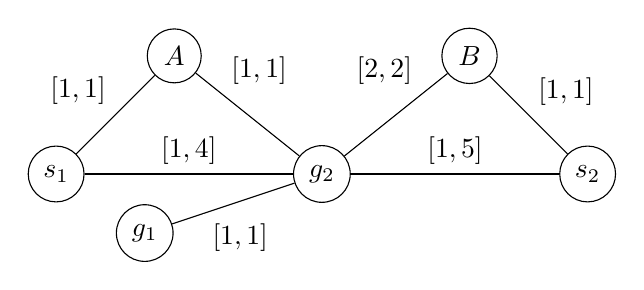
\begin{tikzpicture}[scale=0.75]
\tikzset{mapf-vertex/.style={circle, draw}}
\node[mapf-vertex] (s1) at (0.5, 0) {$s_1$};
\node[mapf-vertex] (a)  at (2.5, 2) {$A$};
\node[mapf-vertex] (t2)  at (5, 0) {$g_2$};
\node[mapf-vertex] (s2) at (9.5, 0) {$s_2$};
\node[mapf-vertex] (b)  at (7.5, 2) {$B$};
\node[mapf-vertex] (t1) at (2, -1) {$g_1$};
%\node[mapf-vertex] (t2) at (2, -2) {$v_2$};
% \node at (7.5, -1.4) {$\sourcetargets = \tuple{(s_1, g_1), (s_2, g_2)}$};

\draw (s1) -- (a) node [above left,midway, fill=white] {$[1, 1]$};
\draw (s1) -- (t2) node [above,midway, fill=white] {$[1, 4]$};
\draw (a)  -- (t2) node [above right,near start, fill=white] {$[1, 1]$};
\draw (s2) -- (b) node [above right,midway, fill=white] {$[1, 1]$};
\draw (s2) -- (t2) node [above,midway, fill=white] {$[1, 5]$};
\draw (b)  -- (t2) node [above left,near start, fill=white] {$[2, 2]$};
\draw (t2) -- (t1) node [below right,near end, fill=white] {$[1, 1]$};
%\draw (c) -- (t2) node [below right,near end, fill=white] {$[1, 1]$};
\end{tikzpicture}
\caption{A \mapftu instance showing that using naive range constraints in \cbstu leads to suboptimal solutions.
%The initial and goal vertices of the two agents are indicated in the bottom right.
}
\label{fig:no-range-conflicts}
\end{figure}
\begin{example}
Consider the \mapftu instance depicted in Figure~\ref{fig:no-range-conflicts}, 
and assume the objective is to minimize optimistic SOC. 
The initial solution $\Big\{\big((s_1, g_2), (g_2, g_1)\big),\big((s_2, g_2)\big)\Big\}$ has a vertex conflict $\tuple{a_1,a_2,g_2,[1,4]}$.
However, imposing the constraints that agent $a_1$ or agent $a_2$ cannot visit $g_2$ at any time step in $[1,4]$ rules outs all optimal solutions. Specifically, in all optimal solutions agent $a_1$ has the single-agent plan $\big((s_1,A), (A,g_2), (g_2, g_1)\big)$ and agent $a_2$ has a single-agent plan in which $a_2$ arrives to $g_2$ at time step 4 (either by waiting at $s_2$ for 3 time steps of by moving through $B$).
\end{example}
In fact, we can even show that sometimes even restricting an agent for two consecutive time steps
%\dor{time steps?}, 
$t$ and $t+1$, such that $t$ and $t+1$ belong to $T$, makes the approach suboptimal or even incomplete.
%
Thus, we resolve a vertex conflict $\tuple{a_i,a_j,v, T}$ by choosing a single time step $t \in T$, and creating two Constraint Tree (CT) nodes $N_i$ and $N_j$ with the added constraints $\tuple{a_i, v ,t}$ and $\tuple{a_j, v,t}$ respectively. 
Any time step $t$ in $T$ is a valid choice. 
The same strategy is used for resolving edge and swapping conflicts.\footnote{See Appendix~\ref{appendix:edge-constraint} for an example similar to Figure~\ref{fig:no-range-conflicts}, demonstrating why range constraints cannot be trivially used to resolve a swapping conflicts.}
%, following its representation.
%Except for the case when $[C_{com},D_{com}]=[1,1]$. We... \shashank{Tomer, how do we resolve it when $C_{com},D_{com}$ is [1,1]?}
The above approach preserves optimality and completeness, since we know that in any valid solution at most one of the conflicting agents can occupy the conflict location at a given instant. 




One may consider imposing range constraints over edges to indirectly resolve a vertex conflict. This can by done by imposing constraints on all the edges leading to or originating from that vertex. However, the resulting range constraints are not more powerful than a single time-step constraint over a single vertex. To see this, consider constraining a vertex $v$ at some time step $t$. This vertex constraint restricts taking any action that reaches $v$ with a potential presence \emph{that includes} the time step $t$. Thus, one may view constraining a vertex at a time step as an implicit range constraint over edges that reach that vertex. 

%We added a discussion in the paper to explain this. \roni{Not sure if this is clear or not} \shashank{looks good! the discussion is in Appendix B? not sure required to mention that or not.}




%
%A and B can occupy V in $[t_1,t_2]$. We \emph{resolve} it by constraining only one agent at a time, such that it cannot occupy V at an arbitrary $t \in [t_1,t_2]$. Therefore, at least one of the constraints, which are $occupy(A,V,t)$ and $occupy(B,V,t)$ \emph{s.t.} $t \in [t_1,t_2]$, must be added to the set of constraints.  A constraint, $occupy(A,V,t)$, specifies that agent A is not allowed to occupy vertex V at time $t$. In other words, A is not allowed to take a move such that it can reach V at $[t_l,t_m]$ and $t \in [t_l,t_m]$. 
%Note that we choose $t$ in an arbitrary manner. We examine both possibilities to guarantee the solution optimality, which means that current CT node splits into two children nodes.  Both children inherit the constraints from the parent node.  Moreover, the left child receives a new constraint $occupy(A,V,t)$ and the right child receives $occupy(B,V,t)$.
%


% \subsection{Resolving the Different Conflicts}
% %
% Like the CBS approach, here we also have two types of conflicts, however, the way MAPF-TU problem is set-up, two agents can collide with each other even when they traverse an edge in the same direction. Next, we only explain different possible edge conflicts.

% \paragraph{Edge Conflict} 
% We discuss slightly different approaches to resolve both types (one for each type) of edge conflicts -- when agents traversing an edge (having uncertain traversal time) in the same direction as well as in the opposite directions.
% %%

% \paragraph{Run-Over Conflict} 
% This specific conflict is represented as: 
% $\mathit{(A,B,e_{com}, \tau(\pi_A,e_{com}),\tau(\pi_B,e_{com}), [C_{com},D_{com}])}$, reads as agents A and C could potentially occupy edge $e_{com}$ simultaneously while traversing this edge in the same direction, such that $\tau(\pi_A,e_{com}) \cap \tau(\pi_B,e_{com}) \neq \emptyset$.
% %Note that if an agent starts moving through $e_{com}$ at $t_k$ then at $t_{k}+1$ it can occupy the edge or reach the other end of the edge depending on the time uncertainty. It is also possible that it can keep $e_{com}$ engaged until $t_k+D_{com}-1$.
% %
% Based on how a vertex conflict is resolved in our MAPF framework, to \textit{resolve} this type of an edge conflict, we must restrict one of the agents to occupy $e_{com}$ at $[t_1,t_2] = \tau(\pi_A,e_{com}) \cap \tau(\pi_B,e_{com})$. 
% Simply restricting agents for whole $[t_1,t_2]$ would make the algorithm incomplete, e.g., a situation exactly like the one we provide with for the vertex conflict case.
% %%
% Therefore one way to resolve this is by restricting A with a constraint: $occupy(A,e_{com},t)$ where $t \in [t_1,t_2]$. The constraint specifies that A is not allowed to occupy edge $e_{com}$ at $t$. 
% Similarly, B can be restricted using the constraint: $occupy(B,e_{com},t)$ s.t. $t \in [t_1,t_2]$. To guarantee solution optimality we examine both these possibilities. 

% \paragraph{Head-On Conflict} 
% %The other type of edge conflict is a bit more subtle. It arises when two agents traverse an edge in opposite directions simultaneously.
% %
% %A bit complex case compared to the first one as some subtle issues might arise, is defined as \emph{head-on} collision -- when two agents traversing an edge in opposite directions simultaneously.
% %
% %A simple case is, which is also easy to detect, when two agents traverse an edge in opposite directions and they possibly occupy the edge together at $[t_1,t_2]$, computed in a similar manner. 
% %For example, in Figure~\ref{fig:1}, agent A reaches V at $[S_A+C_A,E_A+D_A]$ and another agent C reaches W at $[S_C+C_C,E_C+D_C]$, and they traverse in the opposite directions. Agent A could occupy $e_{com}$ at $T_A = [S_A+C_A+1,E_A+D_A+D_{com}-1]$ while agent C could occupy it at $T_C = [S_C+C_C+1,E_C+D_C+D_{com}-1]$. 
% %There is an edge conflict if $[t_1,t_2] = T_A \cap T_C \neq \emptyset$. 
% %Perhaps such conflicts are also possible when $T_A \cap T_C = \emptyset$ under certain conditions, which is based on head-on conflict in the standard CBS algorithm. 
% %For example, when A reaches V at $[3,3]$ and C reaches W at $[3,3]$, and $[C_{com},D_{com}] = [1,1]$. 
% %In Figure~\ref{fig:1}, this case is possible when $S_A+C_A = E_A+D_A$, $S_C+C_C = E_C+D_C$ and $C_{com}=D_{com}=1$. Assuming that $D_{com} \geq C_{com} \geq 1$, there is a proper edge conflict where agents can occupy the edge for some time interval. 
% This conflict is also represented as: 
% $(A,C,e_{com},\tau(\pi_A,e_{com}),\tau(\pi_C,e_{com}), [C_{com},D_{com}])$,
% reads as agents A and C could potentially occupy edge $e_{com}$ simultaneously while traversing this edge in the opposite directions, such that $\tau(\pi_A,e_{com}) \cap \tau(\pi_B,e_{com}) \neq \emptyset$.
% %However marking the direction of movement for an agent is not important as the time interval in the representation suffices. 

% We resolve this conflict in the same way we resolve a run-over conflict. It generates two new children with two new constraints $occupy(A,e_{com},t)$ and $occupy(C,e_{com},t)$ respectively for agents A and C. They inherit all their parent's constraints. 
% %
% % To resolve conflicts of this kind, we restrict, at least, one of A and C to start its current move at \emph{time} that possibly enables the agent to occupy $e_{com}$ at an instance $t \in [t_1,t_2]$. 
% % Following our previous description, first we restrict A using the constraint {$(\neg move(A,e_{com},t-1) \wedge \neg move(A,e_{com},t-2) \wedge ... \wedge \neg move(A,e_{com},t-(D_{com}-1))$. Similarly, in the second approach we restrict B using the constraint {$(\neg move(B,e_{com},t-1) \wedge \neg move(B,e_{com},t-2) \wedge ... \wedge \neg move(B,e_{com},t-(D_{com}-1))$, for all $t \in [t_1,t_2]$. 
% %To guarantee optimality both these possibilities are examined. 
% %This captures all possible scenarios that could ever cause a head-on collision.
% %
% We can resolve a collision when they are likely to occupy an edge simultaneously, but this approach cannot capture a case when $\tau(\pi_A,e_{com}) \cap \tau(\pi_C,e_{com}) = \emptyset$. 
% To resolve this special type of edge conflict, again two children are generated and are explored to guarantee solution optimality.
% Left child restricts agent A by $occupy(A,e_{com},(S_A+C_A + C_{com}/2))$, and in the right C is restricted by $occupy(C,e_{com},(S_C+C_C + C_{com}/2))$. Note that, $(S_A+C_A + C_{com}/2) = (S_C+C_C + C_{com}/2)$. The children directly inherit all the parent's constraints. 
% % 
% % First restrict A using $move(A,e_{com},S_A+C_A)$, and in the other solution restrict C using $move(C,e_{com},S_C+C_C)$.   
% We are not over constrained with this approach of resolving a head-on conflict and hence do not miss out on any possible solution, consequently, preserving the completeness.

% The above discussed approaches to resolve various kind of conflicts, guarantee that we do not lose the completeness. 
% We always return a valid solution if there exists one. 
% However, we do suspect that there would be some optimistic way to choose $t \in [t_1,t_2] = \tau(\pi_A,e_{com}) \cap \tau(\pi_C,e_{com})$, instead of an arbitrary, or rather two or more contiguous $t$'s after some preprocessing of the given problem graph. 
% This probably would not improve the worst case theoretical guarantees discussed later in the paper, but could improve things practically.  

\subsubsection{Low-Level Search}
The low-level search of \cbstu is invoked for a given CT node to find the lowest cost single-agent plan for an agent that satisfies a given set of constraints. 
We implemented the \cbstu low-level search using the \astar algorithm over the following search space. 
A state in this search space is a pair of a vertex and potential presence. 
The set of actions in a state $(v,T)$ is the set of all single-agent action applicable from $v$ that do not violate the given set of constraints. 
To optimize the pessimistic SOC, the $g$ value of a state is its pessimistic cost.   
As an admissible heuristic, we used the shortest single-agent plan to the goal when considering only $\timeu$ for all edges. 
To optimize the optimistic SOC, one can set $g$ to be the optimistic cost and the same admissible heuristic, except that it considers $\timel$ instead of $\timeu$. 
In our implementation of the \cbstu low-level search, we break ties between in favor of states that have fewer conflicts with the single-agent plans of the other agents. 
This tie-breaking technique, often referred to as \emph{using a conflict avoidance table}, is known to be effective in CBS-based algorithms~\shortcite{sharon2015conflict} and is indeed effective in \cbstu as well. 

\subsubsection{The \cbstu Algorithm}

%\roni{Dor, the text for the pseudo code and the pseudo code were not good, with many undefined terms. I editted, please review.}\dor{Looks good.}
Algorithm~\ref{algo.cbstu} lists the pseudo code for \cbstu, focusing on the high-level search. 
The root of the search is a CT node without any constraints on the agents. 
Initially, OPEN contains only this root node (line~\ref{line:initopen}). 
Then, in every iteration we extract the best (minimal cost) node $N$ from OPEN (line~\ref{line:extractbest}). 
If $N.solution$ does not contain a conflict, we return this solution (lines~\ref{line:ifnoconflict}-\ref{line:solved}). 
Otherwise, we choose one of the conflicts in that solution (line~\ref{line:findconflicts}). 
In our basic implementation of \cbstu, we chose the conflict that manifested earliest in the solution. 
For each agent $a_i$ in this conflict, we create a new CT node $N_i$ and add an appropriate constraint (lines~\ref{line:foreachagentstart}-\ref{line:foreachagentend}). 
Then, we call the \emph{low-level} solver to find a new single-agent plan that satisfies the old and new constraints (line~\ref{line:lowlevel}). 
Finally, we compute the solution cost for $N_i$ and insert the node to OPEN (lines~\ref{line:computecost}-\ref{line:addtoopen}).  %\dor{There are a few problems with this algorithm IMO. First, in line 6 we can say (maybe in a comment) that the best node is the one with the lowest cost, based on $f$. Second, why is this algorithm based on Figure 2? Third, in lines 18 and 20 it looks like we add a conflict, instead of a constraint. Also, what is B? what is A? Is it an agent, a vertex, or a CT node? we need to use $a_i$. Fourth, line 22, bottom-level = low=level?}


\begin{algorithm}[ht]
  \SetAlgoLined
  \KwIn{A \mapftu instance with $k$ agents; An optimization criteria, $f$}
  \KwOut{A set of collision-free single-agent plans}
  $root.constraints$ = $\emptyset$ \\
  $root.solution$ $\leftarrow$ individual \emph{single-agent plans}       returned by \emph{low-level}() approach \\
  %
  $root.cost \gets SOC(root.solution)$\\
  Add \emph{root} to OPEN \nllabel{line:initopen}\\  
  \While{OPEN not empty}
  {
  	$N$ $\leftarrow$ the best node from OPEN ~~~~~~ {// based on some objective function}\nllabel{line:extractbest}\\
  	Validate \emph{single-agent plans} in $N$ until the first conflict occurs \\
  	\If{no conflict found\nllabel{line:ifnoconflict}}{
    	\textbf{return} $N$.$\emph{solution}$ \nllabel{line:solved} 
    }

    $\emph{conflict}$ 
    		$\leftarrow$ \emph{FindConflict}($N$.$\emph{solution}$) \nllabel{line:findconflicts}\\

    
    % \textcolor{blue}
    % {
    % $\emph{conflict}$ 
    % 		$\leftarrow$ \emph{The first} conflict  
    % 		~~~ {\textbf{// when no PC}}
    % } 	
    
    % \textcolor{brown}
    % {
    %     \textbf{$\emph{conflict}$ 
    % 		$\leftarrow$ find a cardinal or semi-cardinal conflict ~~~ {// when PC}
    % }}
    
    % \textcolor{brown}
    % {
    %     \textbf{\If{conflict is \textnormal{\textbf{not}} cardinal}{\If{bypassing criterion hold \textnormal{\textbf{and}} when BP flag is ON}{continue}}
    %     }
    % }
    
    \For{agent $a_i$ \emph{belongs to the conflict}\nllabel{line:foreachagentstart}}
    {
    	$N_i$ $\leftarrow$ \emph{Create} a new CT node \\
        \If{vertex-conflict$($conflict$)$}
        {
        	$N_i.constraints$ $\leftarrow$ $N.constraints~ \cup $ 
        	($a_i$, $v$, $t$) %~~~ {// $t \in T$}
        %$(A,\tau(\pi_A,V),B,\tau(\pi_B,V),V)$ 
        	\\
        }
        \Else
        {
        	$N_i.constraints$ $\leftarrow$ $N.constraints~ \cup $   
            ($a_i$, $e$, $t$) \nllabel{line:foreachagentend}
            %$(A,B,e_{com},\tau(\pi_A,e_{com}),\tau(\pi_B,e_{com}),$            	$[C_{com},D_{com}])$
            %~~{//~irrespective of the types of edge conflict we cover in the text} 
        }
        
        $N_i.solution$ $\leftarrow$ $N.solution$ \\
        Update $N_i.solution$ with a \emph{single-agent plan} 
         	returned by \emph{low-level}$(N_i)$ for $a_i$ \nllabel{line:lowlevel}\\
        $N_i.cost = SOC(N_i.solution)$\nllabel{line:computecost}\\ % [Roni: what is f(\pi_i)??]\sum_{a_i \in {a_1,...,a_k}} f(\pi_i)$ \\
        Add node $N_i$ to OPEN \nllabel{line:addtoopen}\\    
    }
  }
  \Return No solution found \nllabel{line:nosolution}
  \caption{The \cbstu Algorithm.}
\label{algo.cbstu}
\end{algorithm}

%%%old section

%The state-space of Multi-Agent Path Finding (MAPF) is exponential in the number of agents. In the single-agent case, search-space grows only linearly in the graph size. CBS solves a MAPF problem by decomposing it into a large number of single-agent path finding problems. In the basic CBS algorithm, an agent takes exactly one unit of time to reach a state connected to their current state (Sharon et el., 2012). We consider that to traverse an edge, e.g., moving from location A to location B, an agent takes a non-deterministic time $t \in [T_{min}, T_{max}]$, where $t$ is decided by the nature at run time. We adapt and improve the technicalities of the basic CBS algorithm to handle this novel setting. We first deal with only time uncertainty with perfect information about initial state and goal state. Therefore we skip the \emph{conformant} part from CCBSTU and describe CBSTU first. 

% The next two sub-subsections elaborate upon the approach, based on CBS, to find a pair of conflicting path and to resolve them, 
% when a non-deterministic and uncontrollable edge traversal finish time is considered. First we discuss a general approach to find edge and vertex conflicts and how to resolve them. This approach is employed by CBSTU and CCBSTU that extends CBSTU.   

% % %%%%
% % \begin{figure}
% % \begin{tikzpicture}[sibling distance=9.5em,
% %   every node/.style = {shape=rectangle, rounded corners,
% %     draw, align=center,
% %     top color=white, bottom color=blue!20}]]
% %   \node {\Large Conflict}
% %     child { node {\Large Vertex Conflict \\ 
% %     	$(a_i,T_i,node,a_j,T_j)$}}
% %     child { node {\Large Edge Conflict}
% %       child { node {\large Head On \\ $(a_i,T_i,edge,a_j,T_j)$}}        
% %       child { node {\large Stationary \\ 
% %       $(a_i,T_i,edge,a_j,T_j)$} } };
% % \end{tikzpicture}
% % \caption{Represents possible conflicts.}
% % \label{fig1}
% % \end{figure}
% % %%%

% \subsubsection{Finding a Conflict}
% \label{fac}
% We do some changes in the expressions used in the basic CBS setup and the algorithm. We use the term $path$ in the context of a single-agent and $solution$ to denote a set of $n$ paths for $n$ agents. 
% Figure~\ref{fig1} shows the possible conflicts that could occur.
% where each $T_x$ represents a time interval, e.g., $[t_{min},t_{max}]$. 
% A \emph{vertex} conflict is represented as $(a_i,[t_{min}^i,t_{max}^i],\emph{vertex},a_j,[t_{min}^j,t_{max}^j])$, which indicates the time frame the agents $a_i$ and $a_j$ can occupy \emph{vertex}, i.e., respectively $[t_{min}^i,t_{max}^i]$ and $[t_{min}^j,t_{max}^j]$. The expression indicates that when $\{t_{min}^i,...,t_{max}^i\} \cap \{t_{min}^j,...,t_{max}^j\} \neq \emptyset$, the agents may try to occupy \emph{vertex} at the same time, which is a \emph{vertex} conflict. Unlike CBS algorithms, as we consider non-deterministic edge traversal times, we have two types for an edge conflict. First, when agents traverse an edge in opposite directions and their traversal time overlaps, called \emph{head-on} conflict, represented as $(a_i,[t_{min}^i,t_{max}^i],\emph{edge},a_j,[t_{min}^j,t_{max}^j])$. The conflict represents the possible time frame the agents could occupy \emph{edge}. Second, when agents traverse an edge in the same direction and their traversal time overlaps, called \emph{stationary} conflict, and it is also represented as $(a_i,[t_{min}^i,t_{max}^i],\emph{edge},a_j,[t_{min}^j,t_{max}^j])$. For both the types, $\{t_{min}^i,...,t_{max}^i\} \cap \{t_{min}^j,...,t_{max}^j\} \neq \emptyset$. We can ignore the directions agents traverse. 
% %We maintain a data structure \emph{conf-set} to store both edge and vertex conflicts.   

% We discuss an example to show how a potential conflict can be identified. First, we talk about a vertex conflict which is trivial to find given a pair of two paths. Let there are two agents $a_1$ and $a_2$ such that their current solution plans contain a vertex $P$ such that $a_1$ can occupy it at $[7,9]$ and $a_2$ can occupy it at $[8,11]$. For these plans, $\{7,8,9\}\cap \{8,9,10,11\} \neq \emptyset$ at $P$, hence there is a node conflict. We represent this conflict as: $(a_1,[7,9],P,a_2,[8,11])$.
% For Type~1 edge conflict (i.e., head on), consider their paths share an edge $M\textnormal{-}N$ such that $a_1$ occupies $M$ at $[7,9]$. Suppose that the non-deterministic traversal time for this edge is $[1,2]$. $a_1$ would occupy $N$ at $[8,11]$. This also indicate that $a_1$ can occupy the edge at $[8,10]$. The set $X_{M\textnormal{-}N}^{a_1} = \{8,...,10\}$, represents the time $a_1$ could occupy $M\textnormal{-}N$. Similarly, for $a_2$ in her plan, suppose she occupies $N$ at $[6,8]$, which means $M$ will be occupied at $[7,10]$. Then, $X_{M\textnormal{-}N}^{a_2} = \{7,...,9\}$. 
% There is a \emph{head on} edge conflict as $X_{M\textnormal{-}N}^{a_1} \cap X_{M\textnormal{-}N}^{a_2} \neq \emptyset$. 
% The conflict pushed in \emph{conf} will be: $(a_1,[8,10],M\textnormal{-}N,a_2,[7,9])$.
% Similarly, we can compute an edge conflict for given two plans if they share an edge and traverse in one direction. Note that in this example there exists no vertex conflict but there is an edge conflict.


% \subsubsection{Resolving a Conflict}
% \label{rac}
% We discussed the techniques to find out different types of conflicts. We now discuss how to resolve a conflict. Following the basic CBS algorithm, to resolve a \emph{vertex} conflict, we restrict one of the two agents to occupy the vertex when there is possibility that other agent could occupy it. Following the representation, we generate constraints that must be satisfied by the agents. Suppose that the set $X_{overlap}^{vertex} = \{t_{min}^i,...,t_{max}^i\} \cap \{t_{min}^j,...,t_{max}^j\}$. In the first case we restrict $a_i$: \emph{constraint} - $(a_i,\emph{vertex},X_{overlap}^{vertex})$, and in the second case $a_j$ is restricted: \emph{constraint} - $(a_j,\emph{vertex},X_{overlap}^{vertex})$.

% For an edge conflict, we compute $X_{overlap}^{edge} = \{t_{min}^i,...,t_{max}^i\} \cap \{t_{min}^j,...,t_{max}^j\}$, indicates the time when both agents could occupy the edge simultaneously. We restrict one agent at once such that she cannot occupy at $X_{overalp}^{edge}$. The new constraints imposed on agents $a_i$ and $a_j$ are, respectively, $(a_i,edge,X_{overalp}^{edge})$ and $(a_j,edge,X_{overalp}^{edge})$. This approach is suitable to resolve both types of edge conflicts. 


% edge. , and=\emph{LTB}(x)$, since we aim to optimize the LTB, and $h(x)$ is an admissible heuristic function (e.g., the best possible movement to the goal from $x$, in the space of vertices). These $g$ and $h$ values are used to prioritize the search. 


%, it is a legal move. For example: the agent moves to the vertex $x$ from $p$, is valid if it does not violate its constraints on edge $p-x$ and vertex $x$. 


%Each legal move generates a node that gets pushed to OPEN, \emph{i.e.}, in this case nodes $x$ and $y$ will be pushed.
%, consequently the newly generated children will be added to OPEN, with their time intervals.
%
% As per our MAPF settings, edges $p-x$ and $p-y$ will have some uncertain and uncontrollable traversal times that help  \emph{compute} times the agent can occupy the nodes $x$ and $y$ and the edges $p-x$ and $p-y$. If an expansion does not satisfy the constraints imposed on the agent for $x$ and $y$, and $p-x$ and $p-y$, the algorithm will be ignore it, and it will not be added to OPEN.
%
%Both the expansions satisfy all the constraints imposed on $a_i$. 

%computes a movement to the goal in the $XY$ space (like the Manhattan Distance for Grid World). Later, $f(x)$ and $f(y)$ will be computed and the new nodes will be added to OPEN. 

% There is an $\mathit{alternative}$ approach too. It is called a \emph{lazy}- evaluation approach. For a given agent, this approach generates all possible next node and pushes them directly to OPEN based on their $f$-values without considering the constraints. It then selects a node from OPEN (some tie-breaking can be applied in case of the equal $f$-values), and checks whether this node satisfies all the vertex constraints. It also verifies whether the edge-constraints on the edge between the node selected and its parent, are satisfied. If some constraint is not satisfied, the algorithm just ignores the selected node and pick the next best node from OPEN.  


% \shashank{For PC, since we pick $t \in T$, it might be possible that we end up mixing cardinal and non-cardinal conflicts. Since an increase in N.cost maybe dependent on which $t$ we choose?}

% \tomer{1) I think the last part is a bit inaccurate ("it can further be developed without expanding $N$ at this point in time. "), since we ARE expanding $N$ when searching for a cardinal conflict (we do this by generating children for every conflict in $N$). 2) You have a point, currently we just choose the minimal $t$.. Perhaps going over all $t \in T$ might find a better node (i.e. one with a lower NC or something) but in any case we are trying to find the best conflicts to solve in order to reduce runtime, and this shouldn't affect optimality. Until we have a smarter way to choose the best $t$, I'm not sure what else we can do that isn't brute forcing it.}

% \shashank{About 1: What I think is, if we ignore splitting at this time and choose other node with the same cost $c$, it might be efficient. Since you are saying that as soon as we get to see a node with a cardinal conflict, we generate a pair of nodes for each conflict.}

%\subsection{Theoretical Analysis}
\begin{theorem}
\cbstu is sound, complete, and optimal. 
\end{theorem}
\begin{proofo}
If \cbstu returns a solution, it is associated with a goal CT node, i.e., a CT node without conflicts.
Since the conflicts are computed w.r.t. the potential presence, then a solution without a conflict must be a safe solution.
Thus, \cbstu is sound.
Whenever \cbstu expands a CT node, it means that the CT node is not a solution and it has a conflict.
Since the conflict cannot occur in any solution, the solution must exist in one of that node's children.
Since the search is done in a best-first manner according to our objective, and it can only increase when adding constraints, then \cbstu is complete and optimal.
%A formal proof is omitted due to space constraints.
%\abda{remember to check if we really are tight on space before submitting.}
\end{proofo}


\subsection{CBS Enhancements in \cbstu}
\label{sec:cbs-enhancements}
%\dor{I wrote some new text for this subsection. Please review.} RONI: OK
Many enhancements have been proposed for CBS in recent years, including heuristics for searching the constraint tree~\shortcite{felner2018adding}, symmetry detection mechanisms~\shortcite{li2019symmetry}, and conflict prioritization~\shortcite{BoyarskiFSSTBS15}.  %\roni{Please add references to each of these}\dor{Done}
Migrating all these enhancements to \cbstu is beyond the scope of this work. 
Nevertheless, we chose to incorporate in \cbstu two CBS enhancements, Bypassing Conflicts~\shortcite{BoyraskyFSS15} and Prioritizing Conflicts~\shortcite{BoyarskiFSSTBS15}. 
Both enhancements are known to have a dramatic effect on CBS performance in classical MAPF.
%(both enhancements are depicted with \textcolor{brown}{\textbf{brown text}} in Algorithm~\ref{algo.cbstu},~Lines~12--14). 
% in CBSTU from  literature~\cite{BoyraskyFSS15,BoyarskiFSSTBS15}

%\dor{Both improvements are already described in the background section.}
\paragraph{Bypassing Conflicts (BP):}
BP is a technique for avoiding a conflict by finding a different single-agent plan for one of the conflicting agents that has the same cost as the original plan but bypasses the conflict. The main benefit in BP is that it reduces the number of nodes in the constraint tree. 
% to a different plan that . 
% in a CT node without expanding the node expanding a CT node by the split action and \emph{bypass} a conflict 
Let $N$ be a non-goal CT node, i.e., $N$ contains a conflict $C=\tuple{a_i,a_j,v,T}$ (or, similarly, a common edge $e$).
Following~\shortcite{BoyraskyFSS15}, three conditions must be satisfied for single-agent plan ${\pi_i}'$ to be a \emph{valid bypass} for the single-agent plan $\pi_i$: (1) ${\pi_i}'$ does not cause the conflict $C$; (2) both $\pi_i$ and ${\pi_i}'$ have the same length; and (3) ${\pi_i}'$ is also consistent with $N.constraints$. Let $solution'$ be a vector of all single-agent plans in $N.solution$, except for ${\pi_i}$, which is replaced with ${\pi_i}'$. Bypassing $C$ means setting $N.solution\gets solution'$. We perform a bypassing only when the number of conflicts in $N.solution$ is higher than the number of conflicts in $solution'$. 
The main difference between BP in CBS and BP in \cbstu is how we count the number of conflicts in a given solution. In \cbstu, for a conflict $C=\tuple{a_i,a_j,v,T}$, we count one conflict for each time step $t\in T$ such that $\tuple{a_i,a_j,v,t}$ is a classical MAPF conflict. 
% Old text
%The standard criteria of BP remains the same as discussed in~\cite{BoyarskiFSSTBS15}. \roni{What is it? this is not complete}
%The only change is the way we count number of conflicts which is $N.NC$, for a CT node $N$.\roni{Not clear. What is NC?} 
%For any two agents $a_i$ and $a_j$ and for each common vertex $v$ (and, similarly, for each common edge $e$) lying on their individual single-agent plans in the node $N$, if the time interval $T = \tau(\pi_i,v) \cap \tau(\pi_j,v) \neq \phi$, $N.NC$ increases by \emph{one}. 
%However, one could also implement it this way: for each common vertex (or common edge) on their single-agent plans, $N.NC = N.NC + |T|$.  That indicates that each time tick that belongs to $T$ is a conflict.

\paragraph{Prioritizing Conflicts (PC):}
PC is a technique for choosing which conflict to resolve in a given CT node. %As BP, PC can also reduce the number of nodes in the constraint tree. 
Following~\shortcite{BoyarskiFSSTBS15}, we divide conflicts into three types: (1) a \emph{Cardinal} conflict, for which a resolution must increase the solution cost in both child CT nodes; (2) a \emph{Semi-cardinal} conflict, for which a resolution must increase the solution cost in one of the two child CT nodes; and (3) a \emph{Non-cardinal} conflict, which is not cardinal or semi-cardinal. It has been shown that resolving cardinal conflicts first, then resolving semi-cardinal conflicts, and, finally, resolving non-cardinal conflicts, reduces the number of CT nodes that need to be expanded. 
% PC is quite straight forward to compute and we have adapted this approach to CBSTU (Algorithm~\ref{algo.cbstu}, Line~11). 
% It only requires some minor changes in the original concept discussed in~\cite{BoyarskiFSSTBS15} used in (MA)CBS setting. \roni{Repetition}
To implement PC in \cbstu, we perform the following modification to Algorithm~\ref{algo.cbstu}. 
When a CT node $N$ is chosen such that $N.cost = c$, we find all conflicts in $N.solution$, unlike the basic approach where we choose \emph{the first} conflict encountered. %\roni{1. Bad sentence, does not read well. 2. What is this ``examine''? Please improve}
In this process, if a cardinal conflict is encountered, it is immediately chosen for the split action. 
A possible advantage of this approach is that, since each child $N'$ of node $N$ would have as its cost $N'.cost$ $>$ $c$, if there exists a node $N''$ in OPEN such that $N''.cost = c$, it can further be developed without expanding $N$ at this point in time. This is safe to do since the cardinal conflict will reappear in all of the nodes in the subtree below $N$ until it is chosen and resolved. However, if the algorithm decides to apply split to $N$, then it generates all the children for every cardinal conflict in $N$. 


In a preliminary set of experiments, we evaluated the impact of these two CBS improvements on the performance of \cbstu. 
The results showed that \cbstu with PC performs much better than basic \cbstu. 
\cbstu with BP also performed better than the basic \cbstu, but adding it on top of PC did not yield significant gains. 
Therefore, unless stated otherwise hereinafter, we assume that \cbstu is implemented only with PC. % and without BP. 

%\roni{Tomer, please verify that the above paragraph is correct or not. I would much rather have the results for BP and PC} \tomer{The text is accurate. Might be worth noting that BP is ineffective because of the uncertainty..}


%performed much better with PC.  By default CBS in the tables shows the results obtained when the offline solver (\cbstu) was with PC unless mentioned explicitly otherwise. 

%The proposed algorithms strive for a strong solution for the MAPF problem under given uncertainty. We prove that ExtCBSTU and ExtAODTU always find an optimal solution if there exists one. We also prove that the proposed algorithms are sound and complete. 
%We begin with the ExtCBSTU algorithm, while the later part of the section contains some important theoretical properties of the ExtAODTU algorithm. \dor{What are ExtCBSTU and ExtAODTU? They are undefined.}

% \subsection{CBSTU: Soundness and Completeness}
% First, we provide with several supporting claims.
% \begin{definition}
% For a given node $N$ in a constraint tree, suppose $CV(N)$ be the set of all solutions for CBSTU (solution-sets for ExtCBSTU) that are: (1) consistent with set of constraints of $N$ and (2) are also valid (i.e., without conflicts). \dor{Isn't it our definition of any solution? i.e., no conflicts.}
% \end{definition}
% If $N$ is not marked as goal node, the $N.\mathbf{solution}$ ($N.\mathbf{solution\textbf{-}set}$) will not be in $CV(N)$ as it is not valid.

% % Following our previous description related to Definition~1, if $N$ is not a goal node, a solution (a conf-solution) available at $N$ is not a part of $CV(N)$ as it is not valid.
% %\shashank{ExtCBSTU??}
% \begin{definition}
% For any solution $p \in CV(N)$ for CBSTU, we say that node $N$ permits the solution $p$.
% \end{definition}

% The cost of a \emph{solution} (\emph{solution-set} for ExtCBSTU) in $CV(N)$ is the sum of the costs of individual agents. 
% Let $minCost(CV(N))$ be the minimum cost over all solution sets (solution-sets) in $CV(N)$, which is \emph{minimized} over all the solutions (solution-sets), such that for a \emph{solution} the cost is $\sum_{a_i \in \{a_1,...,a_k\}} \emph{LTB}(\pi_{a_i})$ 
% (for a \emph{solution-set} the cost is $\sum_{a_i \in \{a_1,...,a_k\}} \sum_{\pi_i \in \Pi_{a_i}} \emph{LTB}(\pi_i)$).

% \begin{lemma}
% When optimizing on the earliest reaching time (LTB), the cost of a node $N$ in the CT is a lower bound on $minCost(CV(N)).$ 
% \end{lemma}
% \begin{proof}
% In both CBSTU and ExtCBSTU algorithms, $N.\mathbf{cost}$ is the optimal cost for a set of paths (path-sets for ExtCBSTU) that satisfies all the constraints for the agents at $N$.  
% The set of paths (path-sets) is consistent but does not necessarily to be a valid solution (solution-set).
% Therefore, $N.\mathbf{cost}$ is the lower bound on the cost of any set of paths (path-sets) that make a valid solution (solution-set for ExtCBSTU) for $N$. 
% This is because no agent in any solution (solution-set for ExtCBSTU) can achieve their goal sooner than this. 
% \end{proof}
% %%%%%
% \begin{lemma}
% The CBSTU algorithm returns an optimal solution while the solution obtained is optimized over the least reaching time (LTB).
% \end{lemma}
% \begin{proof}
% Suppose that the high-level search in CT is about to expand the goal node $G$ next. Which means that all the valid solutions must be allowed by at least one node in OPEN. This statement is quite trivial to prove. Suppose that parent node ($N$) of the goal node ($G$) is chosen to be expanded, which also means $N$ does not carry a valid solution. Let us say it generates two nodes $N_1$ and $N_2$, and they get added to OPEN. For sure at least one of $N_1$ and $N_2$ must be $G$ as it must be satisfying the new constraint.

% By Lemma~1, we say that if $p$ is a valid solution and node $N$ in OPEN allows this solution $P$, the following relation holds: $cost(N(p)) \leq cost(p)$. As we use the best-first approach in the high-level search, the cost of a goal node $G$ will the lower bound on $cost(N(p))$ and $cost(p)$.  
% \end{proof}
% %

% Under the assumptions made by us in this work, a valid solution is required to be strong (\emph{i.e.}, robust) \emph{w.r.t.} all uncontrollable action durations. We need to make sure that all agents reach their goal locations without any collision, over all possible executions, despite run-time choices made by the nature.

% \begin{lemma}
% The CBSTU algorithm returns a strong solution.
% \end{lemma}
% \begin{proof}
% For a contradiction, let's assume given a valid solution obtained by CBSTU that is not strong. Hence there exists at least one time instance ($t$ - an integer) that belongs to an edge traversal time range ($[T_{min},T_{max}]$), and $t \in [T_{min},T_{max}]$ can be chosen by the environment such that the solution is not collision free. 
% By proof of contradiction our statement does not hold. With this we also proved that the CBSTU algorithm is sound.    
% \end{proof}
% %

% \begin{lemma}
% The CBSTU algorithm is  complete. 
% \end{lemma}
% \begin{proof}
% The algorithm returns a strong solution. The completeness property guarantees that the algorithm must find a solution if there exists one.

% We prove this lemma by the Principle of Mathematical Induction. \emph{Base step}: suppose the root node of the CT is the solution node. This node has \emph{no conflict}. The planner finds a collision free path for each agent. \emph{Induction step}: suppose that a branch of CT is followed unto depth $i$, for a node $N$, there is \emph{only one} remaining conflict between the paths of two agents $a_i$ and $a_j$. 
% %%
% At depth $i+1$ this node would be picked by CBSTU and expanded such that two new nodes $N_1$ and $N_2$ will be generated and will be placed into OPEN. 
% Following CBSTU, $N_1$ resolves this conflict by restricting $a_i$ at some time instance $t$, and vice-versa for $N_2$. One of $N_1$ and $N_2$ will be the only solution and the algorithm must select that from OPEN and expand it eventually. Therefore if there exists a solution CBSTU guarantees to find it.

% \end{proof}

%and all ways to resolve.  and (2) a solution 





% \begin{table*}
% \resizebox{0.49\textwidth}{!}{
% \begin{tabular}{l*{8}{r}}
% \toprule
% k & \multicolumn{2}{c}{U = 0} & \multicolumn{2}{c}{U = 1} & \multicolumn{2}{c}{U = 2} & \multicolumn{2}{c}{U = 4} \\
% \cmidrule(lr){2-3}\cmidrule(lr){4-5}\cmidrule(lr){6-7}\cmidrule(lr){8-9}
%  & CBS & ODA* & CBS & ODA* & CBS & ODA* & CBS & ODA* \\ \midrule
% 3   & 100\%  & 100\%   & 100\%  & 100\%   & 100\%  & 100\%   & 100\%  & 100\%   \\
% 7   & 100\%  & 100\%   & 100\%  & 96\%  & 93\%   & 72\%  & 88\%   & 46\%  \\
% 10  & 100\%  & 87\%  & 93\%   & 71\%  & 67\%   & 13\%  & 31\%   & 0\%  \\
% 15  & 70\%   & 13\%  & 42\%   & 13\%  & 7\%  & 0\%   & 0\%   & 0\%   \\ \bottomrule
% \end{tabular}
% }
% \hfill
% \resizebox{0.47\textwidth}{!}{
% \begin{tabular}{l*{8}{r}}
% \toprule
% k & \multicolumn{2}{c}{U = 0} & \multicolumn{2}{c}{U = 1} & \multicolumn{2}{c}{U = 2} & \multicolumn{2}{c}{U = 4}   \\
% \cmidrule(lr){2-3}\cmidrule(lr){4-5}\cmidrule(lr){6-7}\cmidrule(lr){8-9}
%   & CBS & ODA* & CBS & ODA* & CBS & ODA* & CBS & ODA* \\ \midrule
% 4   & 100\%  & 100\%   & 47\%   & 17\%  & 30\%   & 23\%  & 20\%   & 13\%  \\
% 7   & 100\%  & 93\%  & 13\%   & 0\%   & 0\%  & 0\%   & 0\%  & 0\%   \\
% 10  & 90\%   & 70\%  & 0\%  & 0\%   & 3\%  & 0\%   & 0\%  & 0\%   \\
% 13  & 53\%   & 30\%  & 0\%  & 0\%   & 0\%  & 0\%   & 0\%  & 0\%   \\
% \bottomrule
% \end{tabular}}
% \caption{Success rates of CBSTU and ODATU algorithms for different time uncertainty $(U)$ in an $8\times8$ open grid (left) and a DAO map \texttt{ost003d} (right).}
% \label{tab:success-rate}
% \end{table*}


\section{Empirical Evaluation}
\label{maptuResults}
In this section, we evaluate empirically the performance of \odatu and \cbstu by performing a set of experiments. 


\subsection{Experimental Setup}
% We show the results obtained in three different environments, Open-Grid maps, Dragon Age Origin (DAO) maps, and Warehouse maps.\roni{repetition}  
%

\begin{figure}
     \centering
     \begin{subfigure}[b]{0.24\columnwidth}
         \centering
         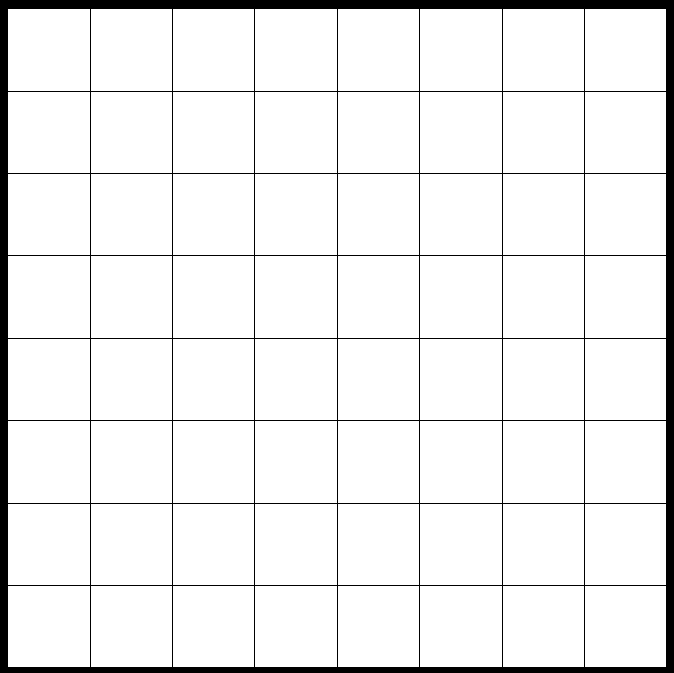
\includegraphics[width=2.8cm, height=2.8cm]{Fig1.png}
         \caption{Open}
         %\label{fig:y equals x}
     \end{subfigure}
     \quad
     \begin{subfigure}[b]{0.24\columnwidth}
         \centering
         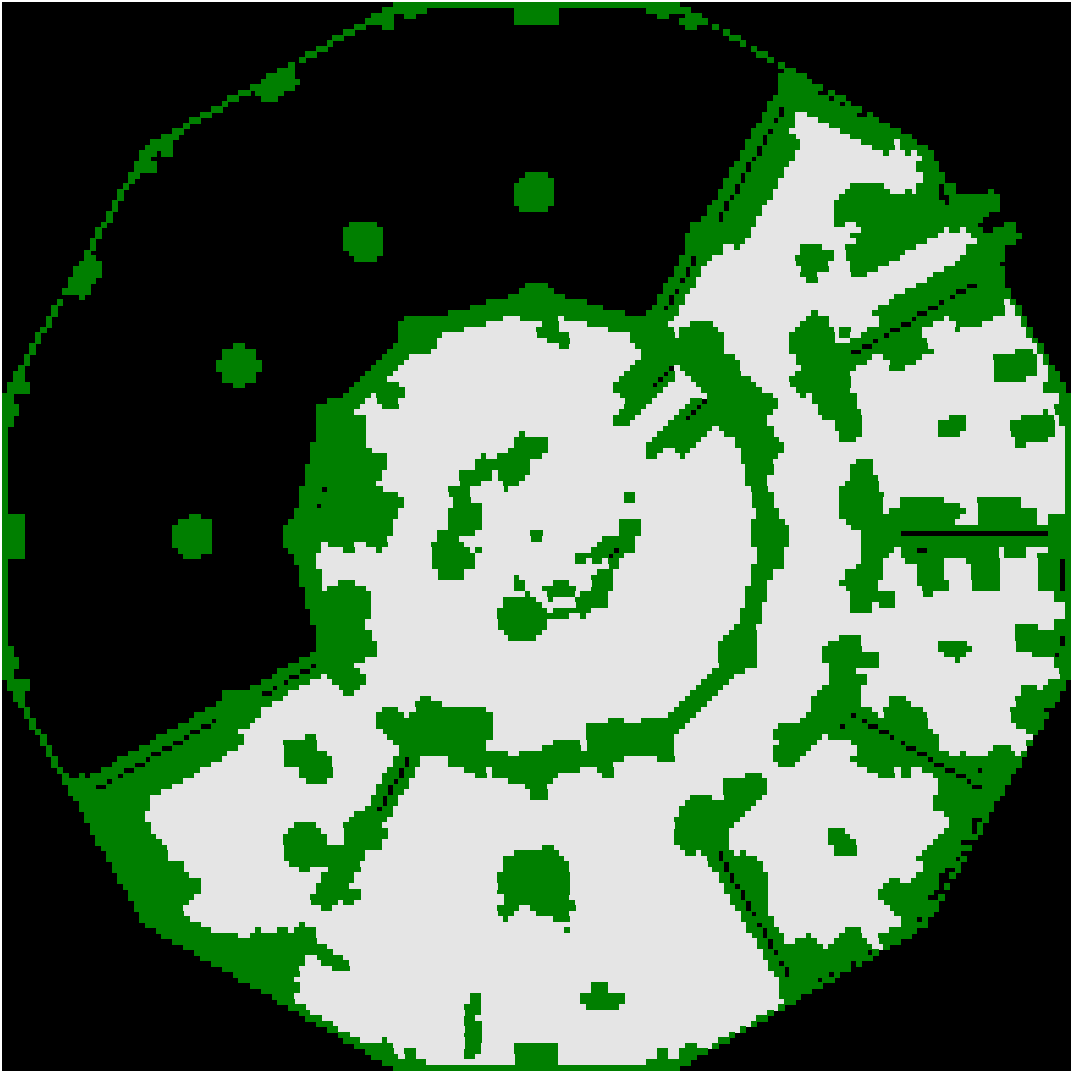
\includegraphics[width=2.8cm, height=2.8cm]{Fig2.png}
         \caption{DAO}
         %\label{fig:three sin x}
     \end{subfigure}
     \quad
     \begin{subfigure}[b]{0.4\columnwidth}
         \centering
         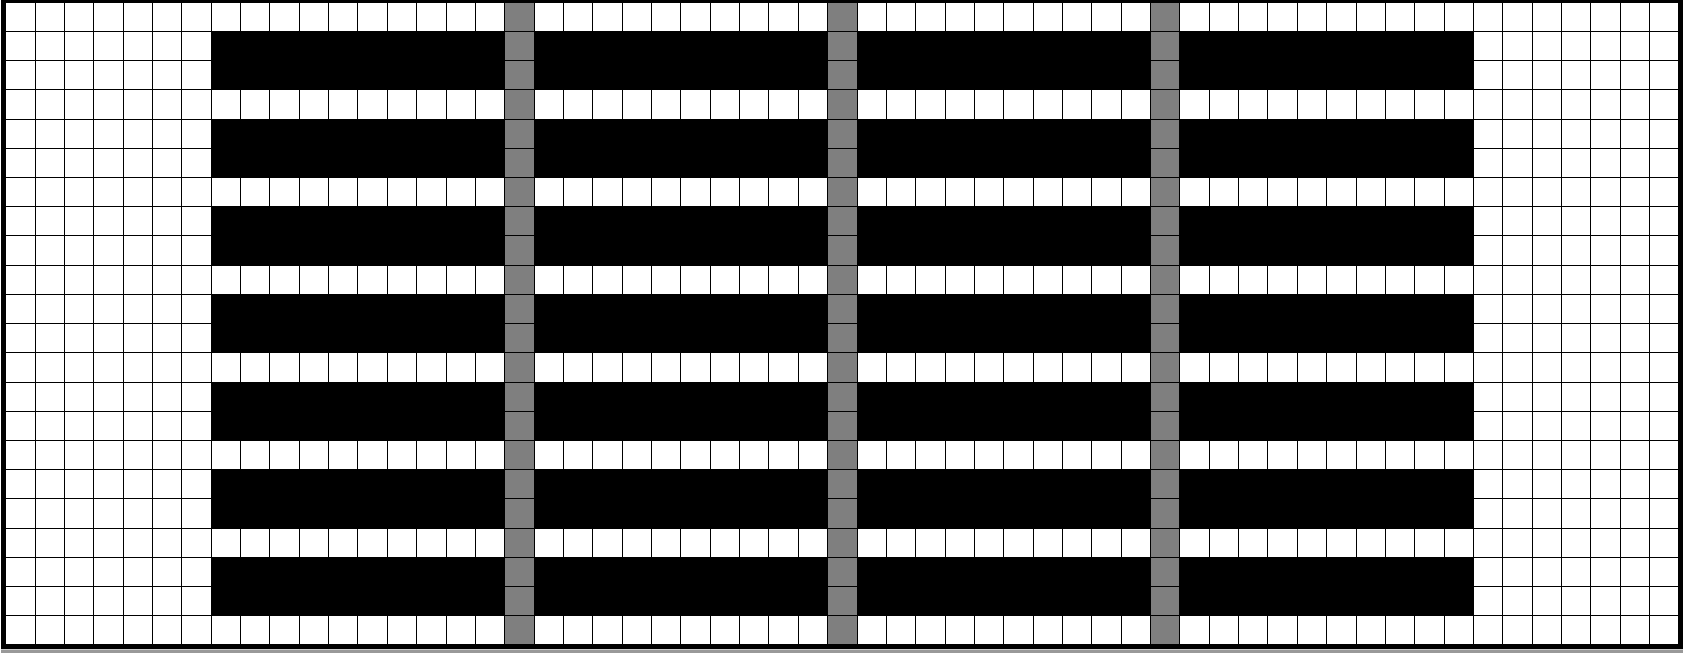
\includegraphics[width=6.2cm, height=2.8cm]{Fig3.png}
         \caption{Warehouse}% with \emph{PU}}
         %\label{fig:five over x}
     \end{subfigure}
        \caption{The Open (left), DAO (middle), and Warehouse (right) grids we used in our experiments. For the Warehouse grid, the gray cells mark the locations where uncertainty is introduced.}
        \label{fig:grid-types}
\end{figure}


All our experiments were performed over the following 4-neighborhood grids:
\begin{itemize}
    \item \textbf{Open.} An 8$\times$8 grid with no obstacles.
    \item \textbf{DAO.} A grid from the \texttt{ost003d} map of the game Dragon Age Origins (DAO), made publicly available by Sturtevant~\shortcite{sturtevant2012benchmarks}.
     \item \textbf{Warehouse.} A grid structured like an automated warehouse. 
     %A replica of this grid is a grocery store depicted in Figure~\ref{fig:Warehouse}.  
% \emph{Movements} are possible in empty cells as in Figure~\ref{fig:Warehouse}.  %     The third map we choose is Warehouse. 
% A replica of this map is a grocery store in which \emph{movements} are possible in empty cells as in Figure~\ref{fig:Warehouse}.
    %     a large circular map, from the game Dragon Age Origins (DAO), 
\end{itemize}
Figure~\ref{fig:grid-types} depicts these grids, where black cells and green cells are obstacles. 


% \roni{Tomer, can you create a figure with the 3 girds side-by-side?}
% We performed experiments in three differentan 8$\times$8 Open  and \texttt{ost003d}, a large circular map, from the game Dragon Age Origins (DAO), which is publicly available~\cite{sturtevant2012benchmarks}. 
% Both these maps are 4-connected in our experiments. 
% The third map we choose is Warehouse. 
% A replica of this map is a grocery store in which \emph{movements} are possible in empty cells as in Figure~\ref{fig:Warehouse}.  


% \begin{figure}[htp]
% \centering
% 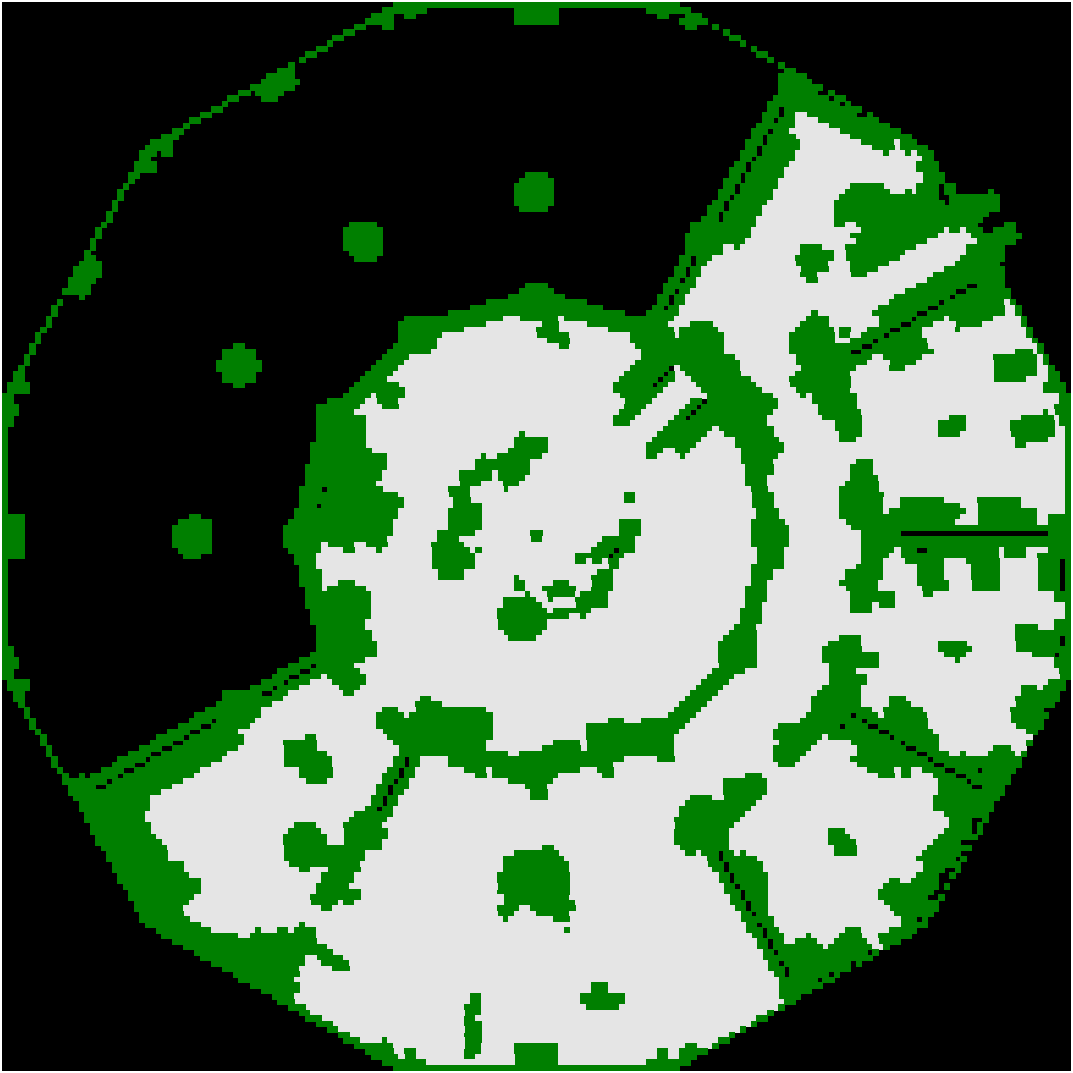
\includegraphics[width=.3\textwidth]{ost003d.png}\hfill
% % 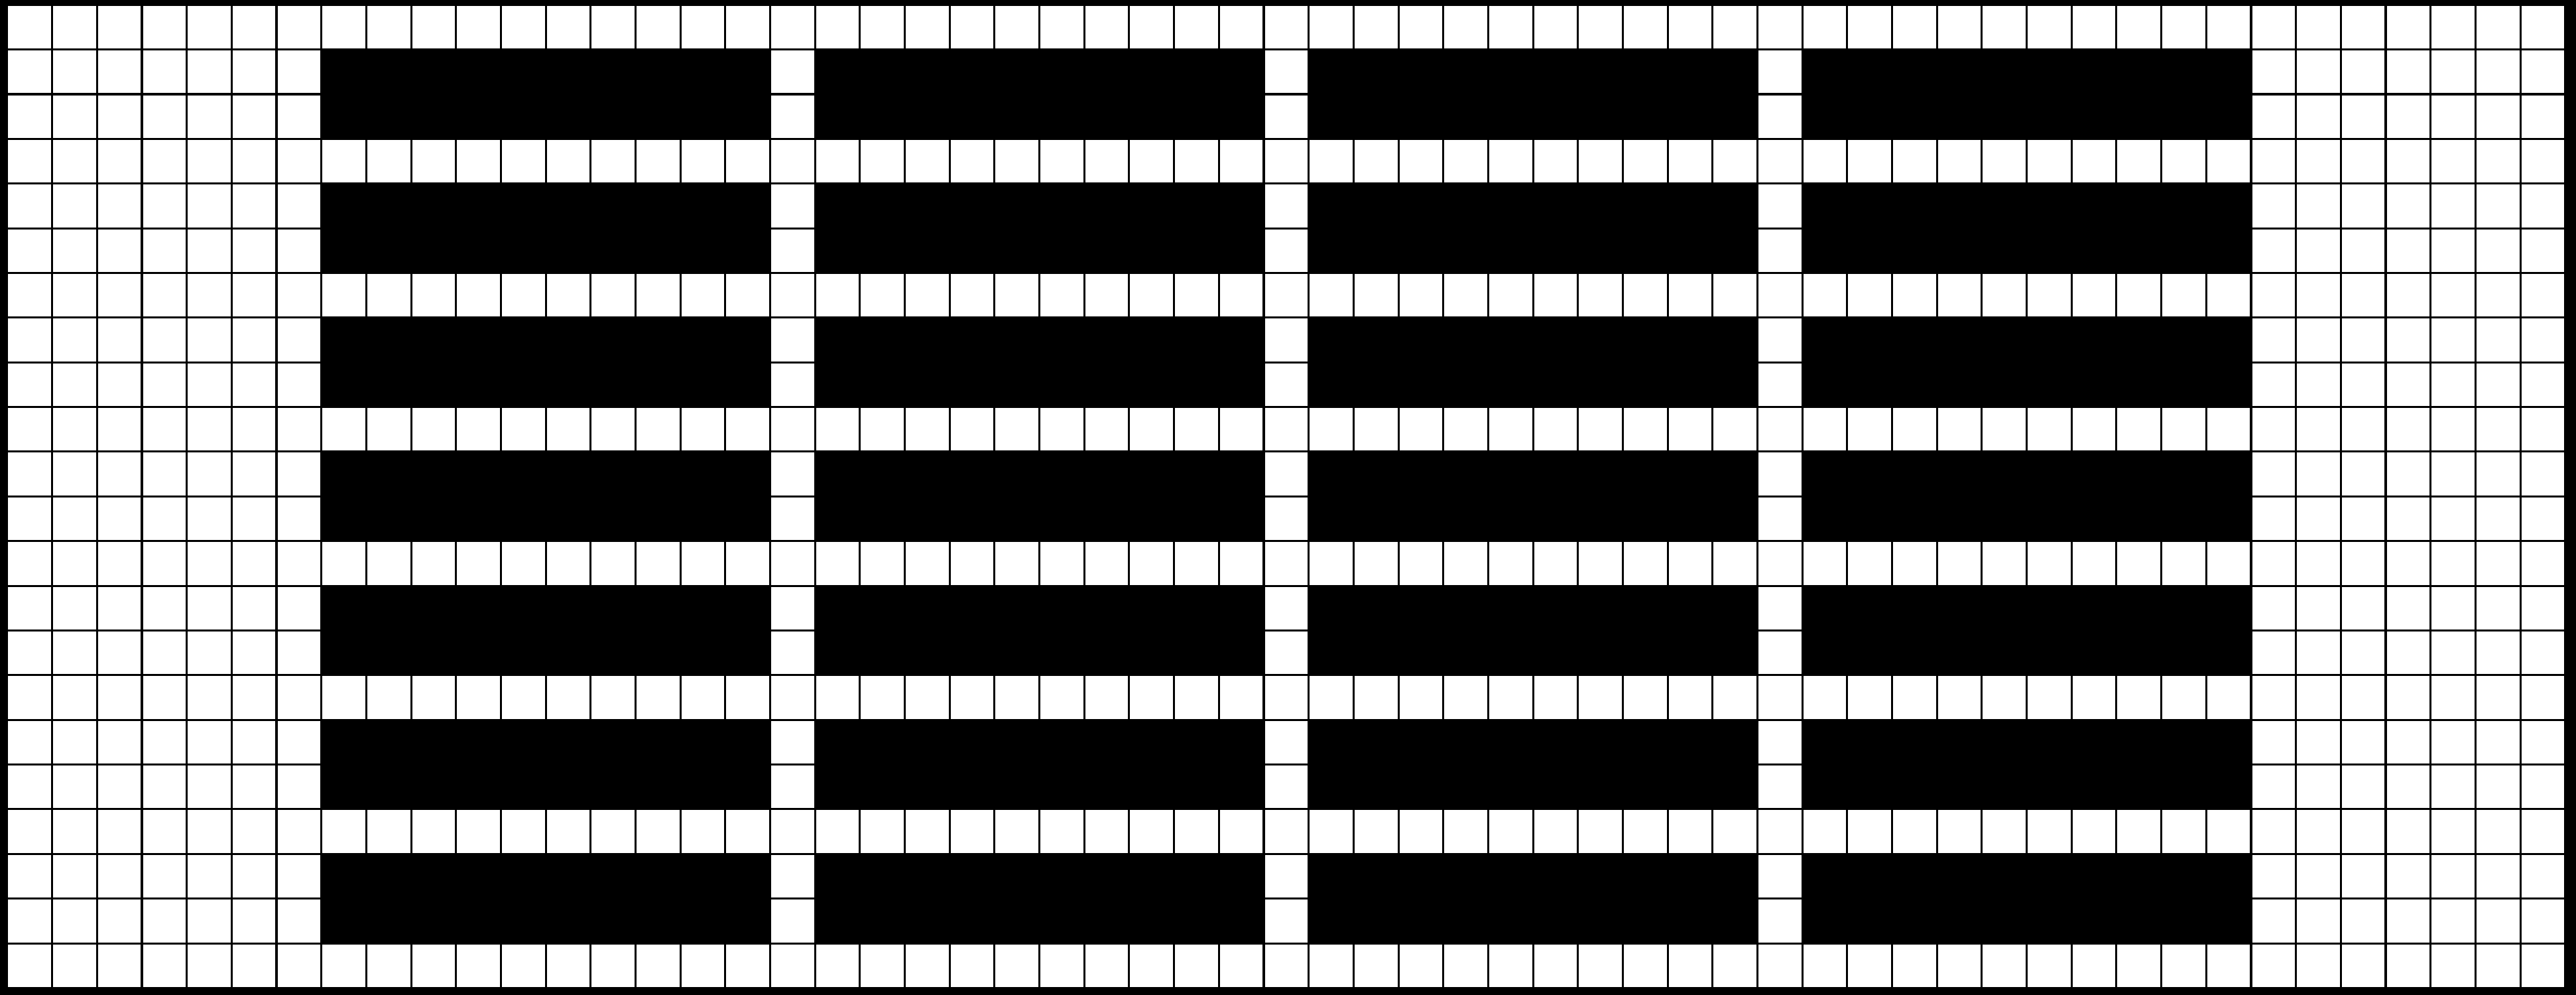
\includegraphics[width=.3\textwidth]{warehouse_FU.pdf}\hfill
% 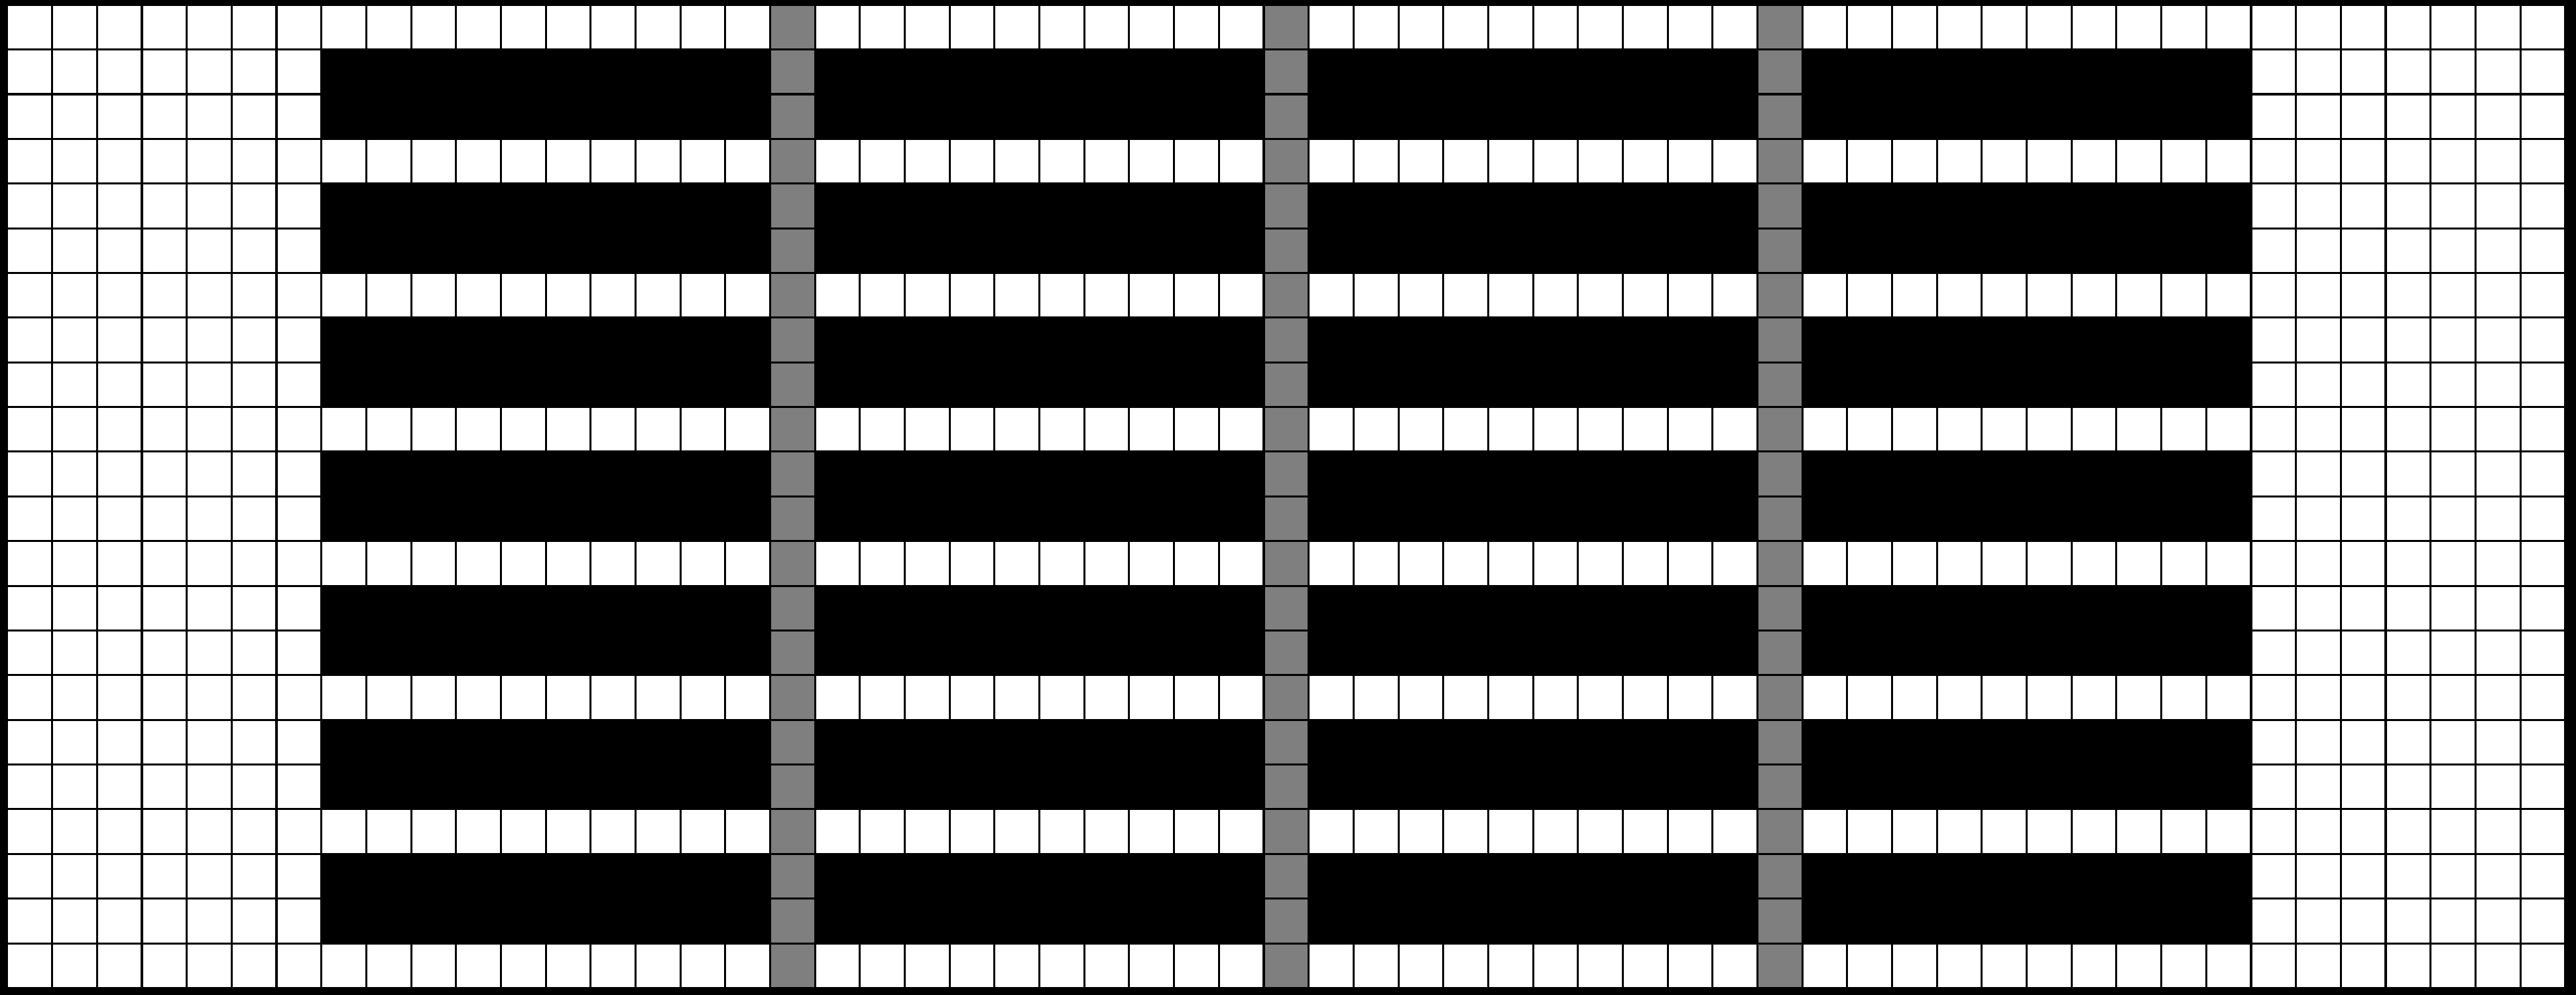
\includegraphics[width=.6\textwidth]{warehouse_PU.pdf}
% \caption{The maps used for the experiments. The figure on the left corresponds to the DAO map used, while the figure on the right is the warehouse map. For the setting with \textit{partial uncertainty}, only the areas colored in grey were assigned any uncertainty.}
% \label{fig:maps}
% \end{figure}


To define $\timel(e)$ and $\timeu(e)$ for every edge $e$ we introduce a parameter $U$ called the \emph{uncertainty rate}. For a given value of $U$, we set $\timel(e)$ to be a value chosen uniformly at random from the range $[1,U+1]$, 
and set $\timeu(e)$ to be a value chosen uniformly at random from the range $[\timel(e), U+1]$. 
Thus, the uncertainty rate parameter $U$ allows control over the amount of uncertainty in the generated experiment,  
where $U=0$ means no uncertainty. 
For each grid, we run experiments with an increasing number of agents, starting from 2 and going up to 20 agents. 
For each configuration of grid type, $U$, and number of agents, we created 50 experiments. 
These 50 experiments differ in the start and goal locations of the agents, which were randomly selected. 
We set a \emph{timeout} of \textbf{five minutes} for each solving each \mapftu instance. The \emph{success rate} of an algorithm is the ratio of problems solved before reaching this timeout. Unless stated otherwise, the objective function we optimized for was \socpes. 
%\roni{Tomer, please verify this really is the objective function used, we seem to say the opposite later} \tomer{Yeah its correct.}




The existing MAPF code frameworks that we explored were not easily adaptable to the \mapftu setting.
So, we implemented all algorithms from scratch, including the two CBS enhancements mentioned in Section~\ref{sec:cbs-enhancements}. 
%along with two CBS enhancement techniques.
As such, the performance of our algorithms is not directly comparable to state-of-the-art implementations of algorithms for classical MAPF, even when $U=0$, and scales less gracefully. 
Nevertheless, the source code for running all our experiments is publicly available at \texttt{https://github.com/Tomer-Shahar/Conformant-CBS}.
%\roni{Tomer, please have here a link to your code.}












% For every edge

% of $\timel(e)$ of every edge $e$ in the map, we set $\timel(e)$ to be a value chosen uniformly at random from the range $[1,1+U]$.


% When generating a \mapftu instance for a given value of $U$, we set the value of $\timel(e)$ of every edge $e$ in the map, we set $\timel(e)$ to be a value chosen uniformly at random from the range $[1,1+U]$.
% Then, we set $\timeu(e)$ to be a value chosen uniformly at random from the range $[\timel(e), 1+U]$. 
% Setting the uncertainty rate allows control over the amount of uncertainty in the generated experiment. 
% For each map, we run experiments with an increasing number of agents, from $k = 2$ up to 20 agents, and an uncertainty rate $U \in \{0, 1, 2, 4\}$. 
% To see the effect of uncertainty in each environment, we randomly select a $U$ for all the edges in the map.
% \roni{I am confused. $U$ is selected randomly from which range of values? Do you set $U$ to some number?}
% \shashank{U is an integer  selected randomly from \{0,1,2,4\}.}
% \roni{No this doesn't make sense, since in the results table we have U values in the columns. So, they are not selected randomly. }


\subsection{Experimental Results}



%When PC but no BP
\begin{table}
\resizebox{1\textwidth}{!}
{
\centering
{
\begin{tabular}{l*{8}{r}}
\toprule
$k$ & \multicolumn{2}{c}{$U = 0$} & \multicolumn{2}{c}{$U = 1$} & \multicolumn{2}{c}{$U = 2$} & \multicolumn{2}{c}{$U = 4$} \\
\cmidrule(lr){2-3}\cmidrule(lr){4-5}\cmidrule(lr){6-7}\cmidrule(lr){8-9}
 & \emph{\cbstu} & \emph{\odatu} & \emph{\cbstu} & \emph{\odatu} & \emph{\cbstu} & \emph{\odatu} & \emph{\cbstu} & \emph{\odatu} \\ \midrule
3   & 100\%  & 100\%   & 100\%  & 100\%   & 100\%  & 100\%   & 100\%  & 100\%   \\
7   & 100\%  & 100\%   & 100\%  & 88\%  & 94\%   & 72\%  & 58\%   & 46\%  \\
10  & 100\%  & 87\%  & 80\%   & 43\%  & 54\%   & 13\%  & 12\%   & 0\%  \\
15  & 100\%   & 13\%  & 18\%   & 3\%  & 0\%  & 0\%   & 0\%   & 0\%   \\ \bottomrule
\end{tabular}
}
}
\caption{Success rates results for \cbstu and \odatu algorithms on the Open grid.}
\label{tab:success-rate-1}
\end{table}

\begin{table}
\resizebox{1\textwidth}{!}{
\centering
{
\begin{tabular}{l*{8}{r}}
\toprule
$k$ & \multicolumn{2}{c}{$U = 0$} & \multicolumn{2}{c}{$U = 1$} & \multicolumn{2}{c}{$U = 2$} & \multicolumn{2}{c}{$U = 4$} \\
\cmidrule(lr){2-3}\cmidrule(lr){4-5}\cmidrule(lr){6-7}\cmidrule(lr){8-9}
 & \emph{\cbstu} & \emph{\odatu} & \emph{\cbstu} & \emph{\odatu} & \emph{\cbstu} & \emph{\odatu} & \emph{\cbstu} & \emph{\odatu} \\ \midrule
4   & 100\%  & 100\%   & 52\%   & 17\%  & 44\%   & 23\%  & 22\%   & 13\%  \\
7   & 92\%  & 93\%  & 14\%   & 0\%   & 2\%  & 0\%   & 0\%  & 0\%   \\
10  & 80\%   & 70\%  & 4\%  & 0\%   & 3\%  & 0\%   & 0\%  & 0\%   \\
13  & 70\%   & 27\%  & 0\%  & 0\%   & 0\%  & 0\%   & 0\%  & 0\%   \\
\bottomrule
\end{tabular}}
}
\caption{Success rates results for \cbstu and \odatu algorithms on the DAO grid.}
\label{tab:success-rate-2}
\end{table}



%
%Since prior work do not address time uncertainty, we implemented all algorithms from scratch %
%\Shashank{I guess we should mention this: As somehow reviewers from IJCAI had this issue why uncertainty bringing the life of \cbstu approach so down?We implemented our own version of vanilla CBS and ODA*, probably less efficient.  We can see that with 0 uncertainty (the usual MAPF problems), within the \emph{timebound}, CBS could solve instances up to 15 agents with success rate of 70\%.  Introducing uncertainty makes problems harder to solve. 
%\cbstu could solve problems up to 10 agents with 93\% and 67\% success rates, respectively for $U=1$ and $U=2$.}
%\roni{You are right, but I'm not sure how to say this in the text}

Table~\ref{tab:success-rate-1} and Table~\ref{tab:success-rate-2} show the success rates of \cbstu and \odatu for different values of $U$ and numbers of agents on the Open and DAO grids, respectively.
Rows correspond to different numbers of agents, and columns represent different $U$ values and algorithms.
Each inner cell contains success rates. 
%The columns CBS and ODA* refer to \cbstu and \odatu, respectively. 
%for each algorithm depending on the setting depicted by the number of agents and $U$. 


\begin{figure}[t]
  \centering
  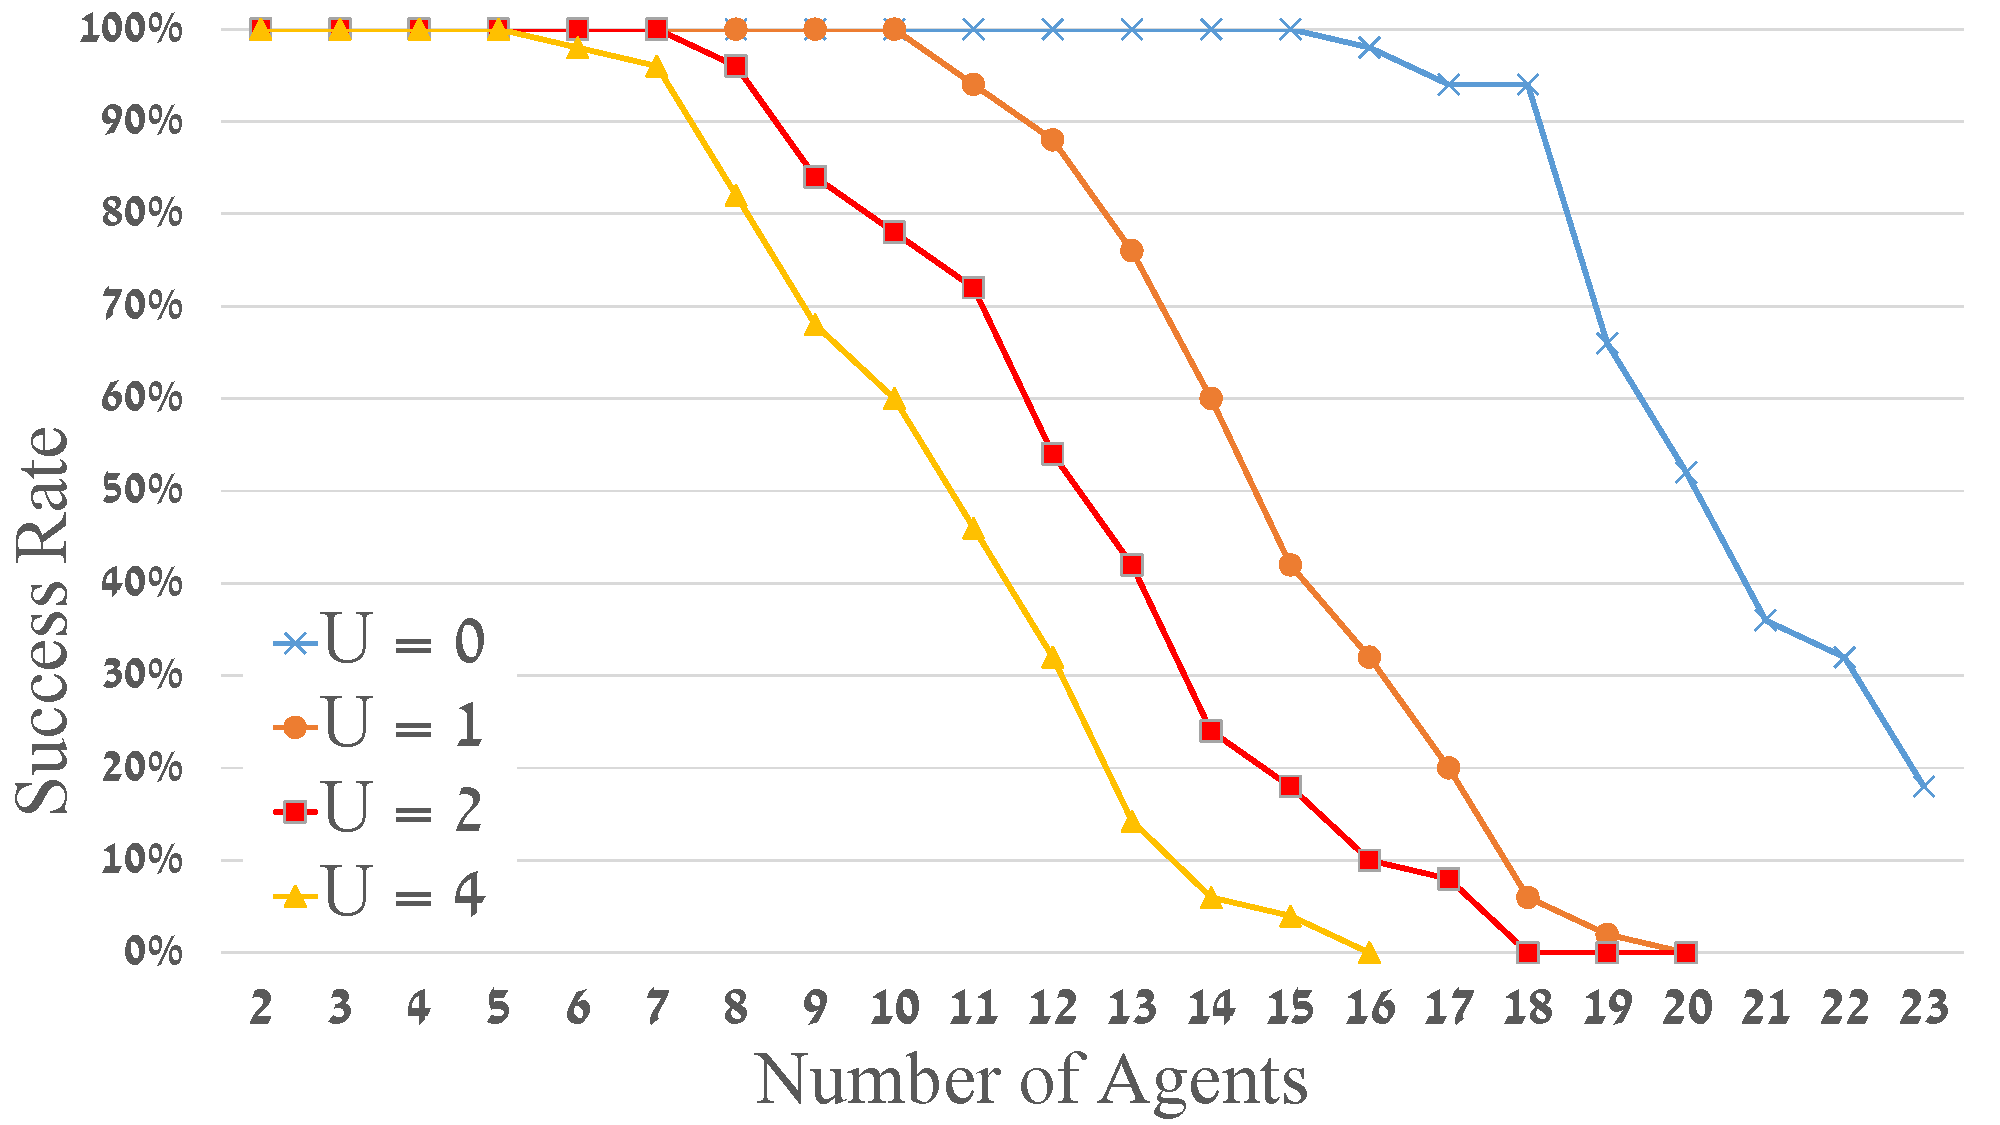
\includegraphics[width=0.8\columnwidth]{Figures/Success-vs_U.pdf}
  \caption{Success rates results for \cbstu on the Open grid.}
  %\roni{Tomer, can you increase the font in this figure? I can't read the x- and y-axis or the legend.}\tomer{Is this better?}} RONI: GOOD. The font is ugly, but, not important now
  \label{fig:cbs-success}
\end{figure}

We observe the following trends.
First, increasing $U$ significantly decreases the success rates of the algorithms.
For example, in the DAO grid with 7 agents, 
\cbstu solves all problem instances with $U=0$, but solves only 14\% for $U=1$. 
This trend is expected, as adding $U$ means more conflicts and a longer runtime to resolve new conflicts. 
Similarly, adding more agents makes problems harder for both algorithms, reducing the overall success rates. 
Another clear trend is that \cbstu outperforms \odatu for all the instances except for the case when 7 agents with $U=0$ on a DAO map. 
Indeed, CBS is also known to outperform \astar in classical MAPF on similar domains, 
and thus, the superior performance of its time uncertainty counter-part is expected. 
As \cbstu generally outperformed \odatu, we show results of only \cbstu hereinafter. 


Figure~\ref{fig:cbs-success} shows the success rate of \cbstu with more agents than in Table~\ref{tab:success-rate-1}. 
As expected adding more agents or increasing the uncertainty rate decreases the success rate. 
We note that \cbstu's performance when $U=0$ is similar to the performance of Improved CBS (ICBS) on a similar grid~\shortcite{BoyarskiFSSTBS15}.
% We see the impact of $U$ continues, especially when we compare it to the cases with no uncertainty.  
% We suspect this is because the single-agent plans contain ever increasing time intervals, which lead to many more potential conflicts which must be resolved one at a time. 
% Additionally, more time is needed to validate moves for both algorithms, and for the high-level approach of \cbstu, to perform goal tests. 
% \roni{This figure repeats the same results we have in the first table. What's the point???}\roni{I left it only to mention that ICBS performs the same}


%
\subsubsection{Sum of Costs Results}


% \begin{table}
% \centering
% %\resizebox{\columnwidth}{!}{
% \begin{tabular}{lrrrrr}
% \toprule
% \multirow{2}{*}{U}& \multicolumn{3}{c}{Sum of cost} & \multirow{2}[3]{*}{\shortstack{Time\\(secs)}} & \multirow{2}[3]{*}{\shortstack{Success\\Rate}} \\
% \cmidrule(lr){2-4}
%  & Min & Max & Range & \\
% \midrule
% 0  & 47.3  & 47.3  & 0.0   & 0.11 & 97\%   \\
% 1  & 64.9  & 80.6  & 15.8  & 2.41 & 86\%   \\
% 2  & 75.8  & 99.0  & 23.2  & 4.97 & 70\%   \\
% 4  & 94.0  & 145.5   & 51.5  & 5.26 & 50\%   \\ \bottomrule
% \end{tabular}
% %}
% \caption{Impact of uncertainty on the \emph{sum-of-cost}, \emph{time}, and \emph{success rate} of  \cbstu for 9 agents in $8\times 8$ Open Grid.}
%  \label{tab:8x8-cost-rate}
% \end{table}

%%This is the commented table with Exp data
% \begin{table}
% \centering
% %\resizebox{\columnwidth}{!}{
% \begin{tabular}{lrrrrrr}
% \toprule
% \multirow{2}{*}{$U$}& \multicolumn{3}{c}{\emph{Sum of Cost (SOC)}} & \multirow{2}[3]{*}{\shortstack{\emph{Time (secs)}}} &  \multirow{2}[3]{*}{\shortstack{\emph{Success Rate}}} & \multirow{2}[3]{*}{\shortstack{\emph{Exp}}} \\
% \cmidrule(lr){2-4}
%  & \emph{Min} & \emph{Max} & \emph{Range} & \\
% \midrule
% 0  & 48.8  & 48.8  & 0.0   & 0.04 & 100\% & 6.2   \\
% 1  & 60.7  & 71.74  & 11.04  & 2.33 & 100\%
% &34.9\\
% 2  & 73.52  & 97.05  & 23.52  & 5.79 & 86\%   &98.5 \\

% 3	&87.05	&123.03	&35.98 &11.44	&80\%	&175.3 \\

% 4  & 107.09  & 150.43   & 43.34  & 9.14 & 70\%   &199.7 \\
% 5	&108.07	&165.55	&57.48	&12.35	&58\% &406.3\\
% 6	&123.07	&178.97	&55.90	&18.68	&60\% &742.1\\
% 7	&138.74	&206.06	&67.32	&16.10	&68\% &-\\
% 8	&149.96	&238.39	&88.43	&21.56	&56\% &-
% \\
% \bottomrule
% \end{tabular}
% %}
% \caption{Impact of uncertainty on the \emph{sum-of-cost}, \emph{time}, and \emph{success rate} of  \cbstu for 9 agents in $8\times 8$ Open Grid. The objective is to \emph{minimize} the worst-case under the offline setting. $U$ is uncertainty and \textcolor{red}{$Exp$} is the number of nodes expanded in the high-level search tree.}
%  \label{tab:8x8-cost-rate}
% \end{table}


\begin{table}
\centering
%\resizebox{\columnwidth}{!}{
\begin{tabular}{lrrrrr}
\toprule
%\multirow{2}{*}{$U$}& \multicolumn{3}{c}{\emph{Sum of Cost (SOC)}} & \multirow{2}[3]{*}{\shortstack{\emph{Time}}} &  \multirow{2}[3]{*}{\shortstack{\emph{Success}}}  & \multirow{2}[3]{*}{\shortstack{\emph{Gen}}} \\
\multirow{2}{*}{$U$}& \multicolumn{3}{c}{\emph{Sum of Cost (SOC)}} & \multirow{2}[3]{*}{\shortstack{\emph{Time}}} &  \multirow{2}[3]{*}{\shortstack{\emph{Success}}}  \\
%& \multirow{2}[3]{*}{\shortstack{\emph{Gen}}} \\
\cmidrule(lr){2-4}
 & \emph{Opt.} & \emph{Pes.} & \emph{Range} & \\
\midrule
0  & 47.7  & 47.7  & 0.0   & 0.04 & 100\% \\ %& 10.9   \\
1  & 59.5  & 70.3  & 10.8  & 2.59 & 100\% \\ %&75.8\\
2  & 73.6  & 96.9  & 23.3  & 5.59 & 98\%   \\ %&869.6 \\ 

3	&86.4	&122.2	&35.8 &20.2	&84\%	\\ %&384.7 \\

4  & 104.0  & 146.7  & 42.7  & 19.4 & 70\%  \\ % &508.9 \\
5	&107.3	&166.0	&58.7	&34.3	&67\% \\ %&1066.7\\
6	&122.5	&179.4	&56.0	&30.1	&69\% \\ %&2071.3\\
7 &137.3	&205.2	&67.9	&23.9	&69\% \\ %&585.3\\
8 &145.9	&232.8	&86.9	&32.6	&53\% \\ %&888.8 \\
9 &171.5	&286.5	&115.0	&42.0	&50\% \\ %&2072.4 \\
\bottomrule
\end{tabular}
%}
\caption{\socopt, \socpes, runtime, and success rate results for Open grid with 9 agents.}% The objective is to \emph{minimize} the pessimistic bound under the offline setting. $U$ is the uncertainty rate.} %and \emph{Gen} is the number of nodes generated in the high-level search tree.}  
\label{tab:8x8-cost-rate}
\end{table}
%\roni{Tomer, please remove the Gen column from this table}done

To have a deeper understanding of the impact of $U$ on \cbstu's behavior, Table~\ref{tab:8x8-cost-rate} shows the results of experiments with a wider range of uncertainty rate values ($U$). 
These experiments were conducted on the Open grid with 9 agents. 
The table columns show 
the \socopt (the ``Opt.'' column), 
\socpes (``Pes.''), 
the difference between them (``Range''), 
the \cbstu computational runtime (``Time'') in seconds, 
and the success rate (``Success''). 


As seen in Tables~\ref{tab:success-rate-1} and~\ref{tab:success-rate-2}, increasing $U$ in general decreases the success rate. 
However, this relation between $U$ and success rate is noisy, indicating that the complexity of \mapftu is affected by other problem features as well. Similarly, the computational time does not fully correlate with $U$, but the general trend 
clearly indicates that higher uncertainty rate makes the problem, in general, harder to solve for \cbstu.  


Next, consider the difference between \socopt and \socpes (shown in the ``Range'' column), 
which we will refer to as the \emph{uncertainty range} of the solution. 
The results clearly show that the uncertainty range increases significantly with $U$. 
For example, the uncertainty range is 23.3, 42.7, and 86.9 for $U$=2, 4, and, 8, respectively. 
More generally, the results show that the uncertainty range increases linearly with $U$, with an increase of around 11 per $U$.
%and for $U=4$, the difference grows to 42.7. And, for the case when $U=8$, the difference becomes 86.9 with a success rate of 53\%. the sucess rate is not discussed!
Note that \cbstu and \odatu are both optimal and thus their solutions will have exactly the same \socpes. Their \socopt, however, can differ. 
While this is not reported these results, we have observed that both algorithms yielded solutions with \socpes that were almost identical for all the problems, and thus have almost identical uncertainty range.  
%\roni{Tomer, the original text is commented below. You say there that we optimized for \socopt but I think you said earlier that we optimized for \socpes. Which one is it?} \tomer{apologies, we optimized for \socpes in this section.}
%Note that \cbstu and \odatu are both optimal and thus their solutions will have exactly the same Opt. SOC. \roni{What are we optimizing in this experiment? I thought we said we were always optimizing the Pessimistic SOC? Tomer please check} The Pes. SOC, however, can differ, since we only aimed to optimize the optimistic SOC. While this is not reported in the table, we observed that both algorithms yielded Pes. SOCs that were almost identical for all the instances. 
% The uncertainty range of the final solution, i.e., the difference between Opt. SOC and Pes. SOC, increases linearly with $U$ with an increase of around 11 per $U$. We observed that the success rate indeed decreases with greater values of $U$, but not directly or even monotonically for that matter. 
%\roni{Ideally we will add some explanation of why this happens. I guess we don't have such an explanation}
% Up to $U=5$, the success rate steadily decreases but then appears to plateau for a while before further descending. 
% Note that the time column refers only to instances that were solved, thus it does not correlate directly with the success rate. However, the increase in time from $U=0$ to $U=1$ is evident, indicating that higher uncertainty rate makes the problem, in general, harder to solve for \cbstu.  


\subsubsection{Warehouse Results}

\begin{table}
\centering
{
\begin{tabular}{l*{8}{r}}
\toprule
$k$ & \multicolumn{2}{c}{$U = 0$} & \multicolumn{2}{c}{$U = 1$} & \multicolumn{2}{c}{$U = 2$} & \multicolumn{2}{c}{$U = 4$} \\
\cmidrule(lr){2-3}\cmidrule(lr){4-5}\cmidrule(lr){6-7}\cmidrule(lr){8-9}
  & \emph{CU} & \emph{PU} & \emph{CU} & \emph{PU} & \emph{CU} & \emph{PU} & \emph{CU} & \emph{PU} \\ \midrule
4   & 100\%	&100\%	&96\%	&100\%	&92\%	&98\%	&86\%	&96\%
\\
7   &98\%	&98\%	&84\%	&96\%	&68\%	&92\%	&48\%	&80\%
   \\
10  &94\%	&94\%	&48\%	&76\%	&34\%	&68\%	&10\%	&56\%
\\
13  &82\%	&82\%	&18\%	&42\%	&6\%	&28\%	&0\%	&18\%
\\
\bottomrule
\end{tabular}}
\caption{Success rates results for \cbstu on the Warehouse grid in the complete uncertainty (CU) 
%that choose to have uncertainty selected randomly, 
and the partial uncertainty (PU) experiment types.
%that chooses specific edges based on the structure of the map to have uncertainty.}
}
\label{tab:success-rate-3}
\end{table}

Finally, we present results for the Warehouse grid. 
Here we performed two types of experiments: 
\emph{Complete Uncertainty} (CU) and \emph{Partial Uncertainty} (PU).
CU experiments are the same as those described above.
PU experiments are different in that they introduce uncertainty only on a specific set of edges. 
These edges are marked in gray in Figure~\ref{fig:grid-types} (right). 
The motivation for PU experiments is to simulate automated warehouse scenarios, where most of the  uncertainty is condensed in specific areas such as the pickup depots and packaging areas. 
Obviously, experiments under PU and CU settings would be the same when $U=0$. 

Table~\ref{tab:success-rate-3} shows the success rate for different number of agents ($k$) and uncertainty rate ($U$). 
The results show that \cbstu performed better with PU than with CU in terms of the success rate. 
For example, 10 agents and $U=4$, \cbstu with PU received a success rate of 56\%, while \cbstu with CU received only a success rate of 10\%.  A similar trend was also observed on other grids. This is expected, since PU has strictly less uncertainty than CU. 


%\roni{These results make no sense. Why is the point of comparing CU and PU? they are not different algorithms. Of course CU will be harder to solve - it has strictly less uncertainty!! The point was to have larger U values since we're focusing them on small areas.}

%someintuition behind that is that, in a store as in Figure~\ref{fig:Warehouse}, the edge duration for an edge between two cells shown by a red dot is much more uncertain than for an edge between a cell connected to a cell shown by the green dot, seeing as those zones are both likely to have more traffic compared to the rest of the map and are prone to congestion which often leads to unpredictable delays. %\shashank{Roni, please see last 3-4 sentences about the partial U in warehouse map. Needs some rephrasing.}
%
%\dor{Maybe we can say here that it is also possible to set in $U$ a random number from a non-uniform distribution.}\roni{Not sure I followed}

% \shashank{Rewriting from "However, in contrast ..." \\
% However in warehouse maps, in contrast, we also keep time uncertainty over only a subset of edges, which means no time uncertainty over an edge not existing in this subset. The subset represents busier sections of a warehouse. 
% The intuition is that, in Figure~\ref{fig:Warehouse}, 
% the time it takes to cross a nearby region marked by "+" can be more uncertain than that of the top right corner. }





To summarize, we demonstrated that both \cbstu and \odatu can be applied to find safe and optimal solutions on real MAPF benchmarks. 
Increasing the uncertainty rate lowers the success rate and increases the SOC and uncertainty range of the returned solutions.  
If we compare the \cbstu and \odatu approaches, from the experiments we conducted, we observe that \cbstu performs significantly better.



\section{Safe Replanning}
\label{sensing}

%
% Explain that the agents may be able to sense their current location and time and react. 
% Key question: what to do with this information
%


% Sensing is something common. We consider it as well
In some scenarios, acting agents can \emph{sense} their environment, i.e., observe during the execution something that was unknown previously, and \emph{replan} based on their updated knowledge~\shortcite{SeukenZ2008}. 
In this section, we consider how sensing and online replanning can be useful in the context of \mapftu. 
The type of sensing we focus on is where an agent can sense the current time when it arrives at a vertex $v$. 
This eliminates the uncertainty embodied by the potential presence of that agent at $v$. Therefore, replanning at this stage may yield a better solution. 



In the rest of this section, we investigate two sensing and replanning settings. 
In the first, every agent attempts to improve its current single-agent plan individually while ensuring safety of the resulting overall solution.
In the second setting, the agents share sensing information with a central controller that may replan for multiple agents at once. % than in the no-communication setting.
We refer to the first setting as \sense and the second setting as \sensecom. 
In both settings, we assume that the agents are initially given a safe solution to the current \mapftu instance, computed offline using a \mapftu algorithm such as \cbstu or \odatu. 

For each setting, we provide theoretical examples showcasing the potential gains of  replanning and propose concrete replanning algorithms. 
Section~\ref{sensingResults} shows experimental results that measure the performance of these algorithms on \mapftu instances. The results confirm that our algorithms for \sense and \sensecom can result in executing a solution with a lower cost.

%, and that introducing online communications improves the overall performance even further.

 



% Specifically, we consider the setting where when an agent arrives at vertex $v$ it can sense the current time and its current location. This eliminates the uncertainty embodied by the potential presence of that agent at $v$. Therefore, replanning at this stage may yield a better solution. 



% We propose a simple approach to take advantage of potential sensing information. 
% First, we compute offline, a safe solution using a \mapftu algorithm such as \cbstu or \odatu. 
% $\pi_{i}$ is sent to each agent $a_i$ so that it can begin its execution. Then, when an agent senses the current time during execution, it may attempt to replan to exploit the sensed information while considering that the other agents are executing the safe solution. 
% Note that we assume here that agents can only sense when they arrive at a vertex. 

%so that it exploits the new information while considering the other agents' potential presences according $\Pi$. 
%We put one strong restriction that agents can sense successfully only when they arrive at a vertex. And if an agent succeeds, it can replan online without uncertainty regarding its current location and achieve a new solution, most likely a better one and with a lower cost. [repetition]


%In this section we describe online approaches to solve the MAPF-TU problem.
%These approaches use an offline solver, e.g., CBSTU, AODTU, as a subroutine with a few modifications.
%Since we have observed in Section~\ref{sec:xp-no-replanning} that CBSTU outperforms AODTU, we only adapt CBSTU to our online approaches. 
%However, in principle, this extension would work for any other MAPF-TU offline solver including AODTU.
%Our online approach is explained as follows: First an initial offline, safe solution is found using the CBSTU approach.
%Agents receive their paths and begin execution, and during the execution agents may sense their respective locations and current time.
%One restriction we assume that they can sense successfully only when they arrive at a vertex. 
%And if an agent succeeds, it can replan online without uncertainty regarding its current location and achieve a new solution, most likely a better one and with a lower cost. 

%Henceforth, we refer to the setting described in the previous section as sensing \emph{without} communication.

\subsection{The \sense Setting}
% Setting #1: agent may be able to sense their location and time sometimes.

%\subsubsection{Setting}
%We define sensing as follows: 
%Sensing is the ability of an agent to sense its current location during execution. [[repetition]]
% In this setting, when an agent executes its allocated single-agent plan ($\pi_{i}$) and arrives at vertex $v$, it may sense $v$ and the current time successfully. 
% This eliminates the uncertainty embodied by the potential presence of that agent at $v$. %regarding %its current location and the time it occupies the vertex $v$.
%\abda{these sentences are sloppy with regards to whether we sense location or time. See my long email from a few weeks back for why we should focus on sensing time.}\roni{did a quickfix}
%
%Formally, states of the agents will be derived from their potential presence. 
%
% Suppose in the initial plan, agent $a_i$ can occupy vertex $v$ between times $[t_1,t_2]$.
% Once execution begins, it can observe the current time $t\in[t_1,t_2]$, and be sure that it currently occupies $v$.  
% The agent can replan from $v$ (its new initial state) for itself, to its goal, and get a single-agent plan with a lower cost.
%The information obtained via sensing can lead to a better solution in terms of the overall cost. 
%Consider first a case where an agent can only know (sense) its own current location (a vertex along its allocated path). 
%Even with this restriction, the worst-case time can be improved considerably under certain conditions.



\begin{figure}[ht]
\centering
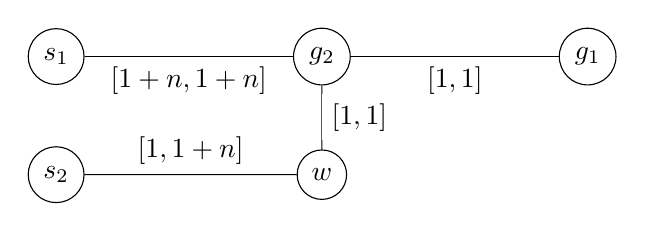
\begin{tikzpicture}[scale=0.75]
\tikzset{mapf-vertex/.style={circle, draw}}
\node[mapf-vertex] (s1) at (0.5, 0) {$s_1$};
\node[mapf-vertex] (s2) at (0.5, -2) {$s_2$};
\node[mapf-vertex] (t2) at (5, 0) {$g_2$};
\node[mapf-vertex] (t1) at (9.5, 0) {$g_1$};
\node[mapf-vertex] (w) at (5, -2) {$w$};
% \node at (8.5, -1.7) {$\sourcetargets = \tuple{(s_1, g_1), (s_2, g_2)}$};

\draw (s1) -- (t2) node [below,midway, fill=white] {$[1+n, 1+n]$};
\draw (t1) -- (t2) node [below,midway, fill=white] {$[1, 1]$};
\draw (w) -- (t2) node [right,midway, fill=white] {$[1, 1]$};
\draw (s2) -- (w) node [above,midway, fill=white] {$[1, 1+n]$};
\end{tikzpicture}

%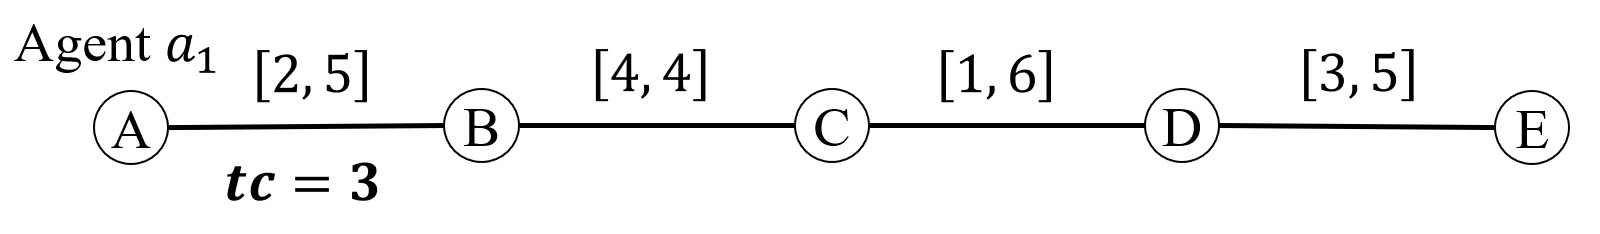
\includegraphics[width=\columnwidth]{fig-sensing-wo-com.jpg}
%\caption{Represents an \emph{offline} plan for agent $a_1$ where CBSTU minimized the worst-case. The original SOC range is $[12,22]$ for $a_1$ and the plan is: $A[0,0] \rightarrow B[2,5] \rightarrow B[3,6] \rightarrow B[4,7] \rightarrow C[8,11] \rightarrow D[9,17] \rightarrow E[12,22]$. It performs two \emph{wait} actions at vetex $B$.

\caption{MAPF-TU instance showing the benefits of replanning when \emph{sensing} might occur.
%The initial and goal vertices of the two agents are indicated in the bottom right.
Compared to the optimal, purely offline solution, the replanning solution decreases the pessimistic sum-of-costs from $4+3n$ to $4+2n$, when sensing actually occurs at vertex $w$.
}
\label{fig:sensing}
\end{figure}

The following example demonstrates the potential benefit of sensing in the \sense setting. 
\begin{example}
\label{ex:sensing-benefits}
Consider the \mapftu instance shown in Figure~\ref{fig:sensing}, 
and the solution comprising the single-agent plan  
$\big((s_1, g_2)(g_2, g_1)\big)$ for $a_1$ 
and the single-agent plan $\big((s_2, w) \dots (w, g_2)\big)$ 
for $a_2$, where the agent waits in $w$ for $n$ time steps. 
This solution is safe. 
Moreover, it is an optimal solution, in terms of both optimistic and pessimistic SOC (which are $4+2n$ and $4+3n$ respectively). 
However, if we allow replanning then when agent $a_2$ reaches vertex $w$ it can decide to reduce the amount of waiting based on how long it actually took to go from $s_2$ to $w$.
For example, assume that it took $n$ time steps for $a_2$ to reach $w$. 
Following the original safe solution, the agent would wait in $w$ for $n$ additional time steps before moving to $g_2$, reaching its goal at time $2n+1$. By sensing that it reached $w$ at time step $n$, the agent can reduce the planned wait time to a single time step, reaching its goal at time $n+2$. 
In general, through sensing and replanning optimistic and pessimistic SOC can be reduced down to $4+2n$ and $4+2n$, respectively. 
%here $tc$ represents the true-cost of the edge $AB$, i.e., $a_1$ senses this value after arriving at $B$ during execution. 
%
%$a_1$ replan by sensing (with $p=1$) that it arrived at $B$ at time $t=3$.
%After sensing, a low-level planner is called for $a_1$, but with the above described restrictions over the vertices and edges, and times it can occupy them in  future. 
%To make an online replanning approach produce an overall safe plan, $a_1$ could only occupy nodes $C, D$ and $E$ in times [8,11], [9,17], and [12,22] (allowed as per the original offline plan, especially because the central solver had the control), respectively. Similarly, edges $BC$, $CD$, $DE$ respectively at $[5,10]$, $[9,16]$, and $[10,21]$. 
%Suppose that even if the agent cannot sense in future from now on, the current online solution returned by the low-level solver would be 
%$B[3,3] \rightarrow B[4,4] \rightarrow C[8,8] \rightarrow D[9,14] \rightarrow E[12,19]$. Agent could save one \emph{wait}  at $B$ and the new maximum SOC is reduced to 19.  
\end{example}


\subsubsection{Replanning Algorithm}
We propose the following replanning algorithm for the \sense setting. 
Let $a_i$ be an agent following a single-agent plan $\pi_i$ that senses it has just reached vertex $v$ and the current time is $t$. 
Our replanning algorithm searches for the lowest-cost single-agent plan from $v$ to the goal of $a_i$, 
that is guaranteed to avoid conflicts with the other agents' execution of their single-agent plans. 
To this end, we restrict the new single-agent plan $\pi'_i$ such that the potential presences it induces 
are subsets of the potential presences induced by $\pi_i$. 
This means we can only choose to decrease the duration of its planned wait actions. 
Finding an optimal way to do this is a trivial---each agent simply waits until it reaches the lower time bound of its next non-wait action. 
% Address reviewer comment


\subsubsection{Theoretical Analysis}
%
%The advantage of sensing is the possibility of eliminating unnecessary \emph{wait} actions from the agent's plan.
%Typically, agents wait quite often during the execution, since the offline solution takes into account any possible combination of potential presence and provides a strong solution.
%
%\begin{proposition}
%Let $\Pi = (\pi_1, \dots, \pi_k)$ be the offline solution to a MAPF-TU instance.
%Assume that the path of agent $i$ is $\pi_i = v_0 \dots v_m \dots v_n$ and that $i$ replans after its $m^{\text{th}}$ move and obtain a new plan $v'_{m+1} \dots v'_{n'}$ from vertex $v_m$.
%Define $\pi' = v_0 \dots v_m v'_{m+1}\dots v'_{n'}$
%Let $\pi_i = v_0 \dots v_m \dots$ and if $v_{m+1} \dots$
%\end{proposition}
%

Let $\Pi$ be the \mapftu solution prior to replanning and let $\Pi'$ be the \mapftu solution after replanning. 
Since the potential presences according to $\Pi'$ are either the same or a subset of the potential presences in $\Pi$, 
the solution $\Pi'$ must be safe. 
%The approach generates constraints based on single-agent plans according to the time ranges in which the agents might occupy vertices and edges along their plans. Therefore, during subsequent replanning stages, an agent finds new moves only  along its own initial offline plan and will never conflict with the single-agent plans of other agents. 
Introducing replanning cannot lead to worse SOC bounds since the search space for each agent during replanning includes its original single-agent plan.
Thus, in the worst case the replanning will not change the current single-agent plan and $SOC(\Pi)=SOC(\Pi')$. %the overall SOC remains the same.
% During offline planning when two agents might collide, one of them will have to wait for several time steps, based on the conjunction of their \emph{potential presences} at a common vertex or edge. In order to provide an optimal, safe solution, all cases must be considered which might lead to time steps where an agent waits for no reason during execution. This is where sensing proves useful --- an agent can realize that some waiting moves can be skipped, as shown in  Example~\ref{ex:sensing-benefits}. Therefore, sensing is more useful when the single-agent plans obtained offline for agents are heavily intertwined and contain many \emph{wait} moves. [roni: all this is bla bla]
Since our replanning algorithm only removes wait actions, the best-case reduction in SOC (i.e., $SOC(\Pi)-SOC(\Pi')$) 
is bounded by the number of \emph{wait} moves in the offline solution.
%In the best case, sensing could reduce the SOC to the sum of the individual costs of the single-agent plans of all agents, if an agent plans without considering the presence of the other agents. \roni{This is an unsubstantiated claim. Do we have an example for this?}%Naturally, the benefits of sensing scale with the probability for agents to perform sensing.
%\roni{removed complexity section, it is super fast}

% \roni{The discussion about snapshot optimality is not convincing and not formal enough. I am removing it. See my comments in the commented text below for what is not clear}
%Due to the uncertainty of MAPF-TU, one cannot know in advance which solution has the actual lowest cost. \roni{what do you mean by actual lowest cost?}  Thus, when replanning, we can only choose the solution with the lowest cost, according to our current information. \roni{Lowest optimistic? pessimistic? actual?} A solution with this type of optimality is called a \emph{snapshot optimal} solution~\cite{vsvancara2019online}. \roni{Who says our replanning algorithm has this solution}
% Our approach considers all future uncertainty and always outputs an optimal, safe solution after every replanning stage, given that the initial offline plan is safe. Therefore, our approach is safe and snapshot optimal. %\dor{Is it snapshot optimal?}\roni{TODO DOR: Add a paragraph that explains what is snapshot optimal and how it carries to our context. Then say we are snapshot optimal}
%whom there was no worry for collision before, 
%but 

%This is verified by the positive constraints in $C_i$ 
%, even in the best case 
%(taken from the initial plan). 
%that guarantees that agents will never collide with each other.


\subsection{The \sensecom Setting}

%We define communication as so: 

%\roni{This is defined already above}
%Consider the case where the agents can also communicate with a central controller during execution. That is, when an agent $a_i$ senses its arrival time at a vertex $v$, it immediately shares this information with this central controller. That controller can then replan for all agents that are currently at a vertex (as opposed to at an edge) and send new single-agent plans back to these agents. Note that, we assume that this is an \emph{immediate act}, which happens in negligible time and hence the agents start to execute their new single-agent plans immediately.

%from same time point.  
%We do not take into consideration the time it takes for the sensing-sending-replanning part as this small amount of data transfer is negligible in real world scenarios where it occurs nearly instantaneously. 
\begin{figure}[ht]
\centering
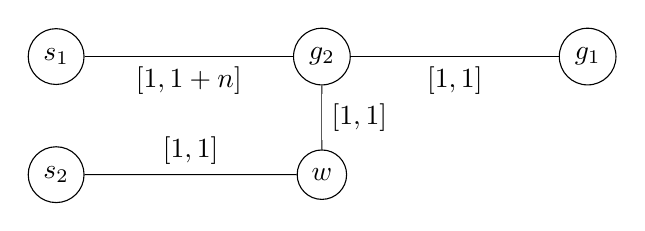
\begin{tikzpicture}[scale=0.75]
\tikzset{mapf-vertex/.style={circle, draw}}
\node[mapf-vertex] (s1) at (0.5, 0) {$s_1$};
\node[mapf-vertex] (s2) at (0.5, -2) {$s_2$};
\node[mapf-vertex] (t2) at (5, 0) {$g_2$};
\node[mapf-vertex] (t1) at (9.5, 0) {$g_1$};
\node[mapf-vertex] (w) at (5, -2) {$w$};
% \node at (8.5, -1.7) {$\sourcetargets = \tuple{(s_1, g_1), (s_2, g_2)}$};

\draw (s1) -- (t2) node [below,midway, fill=white] {$[1, 1+n]$};
\draw (s2) -- (w) node [above,midway, fill=white] {$[1, 1]$};
\draw (t1) -- (t2) node [below,midway, fill=white] {$[1, 1]$};
\draw (w) -- (t2) node [right,midway, fill=white] {$[1, 1]$};
\end{tikzpicture}

%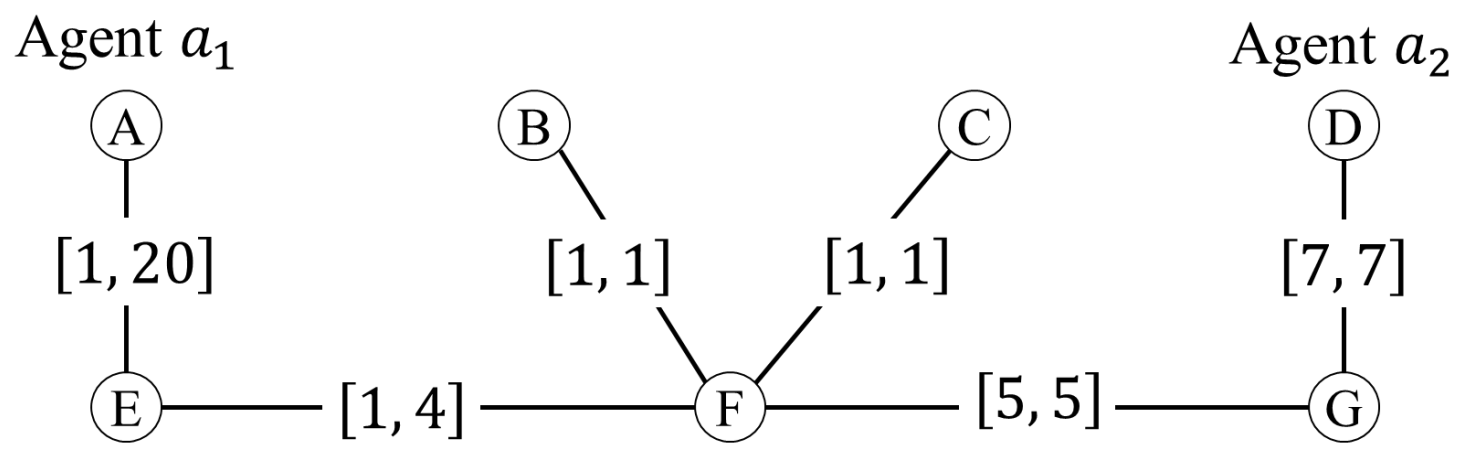
\includegraphics[width=\columnwidth]{no-comm-ex.png}
\caption{
\mapftu instance showing the benefits of replanning when sensing and \emph{communication} might occur.
%The initial and goal vertices of the two agents are indicated in the bottom right.
Compared to the optimal, purely offline solution, the replanning solution decreases the optimistic SOC from $4+n$ to $4$, when sensing occurs by agent $a_1$ in vertex $g_2$.}
%Agents $1$ and $2$ start from vertices $s_1$ and $s_2$ and their goals are the vertices $t_1$ and $t_2$, respectively.}
\label{fig:communications-benefit}
\end{figure}

In the \sensecom setting, agents share the information they sensed. 
This sharing occurs when an agent reaches a vertex and it is able to sense. 
Thus, the input to replanning here is a set of agents that arrived at a vertex at the same time and were able to sense. We call this set of agents the \emph{replanning agents}. 
The following example demonstrates the potential benefit of sensing in the \sensecom setting, showing that this setting allows further reduction in SOC over what is possible in the \sense setting.  
\begin{example}
Consider the \mapftu instance shown in Figure~\ref{fig:communications-benefit}, 
and the solution comprising the single-agent plan  
$\big((s_1, g_2)(g_2, g_1)\big)$ for $a_1$ 
and the single-agent plan $\big((s_2, w) \dots (w, g_2)\big)$ 
for $a_2$, where the agent waits in $w$ for $n$ time steps. 
This solution is safe and optimal in terms of SOC (the pessimistic and optimistic SOC is $4+n$ and $4+2n$, respectively). 

However, if we allow replanning and communications, and if agent $a_1$ senses when reaching vertex $g_2$ and broadcasts its arrival time, then agent $a_2$ can decide to reduce the amount of waiting based on how long it took going from $s_1$ to $g_2$.
In the optimal case where agent $a_1$ reaches $g_2$ at time $1$, the SOC range for the replanning approach is $[4, 4+2n]$. %\dor{It seems more reasonable for agent $a_1$ to wait only 2 steps instead of agent $a_2$ that waits $n$ steps, isn't it?}
%\shashank{appears okay to me... but I might be wrong. g2 is the goal for a2?}
%\tomer{I think the example is fine - Agent 2 is the one that has to wait since its goal obstructs Agent 1's only path. So agent 1 tries to cross g2 first and only then agent 2 can move.}
%Agent $a_1$ is travelling from vertex $A$ to $B$ while agent $a_2$ is travelling from $D$ to $C$. $a_1$ will occupy vertex $F$ between $t\in[2, 24]$ while $a_2$ will occupy it between $t\in[12, 12]$. There will be a potential collision at time $12$. 
%If $a_2$ occupies vertex $F$ first, and $a_2$ waits for $11$ time steps, the SOC will be $[27, 49]$. In contrast to that if $a_1$ traverses first then SOC will be $[29, 51]$. 
%Agent $a_1$ must wait for $11$ time steps or else it might reach $F$ at $t=12$, which leads to a collision. 
%However, if $a_1$ moves to $E$ and senses that its current state is $(E, 1)$, it can continue traversing along its path, reach $F$ at $t\in[2, 5]$. This does not violate the constraint of $(a_1, F, 12)$. The SOC will be $[16, 19]$ as we eliminated the inessential waiting times. 
%Note that if sensing is not allowed and $a_1$ arrives in $E$ at $t=1$, the SOC would be $[27, 30]$ because it needs to wait for next 11 time steps.
\end{example}

\subsubsection{Replanning Algorithm}



We propose to use \cbstu to generate a solution for the replanning agents that takes them from their current locations to their respective goal locations.  
To maintain safety, we initialize \cbstu with a set of \cbstu constraints that cover every potential presences of every agent that is not a replanning agent. This ensures that the agents with new single-agent plans will never conflict with agents that have not sensed.  
This is true even when the replanning phase assigns the agents a completely different solution to execute. This is why communication adds a facet of flexibility to replanning. 
%The potential presences of all sensing agents will be updated to reflect their current states. 
%This allows the planner to draw information from agents even if they never sense again in the future. %Add an example?.




% a replanning algorithm must avoid occupying the potential presences of any agent that is not currently replanning. 


% , but only allow these agents to replan. 
% T, since other agents  agent. 
% In our implementation, we used CBSTU for this purpose. The main reason for this is that an agent does not know whether it would sense in future after current replanning, and hence to make its single-agent plan safe, we need to consider the future time uncertainty. 
% %
% It is also not necessary that all the agents will sense at a given clock tick.
% Based on who sensed and communicated, the solver builds a new set of constraints based on the single-agent plans of those agents who have not sensed at this particular clock-tick. 

% The planner then creates a new solution for the agents who sensed, that takes them from their current locations to their respective goal locations, safely, even if no sensing happens further while taking into account the constraints generated earlier from the agents who are not sensing. 


\subsubsection{Theoretical Analysis}

Let $\Pi$ be the \mapftu solution prior to replanning, 
$\Pi_{WOC}$ be the \mapftu solution created after replanning under the \sense setting, 
and $\Pi_{WC}$ be the \mapftu solution created after replanning under the \sensecom setting. 
The ability to communicate expands the set of single-agent plans that may be assigned to the replanning agents. 
Thus, 
\begin{equation}
    SOC(\Pi)\geq SOC(\Pi_{WOC})\geq SOC(\Pi_{WC})
    \label{eq:ineq}
\end{equation} 
for the SOC being optimized (pessimistic or optimistic). 
Note, that $SOC(\Pi)$ is the SOC of the plan $\Pi$, as oppose to the cost of executing $\Pi$. 
For example, it may be that SOC($\Pi$)=10 but executing $\Pi$ would cost more. 
Thus, Equation~\ref{eq:ineq} does not mean executing $\Pi$ will necessarily cost more than executing $\Pi_{WOC}$, and 
that executing $\Pi_{WC}$ will necessarily cost less than $\Pi_{WOC}$. 
%During execution, further replanning may occur and the actual durations it take to pass each edge may vary such that 
%\shashank{last inequality does not hold?} % \roni{I changed the text, now Ok?}
% \shashank{May be the expectations of SOC would hold. As I discussed with Tomer  (Figure 7 shows that too), it's hard to relate them for a specific instance. The same is evident from the Table 5 and Table 6}
%\roni{I modified the text - is it more clear now?}
%This may lead to great gains as 
% The agents may suddenly follow substantially different plans, most likely better ones, leading to a fair gain in overall SOC. roni: repetition
% Even in the pessimistic scenario, it guarantees that the SOC will never exceed that of the non-communication variant.
%as the paths found when not communicating are included in the search space and thus will be considered as well. 
%Since the non-communication variant cannot perform worse than a complete offline solution and communication cannot increase the solution cost, this variation can only find a solution that has lower optimistic or pessimistic case SOC (depending on what we optimize). Note, however, that during execution of the remainder of the solution, the actual SOC may vary unexpectedly in this range. Roni: not sure what this means. Can the bounds change?
%improve the best and worse case SOC upon the initial SOC or maintain the same value.
%\dor{But we can see experimentally that the communication can decrease the cost.}[[You're right, it may have bad luck. Explained]


%\textcolor{red}{@Tomer, Time complexity needs to be rephrased }
\paragraph{Time complexity} Since this variant uses a centralized planner, the runtime of every replanning step is in the worst-case exponential in the number of replanning agents. 
However, the overall computation time is typically dominated by the time it takes to compute the initial solution since it always takes into consideration all the agents simultaneously with maximal uncertainty.
At a certain time-step, even if all the agents were to sense and replan simultaneously sometime during the execution, this would still be a considerably easier \mapftu instance to solve compared to the initial, offline solution that was already found. 
This is because much of the time uncertainty is removed from the solution up to this point leading to fewer potential conflicts over shorter time intervals across the entire solution.
Indeed, we observed in our experiments that all subsequent replanning stages were on an average several times faster than the time required to compute the initial solution.

\paragraph{Safety}  
%\tomer{Added a more detailed explanation.}
The output of each replanning stage is guaranteed to be safe. This occurs because whenever replanning happens, each agent either sensed (and subsequently replans) or it did not sense (since it is currently traveling or did not sense for any other reason). For all agents that did not sense, their current single-agent plans are treated as constraints for all the agents that will replan. Then, the central planner computes new single-agent plans for the sensing agents, using a \emph{safe} \mapftu algorithm. Since the other agents are taken into account through constraints, and a safe \mapftu solver is used, the solution found is guaranteed to contain no collisions in the future. Thus, the output for each replanning stage is a safe \mapftu solution.

%because the online planning algorithm treats the planned potential presences of the agents that have not sensed as constraints that are applied to all replanning agents. Thus they will never collide with their current respective plans.\dor{I couldn't understand the last sentence.}\roni{TODO DOR: This is intended to ``prove'' that it is safe. Please improve} And since a safe MAPF-TU algorithm is used, we ensure there are no conflicts among the agents who are receiving a new plan.

%
%It applies the constraints on the  agents who participate in replanning. This means that in future an agent will never collide with other agents. It is true since among the agents who have sensed, a regular optimal, safe offline plan is found centrally using CBSTU, which ensures zero conflict. \abda{rewrite this paragraph so that it also applies to aodtu and other solvers. Offline AODTU already has to deal with constraints, so no reason not to consider it applicable here.}





\section{Empirical Evaluation: Online Replanning}
\label{sensingResults}


% Experimental setup
In this section, we experimentally evaluate the benefit of using our online replanning algorithms for the \sense and \sensecom setting. 
%We assumed a complete sensing setup, i.e., whenever an agent finishes to traverse an edge, it senses its current location and time, and runs the appropriate replanning algorithm. 
We performed a range of experiments and report here only a representative subset of them. 
Specifically, we report here the results only for the Open grid and for the Warehouse grid with partial uncertainty (PU). 
In each experiment, we first obtained an initial safe solution using \cbstu. 
Then, we simulated the execution of this solution by sampling uniformly the edges' durations within their ranges. 
Whenever an agent finishes traversing an edge, it applies the appropriate replanning algorithm. 
Two types of experiments were performed, one where the objective is to minimize \socopt and one where the objective is to minimize \socpes.  
The main performance metric we consider here is the \emph{Final SOC} which is the SOC (either \socopt or \socpes) of the solution the agents ended up executing, following all the performed replanning. 


%We denote the SOC of the simulated execution of the initial safe solution by \emph{Final SOC}.


\subsection{Results for the Open grid}
\begin{table}
\parbox{.5\linewidth}{
\centering
\begin{tabular}{crrr}
\hline
\multirow{2}{*}{\textit{U}} & \multirow{2}{*}{\textit{Initial SOC}} & \multicolumn{2}{c}{\textit{Final SOC}} \\ \cline{3-4} 
 &  & \textit{\sense} & \textit{S+C} \\ \hline
0 & 43.06 & 43.06 & 43.06 \\
1 & 59.32 & 58.22 & 58.05 \\
2 & 72.89 & 72.61 & 72.96 \\
3 & 93.45 & 90.79 & 91.10 \\
4 & 111.09 & 109.10 & 107.64 \\
5 & 115.60 & 118.67 & 111.07 \\
6 & 129.53 & 137.96 & 127.33 \\
7 & 155.57 & 150.10 & 148.57 \\
8 & 166.89 & 163.47 & 159.22 \\ \hline
\end{tabular}
}
\hfill
\parbox{.5\linewidth}{
\centering
\begin{tabular}{crrr}
\hline
\multirow{2}{*}{\textit{U}} & \multirow{2}{*}{\textit{Initial SOC}} & \multicolumn{2}{c}{\textit{Final SOC}} \\ \cline{3-4} 
 &  & \multicolumn{1}{r}{\textit{\sense}} & \multicolumn{1}{r}{\textit{S+C}} \\ \hline
0 & 43.06 & 43.06 & 43.06 \\
1 & 58.58 & 58.16 & 58.63 \\
2 & 74.44 & 75.70 & 73.56 \\
3 & 93.76 & 92.74 & 91.88 \\
4 & 116.04 & 116.41 & 114.13 \\
5 & 124.07 & 125.02 & 120.04 \\
6 & 137.63 & 138.90 & 134.60 \\
7 & 163.10 & 158.98 & 160.68 \\
8 & 176.07 & 173.42 & 173.81 \\ \hline
\end{tabular}
}
\caption{Initial and Final SOC results for 8 agents in the Open grid, for the \sense and \sensecom (S+C) settings. 
The left side shows results for \socopt and the right side shows results for \socpes.}
\label{tab:open_map-absolute-online}
\end{table}


Table~\ref{tab:open_map-absolute-online} shows the Final SOC results for 8 agents in the Open Grid when optimizing for \socopt (left) and for \socpes (right). 
The \emph{Initial SOC} is the SOC (either \socopt or \socpes) of the initial solution. 
The \sense and S+C columns represent the \sense and \sensecom settings, respectively. 
Each line corresponds to a different uncertainty rates ($U=0,1,\dots,8$).
Every data cell is an average over 50 problem instances. 
Note that increasing $U$ inherently increases the SOC since it increases the edge traversal duration.
% For reviewer

%The results show the following trends.
The results in Table~\ref{tab:open_map-absolute-online} show that online replanning in this set of experiments is only marginally beneficial. 
This can be seen when comparing the Final SOC with the Initial SOC---if they are the same then there is no benefit to online replanning. 
The largest difference between the average Final SOC and Initial SOC is for $U=7$ in the \sense setting (150.10 Final SOC vs. 155.57 Initial SOC) and for $U=8$ in the \sensecom setting (159.22 Final SOC vs. 166.89 Initial SOC). 
In almost all cases, the Final SOC when in the \sensecom setting is smaller than the Final SOC in the \sense setting, which supports our theoretical analysis in the previous section. 



\begin{table}
\parbox{.5\linewidth}{
\centering
\begin{tabular}{c|rrrr}
 \hline
\textit{Agents} & \multicolumn{1}{c}{\textit{U=1}} & \multicolumn{1}{c}{\textit{U=2}} & \multicolumn{1}{c}{\textit{U=3}} & \multicolumn{1}{c}{\textit{U=4}} \\ \hline
\textit{2} & 11\% & 9\% & 12\% & 17\% \\
\textit{3} & 11\% & 9\% & 11\% & 15\% \\
\textit{4} & 9\% & 9\% & 10\% & 14\% \\
\textit{5} & 8\% & 8\% & 9\% & 13\% \\
\textit{6} & 7\% & 7\% & 9\% & 11\% \\
\textit{7} & 7\% & 8\% & 9\% & 9\% \\
\textit{8} & 6\% & 7\% & 9\% & 10\% \\
\textit{9} & 6\% & 7\% & 9\% & - \\
\textit{10} & 5\% & 7\% & 9\% & - \\
\textit{11} & 4\% & - & - & - \\
\textit{12} & 4\% & - & - & -  \\\hline
\end{tabular}
}
\hfill
\parbox{.5\linewidth}{
\centering
\begin{tabular}{c|rrrr}
 \hline
\textit{Agents} & \multicolumn{1}{c}{\textit{U=1}} & \multicolumn{1}{c}{\textit{U=2}} & \multicolumn{1}{c}{\textit{U=3}} & \multicolumn{1}{c}{\textit{U=4}} \\ \hline
\textit{2} & 0\% & 0\% & 0\% & 0\% \\
\textit{3} & 0\% & 0\% & 0\% & 1\% \\
\textit{4} & 0\% & 0\% & 0\% & 0\% \\
\textit{5} & 0\% & 0\% & 1\% & 1\% \\
\textit{6} & 0\% & 1\% & 1\% & 2\% \\
\textit{7} & 0\% & 2\% & 1\% & 2\% \\
\textit{8} & 0\% & 1\% & 2\% & 2\% \\
\textit{9} & 0\% & 2\% & 2\% & 3\% \\
\textit{10} & 0\% & 2\% & 2\% & 2\% \\
\textit{11} & 1\% & 1\% & 1\% & 2\% \\
\textit{12} & 1\% & 1\% & 1\% & 1\% \\ \hline
\end{tabular}
}
\caption{Overall SOC reduction, \sensecom setting, Open grid. 
(left) Results for optimizing \socopt, (right) Results for optimizing \socpes.}
\label{tab:open_map-percentage-online}
\end{table}

                                                              Next, we focus on the \sensecom setting and consider the impact of changing the number of agents on the ratio between the Final SOC and the Initial SOC. We refer to this ratio as the \emph{reduction in SOC} due to online replanning. 
Table~\ref{tab:open_map-percentage-online} shows the reduction in SOC for different numbers of agents (the table rows) and values of $U$ (the columns), in the \sensecom setting. 
The left and right sides show results when optimizing for \socopt and \socpes, respectively. 
% achieved through sensing when compared the initial SOC and the final SOC for the Open-Grid domain, for minimizing the optimistic and pessimistic objectives, respectively. Both results were executed with communication. Each column represents a different value of $U$ ($U=0$ is not displayed since no reduction can be gained when there is no uncertainty). 
% Each line represents the number of agents in the execution ($2,3,\dots,12$). 
Cells marked with ``-'' indicate that the success rate is {10\%} or less, to avoid drawing conclusions from such experiments.\footnote{Table~\ref{tab:open_map-absolute-online} shows results for experiments with fewer agents, and so in all cases there the success rate was higher than 10\%.} 


The results in this table show several interesting trends. 
First, we see that the effectiveness of online replanning (i.e,. the reduction in SOC) increases with $U$. 
This occurs because online replanning benefits from reducing the uncertainty through sensing (and communication in the \sensecom setting). Having more uncertainty (higher $U$) therefore provides more opportunities for the online replanning to improve on the initial safe solution. 


The second trend we observe is that here online replanning was significantly more effective when optimizing for \socopt then when optimizing for \socpes. 
For example, for $U=2$ and {7} agents, in the \socopt setting the reduction in SOC is {8\%} while in the \socpes the reduction in SOC is only {2\%} for the same $U$ and number of agents. 
We conjecture that this difference between the objective functions is because aiming to minimize \socpes has an indirect effect of decreasing the SOC range of the initial solution. Since the Final SOC is planned to be within the SOC range, a smaller SOC range means limited opportunity for online replanning to improve over the Initial SOC. 
Thus, the reduction in SOC for \socopt is significantly larger. 

%The highest percentage achieved was just {3\%}.
% However, for both objectives, particularly the optimistic one, we see that the effectiveness of sensing increases with $U$ but not necessarily with the number of agents. In fact, the opposite is true: for the optimistic case when $U=1$, the effectiveness steadily declines when more agents were added to the domain. A similar trend was observed with greater values of $U$.

% As with earlier experiments, we executed each setting 50 times and calculated the average SOC. 
% For example, for $U=2$ and {5} agents, the initial SOC was {55.78} and the final SOC was {51.45}, resulting in a reduction of {7.76\%} (rounded to 8\%).  
%This is not as prominent with the pessimistic case, but there is little change to be found for different values of the number of agents. Similar results were found on other domains we experimented on.






\subsection{Warehouse Domain}

% Side-by-side version.
\begin{table}
\parbox{.5\linewidth}{
\centering
\begin{tabular}{crrr}
\hline
\multirow{2}{*}{\textit{U}} & \multirow{2}{*}{\textit{Initial SOC}} & \multicolumn{2}{c}{\textit{Final SOC}} \\ \cline{3-4} 
 &  & \textit{\sense} & \textit{S+C} \\ \hline
0 & 240.00 & 240.00 & 240.00 \\
1 & 265.31 & 265.11 & 255.83 \\
2 & 283.29 & 282.79 & 257.88 \\
3 & 305.43 & 305.10 & 260.95 \\
4 & 316.17 & 315.39 & 254.78 \\
5 & 338.43 & 337.57 & 264.29 \\
6 & 346.46 & 345.85 & 264.46 \\
7 & 368.38 & 367.62 & 267.15 \\
8 & 423.10 & 421.91 & 280.60 \\ \hline
\end{tabular}
}
\hfill
\parbox{.5\linewidth}{
\centering
\begin{tabular}{crrr}
\hline
\multirow{2}{*}{\textit{U}} & \multirow{2}{*}{\textit{Initial SOC}} & \multicolumn{2}{c}{\textit{Final SOC}} \\ \cline{3-4} 
 &  & \textit{\sense} & \textit{S+C} \\ \hline
0 & 240.00 & 240.00 & 240.00 \\
1 & 248.70 & 251.07 & 248.50 \\
2 & 262.55 & 266.12 & 262.05 \\
3 & 264.44 & 272.18 & 264.56 \\
4 & 268.30 & 268.30 & 268.47 \\
5 & 270.45 & 270.45 & 270.66 \\
6 & 272.97 & 272.97 & 273.84 \\
7 & 276.68 & 276.68 & 276.54 \\
8 & 285.80 & 285.80 & 284.39 \\ \hline
\end{tabular}
}
\caption{Initial and Final SOC results for 8 agents in the Warehouse grid with PU, for the \sense and \sensecom (S+C) settings. 
The left side shows results for \socopt and the right side shows results for \socpes.}
\label{tab:warehouse-absolute-online}
\end{table}
%--------------------------------------------------


We performed a similar experiment on the Warehouse grid with 8 agents, where Table~\ref{tab:warehouse-absolute-online} follows the same format as Table~\ref{tab:open_map-absolute-online}. 
The results here emphasizes the trends observed for Open grid. First, the reduction in SOC when optimizing for the \socpes objective is negligible. Similarly, there is no significant reduction in SOC in the \sense setting, i.e, when agents cannot communicate. 
However, there is significant reduction SOC in the \sensecom setting when optimizing for \socopt. 
This reduction increases with $U$, where for $U=8$, the Initial SOC was {423.10} while the Final SOC is {280.60}. 
% We can see that a greater value of $U$ has the potential of a larger cost reduction. For $U=0$, the initial SOC is equal to the final SOC, and the gap between them increases with higher $U$. 
This is expected, as a higher $U$ means more uncertainty, a larger SOC range, and thus more opportunity for sensing to reduce uncertainty and lead to a better solution. %, and the sensing capability reveals the true location and time of the agents, that were unknown while planning offline. 

% In this 
% These results show that while we have establishe above that t
% When $U=8$, the initial SOC was {423.10} while the final SOC under WC was {280.60} - a significant reduction. 


% Consider first the WOC results (the \sense setting) in both objective. 
% The reduction in SOC compared to the initial SOC is not significant. 
% For example, for the optimistic case in Table~\ref{tab:warehouse-absolute-online}(left), for $U=7$, the initial SOC was {368.38}, while the final SOC was {367.72} (in the WOC column). 
% %For the pessimistic case, for $U=7$, the initial SOC was {276.68} and the final SOC under WOC was in fact the same, meaning no improvement was found. Roni: repetition

% Now, consider the WC results (the \sensecom setting). While there is little benefit when optimizing pessimistic SOC,
% there is significant gains when optimizing optimistic SOC  (Table~\ref{tab:warehouse-absolute-online}(left)). 
% For example, when $U=8$, the initial SOC was {423.10} while the final SOC under WC was {280.60} - a significant reduction. 
% The improvements in terms of final SOC improves significantly as replanning can assign some of the agents a completely new set of single-agent plans to execute. For the pessimistic case, the final SOC did not improve much from the initial SOC regardless if communication was used or not. This trend was observed in all domains we experimented on (we further discuss this phenomenon below).




% The effectiveness of the solver changes drastically based on the chosen objective function. As mentioned above, 
% the SOC is reduced much more when minimizing the optimistic SOC as compared to when the pessimistic SOC. In other words, when the goal is to minimize the optimistic SOC, the solution found at the end of the online execution is much better than the initial solution. But when minimizing the pessimistic SOC, the cost is only slightly reduced. %This is a result of a wide range of uncertainty created when minimizing the lower bound (optimistic objective). 
% Initial solutions found when minimizing the pessimistic case (the upper bound) had, on average, much smaller possible time ranges than when minimizing the optimistic case (the lower bound). Thus, when minimizing the pessimistic case, the cost can be less reduced. This is in line with our previous explanation as to why the reduction increases with $U$: smaller ranges simply mean that there is less uncertainty. For example, in Table~\ref{tab:warehouse-absolute-online} when $U=7$ the average initial time range was between {228.92} and {368.38}, leading to uncertainty of {139.46}, while, when minimizing the pessimistic case: between {269.03} and {283.03}, the range of uncertainty is equal to {14}. With such a low range, there is not much improvement that can be achieved. A similar trend was found in other domains and levels of $U$ or number of agents.


%Here also, higher uncertainty has the potential for greater reduction in SOC. %However, we note that in other domains minimizing the pessimistic SOC was more effective than in the warehouse domain (but typically still less than when minimizing the optimistic SOC).


%This is apparent in two ways. First, when the goal is to minimize the pessimistic SOC, the success rate is often significantly higher than if we were to minimize the optimistic SOC. Note that this applies particularly to the offline settings as they are typically more difficult to solve than the online, replanning settings. For example, in Table~\ref{tab:warehouse-absolute-online} for $U=7$ the success rate (not shown) drops to {26\%}, but when minimizing the pessimistic SOC, the success rate is {56\%}. The second phenomenon is that the SOC is reduced much more when minimizing the optimistic SOC as compared to when the pessimistic SOC. In other words, when the goal is to minimize the optimistic SOC, the solution found at the end of the online execution is much better than the initial solution. But when minimizing the pessimistic SOC, the cost is reduced but not that much. This is of course only relevant to the online replanning. 
%When minimizing the pessimistic SOC, the reduction for all values of $U$ is particularly low (less than 1\%) while the objective in the table achieved significant reductions. 
%However, in other domains minimizing the pessimistic SOC was more effective (but typically still less than when minimizing the optimistic SOC).

%We conjecture that these two results are connected. %; although how and why it occurs precisely is yet to be determined. 
%This would require further study to pinpoint the exact root cause of these findings and is not in the scope of this research, however we do have hypotheses, as follows. %\shashank{needs rephrasing} This is possibly an indirect consequence of how a time range on an edge is generated. Because the minimal time is chosen first, it has a higher degree of freedom in the possible values chosen from (between $1$ and $1+U$). On the other hand, the maximal range is dependant on the minimal value chosen and thus has, on average, less possible values (since it is between the minimum and $1+U$). Although they are distributed the same (uniformly), the sample size is larger for the minimal time. This could explain the lower success rate: there are many possible optimal single-agent plans for each agent when minimizing the optimistic SOC, leading to a larger search space. In contrast to that when minimizing the pessimistic SOC, the search is more constrained as there are less optimal singe-agent plans, leading to smaller search trees.

%As for the higher success rate of SOC reduction, this could be a result of the possible time ranges the initial solution has. We found that initial solutions found when minimizing the pessimistic case had, on average, much smaller possible time ranges than when minimizing the optimistic case. This is in line with our previous explanation as to why the reduction increases with $U$: smaller ranges simply mean that there is less uncertainty. For example, in Table~\ref{tab:warehouse-absolute-online} when $U=7$ the average initial time range was between {228.92} and {368.38}, leading to an initial uncertainty of {139.46}. This is very large compared to the range when minimizing the pessimistic case: between {269.03} and {283.03}, meaning a range of {14}. With such a low range, there is not much improvement that can be achieved. A similar trend was found in other domains and levels of $U$ or number of agents.




\subsection{Experiments Summary}

In all experiments, 
we observed the following trends.
\begin{itemize}
    \item A larger SOC reduction in the \sensecom setting compared to the \sense setting. 
    \item Very limited SOC reduction in the \sense setting. 
    \item A larger SOC reduction when optimizing for \socopt than when optimizing for \socpes
    \item A larger SOC reduction when there is a higher uncertainty rate ($U$)
\end{itemize}
The first trend corroborates our theoretical analysis, demonstrating that having the ability to share sensing information and coordinate with other agents is beneficial in \mapftu. 
The second trend suggests that the practical benefit in the \sense setting with our replanning algorithm is limited. 
The third and fourth trends are related to the ``size'' of the initial uncertainty. When there is limited uncertainty over the duration of the initial solution, exhibited by a small SOC range, then there is limited opportunity for online replanning to improve the Final SOC by gaining information during execution. 


% Figure~\ref{fig:effect-of-uncertainty} depicts results on a Warehouse map with \emph{time uncertainty} only over specific edges as we discussed earlier. 
% It shows that sensing helps reduce the initial SOC with an ascending $U$. 
% This setting allows for communication with full sensing and the objective is to minimize the best case cost.
% A similar trend we observed here too, as in Table~\ref{tab:opengrid-online}, that is, an ascending $U$ causes more improvements in the SOC however the figure also shows that the success rate drops drastically. 
% The reduction of SOC is considered for only those instances that are successfully solved by the solver.

% The increase in reduction is attributed to the possible cost that each offline solution has: as Table~\ref{tab:8x8-cost-rate} shows, each offline solution has a range of possible costs if the agents were to execute it. This range increases linearly with $U$ - the same trend is present in all domains, including the warehouse map.
% The online planner can find better solutions only if there is some variation in the cost. 
% If the variation is very low, there is not much uncertainty and so the domain instance and its solution are quite identical to ones without any uncertainty. 
% In this case, the planner cannot improve much upon the initial solution - Figure~\ref{fig:communications-benefit} is a simple example of how the reduction depends heavily on the uncertainty. 
% Thus, when $U$ is high, the agents have a large range of uncertainty on their respective plans leading to many possible optimizations that the planner may find.
% In Table~\ref{tab:warehouse-absolute-online}, the initial SOC for the optimistic case grows rapidly with $U$ compared to the final SOC (with communication). 

% A larger range of uncertainty can be caused from a variety of reasons, such as a lager value of $U$, longer single-agent plans, and optimizing the optimistic objective rather than optimizing the pessimistic objective. In these cases, online replanning becomes more beneficial for reducing the execution cost and thus recommended. 
%Note how the online planner manages to reduce the final cost close to the cost when $U=0$ for all the values of $U$.  Thus, the increase in reduction is akin to the increase in the initial SOC: the planner manages to find a solution that is comparable in cost to one without uncertainty, but the gain is only significant when large values of $U$ lead to initial solutions with a SOC that is greater than the SOC when $U=0$. This is apparent in the pessimistic case, where the initial SOC grows slowly with the increase of $U$.  


%\tomer{New paragraph about anomalies. Where to put this? I think it should be split since the first part is already relevant for offline solutions (so it can be put earlier in the text but I didn't find a fitting location) and the second one is only relevant for online ones.} \dor{Perhaps this should be in a new paragraph, called: Discussion, and the next paragraph (currently called "Discussion") should be called otherwise, something like "Key extensions and future work" maybe}\tomer{That could work. Maybe just a new subsection?}

%\roni{this text will go up, I assume}




\section{Discussion}
\label{sec:discussion}
There can be many variants and extensions to the \mapftu problem and the \mapftu solvers we proposed. In this section, we outline several key extensions. 


\subsection{Offline Planning for MAPF-TU with Sensing}


\begin{figure}[ht]
\centering
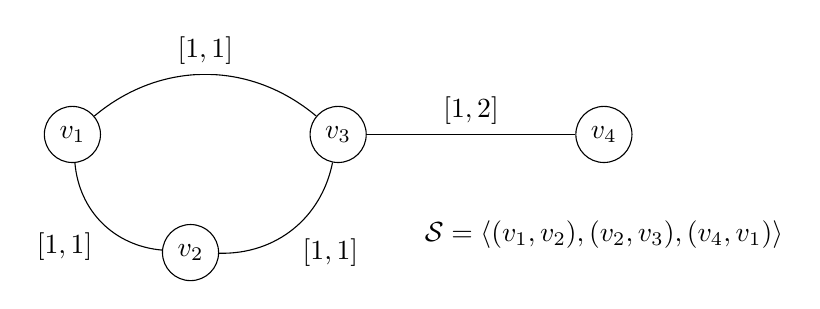
\begin{tikzpicture}[scale=0.75]
\tikzset{mapf-vertex/.style={circle, draw}}
\node[mapf-vertex] (v1) at (0.5, 0) {$v_1$};
\node[mapf-vertex] (v2) at (2.5, -2) {$v_2$};
\node[mapf-vertex] (v3) at (5, 0) {$v_3$};
\node[mapf-vertex] (v4) at (9.5, 0) {$v_4$};
\node at (9.5, -1.7) {$\sourcetargets = \tuple{(v_1, v_2), (v_2, v_3), (v_4, v_1)}$};

\draw (v1) to[bend right=40] node [below left,midway, fill=white] {$[1, 1]$} (v2);
\draw (v2) to[bend right=40] node [below right,midway, fill=white] {$[1, 1]$} (v3);
\draw (v3) to[bend right=40] node [above,midway, fill=white] {$[1, 1]$} (v1);
\draw (v3) to node [above,midway, fill=white] {$[1, 2]$} (v4);
\end{tikzpicture}
\caption{MAPF-TU with \emph{sensing} instance showing that replanning is not complete.
The initial and goal vertices of the three agents are indicated in the bottom right.
A policy-based solution consists in Agents 1 and 2 waiting for 2 time steps, then moving to their goal vertices, and Agent 3 moves immediately to $v_3$, then depending on the sense elapsed time, moves to its goal vertex or waits one time step and then moves.
}
\label{fig:replanning-incomplete}
\end{figure}


In Section~\ref{sensing}, we proposed an \emph{online} approach to consider agents' ability to sense their current location and time. 
An alternative approach is to consider the agents' ability to sense their location offline, i.e., when executing the solution. 
This means the planning algorithm will output an execution policy for each agent instead of a sequence of \emph{moves} and \emph{waits}. 
A policy may instruct the agent to perform different actions depending on the information it obtains via sensing. 
%
Considering sensing opportunities in this way can lead to significant cost reductions, compared to the replanning approach proposed in Section~\ref{sensing}. Some problems cannot be solved with the replanning approaches we proposed, but can be solved with a carefully crafted offline policy. 



Figure~\ref{fig:replanning-incomplete} illustrates an example of such an MAPF-TU problem instance. For this problem instance, there exists no safe, offline solution. This implies that we cannot perform online replanning. For safety, our current online approach begins by executing an offline solution and improves upon it.
% \shashank{The way we handle things online, I guess there is a solution to this problem although we cannot improve it using \emph{sensing}.
% The online approaches we address start from an initial offline, safe solution. In this case, CBSTU would give a solution like: Agt1 and Agt2 wait for 2 time units and Agt3 moves to v3, next they move to their target vertices at time three. We mention that agent can decide when to leave a vertex. Online: However, even if Agt3 senses that it is at v3 at time one, it cannot do anything just to ensure safety. If communication is allowed it will improve. For this example, whatever a pair of individual plans a joint policy tree would offer, can be generated by sensing+communication.}
%
However, creating offline policies for multi-agent problems can be extremely difficult, e.g., in models such as Decentralized-POMDP~\shortcite{bernstein2002complexity}. Developing efficient offine algorithms for MAPF-TU is left for future work. 




\subsection{Bounding Edge Traversal Time From Experience}
\label{sec:sample-complexity}
%[[Roni: here will come some theoretical analysis of how one can learn the bounds from experience and use them to do something useful. This is a work in progress with Brendan]]
The main assumption in a \mapftu problem is that the upper and lower bounds on edges' durations are given as input. While in some cases such information is given as input, 
% . 
% This is given in some cases, or may be estimated by analyzing the variance due to the agents' control. 
another approach is to \emph{learn} these upper and lower bounds from experience. 
 We describe here one way to do so. 


Consider a setting where the time it takes to traverse an edge $e$ is independent across executions and drawn from some unknown distribution $D_e$ of edge-traversal durations.  
For every edge $e$, we collect $M(e)$ samples $e_1,\ldots e_{M(e)}$ from $D_e$. 
Each sample is collected from a different execution, since multiple traversals of $e$ may be correlated with each other. Note, however, that we do assume that every traversal of $e$, taken in isolation, has the same distribution $D_e$. 
%\roni{Brendan, does this parse Ok?}

% Bounding a single edge
Let $L(e)=\min_{i\in\{1,\ldots,M(e)\}} e_i$ and $U(e)=\max_{i\in\{1,\ldots M(e)\}} e_i$ be the minimum and maximum observed duration it took to traverse $e$. 
The probability that the duration of a future traversal of $e$ will be outside the interval
$[L(e), U(e)]$ is given by the following theorem. 
\begin{theorem}
If $M(e)\geq \Omega(\frac{1}{\epsilon}\log\frac{1}{\delta})$, then with probability $1-\delta$ over the prior executions, the delay on edge $e$ lies in the interval $[L(e),U(e)]$ with probability $1-\epsilon$.
\label{simple-bound-thm}
\end{theorem}
In other words, if the number of samples $M(e)$ is at least $\Omega(\frac{1}{\epsilon}\log\frac{1}{\delta})$,  
then with probability higher than $1-\delta$ the $L$ and $U$ of our sample satisfies that 
the probability that traversing $e$ will take a duration not in $[L(e),U(e)]$ is smaller than $\epsilon$. 
The proof of Theorem~\ref{simple-bound-thm} is given in Appendix~\ref{appendix:sample-complexity}. 

% Bounding a solution
Now, consider a \mapftu instance in which we set the lower and upper bounds edge durations of every edge $e$ to be the observed lower and upper bounds $L(e)$ and $U(e)$, respectively. 
I.e., setting $w^{-}(e)$ and $w^{+}(e)$ to be $L(e)$ and $U(e)$. 
We call this \mapftu instance an \emph{empirical \mapftu instance}. 
We can use Theorem~\ref{simple-bound-thm} to upper bound on the probability that 
a solution to an empirical \mapftu instance will cause a collision. 
In other words, we can compute a lower bound to the probability that a solution to an empirical \mapftu instance is indeed safe w.r.t. the real world. 


To do so, we introduce some additional notation. 
Let $\Pi$ be a solution to an empirical \mapftu instance 
and let $E$ be the number of distinct edges in $\Pi$. 
For any $\delta'\in (0,1)$, let $\epsilon(e,\delta')$ be the minimum $\epsilon$ for which the bound of Theorem~\ref{simple-bound-thm} holds for the number of examples we possess for $e$ and $\delta$ set to $\delta'/E$. 
That is, 
\begin{equation}
    \epsilon(e)=O\left(\frac{1}{M(e)}\log\frac{E}{\delta'}\right)
\end{equation}

% is the minimum $\epsilon$ for which the bound of Theorem~\ref{simple-bound-thm} holds with $\delta'=\delta/E$ for the number of examples we possess for $e$. 


% the following state this formally, 

% To state Theorem X we define the following. 
% ... $\epsilon(e)$....
\begin{theorem}
Let $\Pi=\{\pi_1,\ldots,\pi_k\}$ be a solution to an empirical \mapftu problem. 
Then for $\delta, \epsilon>0$ with probability $1-\delta$ we obtain lower and upper bounds for every edge such that the probability that $\Pi$ can be safely executed is at least 
$1-\sum_{i=1}^k\sum_{e\in \pi_i} \epsilon(e)$. 
\label{the:solution-safe-prob}
\end{theorem}
\begin{proof}
$\Pi$ is a safe solution to the corresponding empirical \mapftu instance. 
Therefore, if executing $\Pi$ leads to a collision, then the duration of at least one move action in $\pi$ exceeded the lower or upper bound of the corresponding edge duration. Taking the union bound over all move actions of all agents, we obtain that the probability of this occurring is at most $\sum_{i=1}^k\sum_{e\in \pi_i} \epsilon(e)$. Hence the probability no collisions occur is as claimed.
% , it means there is an edge $e$ and a move action in $\Pi$ that traversed it, 
% such that the duration it 
% there exists at least one edge $e$ that is traversed in an action in a single-agent plan of one of the agents, such that  and the duration it will to traverse it w. 
% the duration of traversing at least one of the edges in the single-agent plan of at least one of the agents must have been 
% The probability that the edge duration of any of the traversals $t=1,\ldots,T$ of the $E$ edges is violated in an execution of the solution we produce is $1-\sum_{e\text{ is the }t^\text{th} \text{edge}}{\epsilon(e)}$ where $\epsilon(e)=O(\frac{1}{M(e)}\log\frac{E}{\delta})$ is the minimum $\epsilon$ for which the bound of Theorem~\ref{simple-bound-thm} holds with $\delta'=\delta/E$ for the number of examples we possess for $e$. 
% Thus we can obtain a probabilistic safety guarantee for the entire execution. In particular, since the guarantee for the final execution is a conditional probability statement, conditioned on the $E$ individual intervals being correct, we obtain that overall the probability, that the solution is actually safe, is at least $(1-\delta)(1-\sum_{e\text{ is the }{t^\text{th}} \text{ edge}}\epsilon(e))$. 
% We stress that the union bound does not require any assumptions of independence across edges during an execution. 
\end{proof}

% If the solution includes $E$ distinct edges and traverses $T$ edges in total, then we can take a union bound over the $T$ invocations of the bound in Theorem~\ref{simple-bound-thm} to obtain with probability $1-\delta$ over the data collected from past executions that all of the bounds are correct. Hence, the probability that the guarantee provided for any of the traversals $t=1,\ldots,T$ of the $E$ edges is violated in an execution of the solution we produce is $1-\sum_{e\text{ is the }t^\text{th} \text{edge}}{\epsilon(e)}$ where $\epsilon(e)=O(\frac{1}{M(e)}\log\frac{E}{\delta})$ is the minimum $\epsilon$ for which the bound of Theorem~\ref{simple-bound-thm} holds with $\delta'=\delta/E$ for the number of examples we possess for $e$. 
% Thus we can obtain a probabilistic safety guarantee for the entire execution. In particular, since the guarantee for the final execution is a conditional probability statement, conditioned on the $E$ individual intervals being correct, we obtain that overall the probability, that the solution is actually safe, is at least $(1-\delta)(1-\sum_{e\text{ is the }{t^\text{th}} \text{ edge}}\epsilon(e))$. 
% We stress that the union bound does not require any assumptions of independence across edges during an execution. 


The bound $[L(e),U(e)]$ is always valid for the given $\epsilon(e)$ we obtain as a function of $\delta$ and $M(e)$. 
However, if we are seeking a particular safety level, say some target $\epsilon'$ for each edge giving an overall bound that the solution is safe with probability $1-\epsilon$, then the bounds thus obtained may be too conservative. 
Eventually, especially with a large sample size, our examples will include ``outlier'' events that occur with probability far less than $\epsilon'$. Here is an alternative for large sample sizes that will allow us to approach an optimal interval $[L,U]$ for a given safety bound $1-\epsilon$.
\begin{theorem}\label{quantile-bound-thm}
For any $\alpha>1$, $\delta\in (0,1)$, and $\epsilon\in (0,1)$, let $[L(e),U(e)]$ be any interval containing at least $(1-\frac{\epsilon}{\alpha})M(e)$ examples for $e$ where $M(e)\geq \Omega(\frac{\alpha}{\epsilon(\alpha-1)^2}(\log\frac{\alpha}{\epsilon}+\log\frac{1}{\delta}))$. Then, with probability $1-\delta$ over prior executions, the delay for edge $e$ lies in the interval $[L(e),U(e)]$ with probability $1-\epsilon$.
\end{theorem}
The proof for Theorem~\ref{quantile-bound-thm} is also given in Appendix~\ref{sec:sample-complexity}. 
This theorem provides greater flexibility when constructing a \mapftu instance from empirical data, as one can take for every $e$ any interval in $[L(e),U(e)]$ that captures a sufficient number of samples. Then, one can use this more refined bound in Theorem~\ref{the:solution-safe-prob} to obtain a more refined bound on the safety of the generate plans. A deeper study of this is a topic of future work. 

% For this we will need the relative-error ``agnostic''/``non-realizable'' version of the VC-dimension bound \cite{li2001improved}, again stated in simplified form for our purposes\footnote{%
% In Li et al's statement, we actually put $\nu=2\epsilon$ and replace $\alpha$ by $\frac{\alpha-1}{4+(\alpha-1)}\geq \frac{\alpha-1}{4}$, so that if $r$ is the true error and $s<\epsilon$ is the empirical error, the obtained bound on $d_\nu(r,s)=\frac{|r-s|}{r+s+\nu}$ of $\frac{\alpha-1}{4+(\alpha-1)}$ implies $r<\alpha\epsilon$.}:
% \begin{theorem}[cf.~\cite{li2001improved}]\label{optimal-agnostic-vc-bound}
% Let $\mathcal{C}$ be a class of Boolean functions of VC-dimension $d$, let $\epsilon,\delta\in (0,1)$, and let $\alpha >1$. With probability $1-\delta$ every $c\in\mathcal{C}$ that is true at least a $(1-\epsilon)$ fraction of $m\geq \Omega(\frac{1}{\epsilon(\alpha-1)^2}(d\log\frac{1}{\epsilon}+\log\frac{1}{\delta}))$ examples satisfies $\Pr[c(x)=1]\geq 1-\alpha\epsilon$.
% \end{theorem}

% Theorem~\ref{quantile-bound-thm} is now immediate:
% \begin{proof}
% Again, the class of intervals has VC-dimension 2. Thus, by Theorem~\ref{optimal-agnostic-vc-bound} with $\epsilon$ set to $\epsilon/\alpha$, we see that if $M(e)\geq\Omega(\frac{\alpha}{\epsilon(\alpha-1)^2}(\log\frac{\alpha}{\epsilon}+\log\frac{1}{\delta}))$, every interval $[L,U]$ that is true of $(1-\frac{\epsilon}{\alpha})M(e)$ examples indeed satisfies $\Pr[e\in [L,U]]\geq 1-\alpha\frac{\epsilon}{\alpha}=1-\epsilon$.
% \end{proof}
% Note that we can make use of {\em any} $[L,U]$ that covers sufficiently many examples. 
% \roni{There are many options, e,g, improving the lower bound that we get from CBSTU}

% Some shortest such interval is a natural choice, or we might take $L$ to be the $\frac{\epsilon}{2\alpha}$ empirical quantile and $U$ to be the $(1-\frac{\epsilon}{2\alpha})$ empirical quantile (thus balancing the probability of violating the upper and lower bound). Again we can use a union bound and thus obtain that as long as we are producing a plan with at most $T$ traversals of at most $E$ distinct edges for which we have observed every edge in at least $\Omega(\frac{T\alpha}{\epsilon(\alpha-1)^2}\log\frac{E}{\delta})$ prior executions, the intervals are all correct with probability $1-\delta$, and hence the plan will execute safely with probability $(1-\delta)(1-\epsilon)$ overall.



% \begin{theorem}
% \label{the:safety}
% For a given graph network $G=(V,E)$, if we observed each edge $e \in E$ at least $m$ times then a solution obtained by the MAPF-TU framework using $L$ and $U$ bounds for individual $e$ is \emph{safe} with probability $P?$
% \begin{proof}
% \textcolor{red}{TODO}
% \end{proof}

% \end{theorem}



\section{Conclusion and Future Work}

In this paper, we studied the Multi-Agent Pathfinding with Time Uncertainty (\mapftu) problem, which is a Multi-Agent Pathfinding (MAPF) problem in which there is uncertainty over the time it takes an agent to traverse an edge. 
Specifically, for every edge we are given a lower and upper bound on the duration it takes to traverse it. 
%This type of uncertainty can be caused by different exogenous events, such as a human involving in an automated process. 
We focused on the problem of finding a \emph{safe} solution to a \mapftu instance, which is a solution that is guaranteed to avoid a conflict. 
To this end, we introduce the notion of \emph{potential presence} and \emph{potential conflicts}, where a solution is safe iff it has no potential conflicts. Then, we propose two algorithms, called \odatu and \cbstu, that find safe and optimal solutions to a \mapftu instance. 
We implemented these algorithms and compared them experimentally on a variety of settings and maps. The results show that on our benchmark set of instances \cbstu significantly outperforms \odatu in terms of success rate. 

Then, we considered two online replanning settings, \sense and \sensecom, where the agents have sensing or communicating capabilities while executing a solution. We demonstrate the potential benefit of online replanning in both settings, and propose online replanning algorithms that can improve the executed solution cost. We analyze these replanning algorithms theoretically, showing that using them is always advantageous. However, experimentally, we observed that signifcant benefit for replanning only appeared in the \sensecom when optimizing for the optimistic SOC. 
%We introduced such an online replanning mechanism and presented, experimentally, its benefits, i.e., resulting in a lower cost.  The proposed replanning algorithms take advantage of the sensed information, but they do not rely on sensing the future or the ability of other agents to sense.
% This limits their effectiveness but makes them more robust to sensing failures in future. \roni{Maybe move the last two sentences to the discussion or conclusion sections?} \shashank{Check the last two lines, do they fit?}


Finally, we discussed possible extensions to \mapftu. One such extension is to considering offline the possibility that the agents will sense new information and replan online.  
Another extension suggests a statistical analysis that allows extracting from observed data the lower and upper bound edge traversal times. 
Yes another extension is where there lower and upper bound also on wait actions, e.g., for cases where an agent is not allowed to stay too long in some locations. % Added for a reviwer.

There are many directions for future work. One can explore other objective functions to the \mapftu problem, such as minimizing the expected cost (assuming the traversal time distribution is known). Another direction is to adapt additional MAPF solvers to solve \mapftu, e.g., ICTS~\shortcite{sharon2013increasing}, 
EPEA*~\shortcite{goldenberg2014enhanced},
or M*~\shortcite{wagner2015subdimensional}. Finally, one may explore how to extend \mapftu to cases in which time is not discretized and the environment is continuous~\shortcite{AndreychukYAS19}, or when the bounds over the edge traversal durations change over time. % Last bit added for a reviewer


\acks{This research is partially funded by NSF award IIS-1908287 to Brendan Juba; 
and BSF grant \#2018684 and ISF grant \# 210/17 to Roni Stern.}

\appendix
\section{Sample Complexity Proofs}
\label{appendix:sample-complexity}

In this appendix, we provide formal proofs for the main Theorems in Section~\ref{sec:sample-complexity}.

\subsection{Proof for Theorem~\ref{simple-bound-thm}}
This confidence bound is an easy consequence of basic statistical learning theory. 
We recall the number of examples needed to fit a class of Boolean functions is determined by the {\em VC-dimension}~\shortcite{vc71} of that class:
\begin{definition}
A set of points of a domain $X$ is {\em shattered} by a class $\mathcal{C}$ of Boolean functions on $X$ if for every
Boolean labeling of the set, there is some $c\in\mathcal{C}$ that gives each point in the set the desired label. $\mathcal{C}$ is then said to have {\em VC-dimension} $d$ if the size of the largest set shattered by $\mathcal{C}$ contains $d$ points.
\end{definition}
The exact asymptotic dependence of the confidence $\delta$ and accuracy $\epsilon$ obtainable for classes of a given VC-dimension and a given number of examples was recently determined by Hanneke~\citeyear{hanneke2016optimal}. We state this in slightly simplified form for our purposes\footnote{%
We obtain this statement from the usual form by fixing the ``labels'' to be all $1$, since we are looking for a set that contains all of the examples seen so far.}:
\begin{theorem}[cf.~\shortcite{hanneke2016optimal}]\label{optimalvc-bound}
Let $\mathcal{C}$ be a class of Boolean functions of VC-dimension $d$. Then, for every $\delta,\epsilon\in (0,1)$, with probability $1-\delta$ every $c\in\mathcal{C}$ that is true on $\Omega(\frac{1}{\epsilon}(d+\log\frac{1}{\delta})$ examples independently drawn from a distribution $D$ on $X$ satisfies $\Pr_{x\in D}[c(x)=1]\geq 1-\epsilon$.
\end{theorem}
This bound is asymptotically optimal, but the constants hidden by the $\Omega$ are large. 
Other forms of this bound that feature an additional $\log\frac{1}{\epsilon}$ factor may give a better quantitative guarantee for the concrete values of $\epsilon$ that occur in practice.
%\roni{I don't understand the last sentence. 1) what constants are there here? it's in $\Omega(\cdot)$ terms, 2) why would adding a constant help? there is no algorithm here, it's "only" an analysis, no?}

Theorem~\ref{simple-bound-thm} is now an immediate consequence:
\begin{proof}
Recall that the set of intervals has VC-dimension 2: it is easy to verify that no set of three points on the real line can be shattered (either two are identical or we can label the max/min points $1$ and the middle point $0$). It then follows from Hanneke's bound (Theorem~\ref{optimalvc-bound}) that with probability $1-\delta$, any interval that contains $\Omega(\frac{1}{\epsilon}\log\frac{1}{\delta})$ examples drawn independently from some common distribution $D$ will contain further points drawn from $D$ with probability $1-\epsilon$. In particular, $[L,U]$ is such an interval.
\end{proof}


\subsection{Proof for Theorem~\ref{quantile-bound-thm}}
To prove this Theorem, we will need the relative-error ``agnostic''/``non-realizable'' version of the VC-dimension bound \shortcite{li2001improved}, again stated in simplified form for our purposes\footnote{%
In Li et al's statement, we actually put $\nu=2\epsilon$ and replace $\alpha$ by $\frac{\alpha-1}{4+(\alpha-1)}\geq \frac{\alpha-1}{4}$, so that if $r$ is the true error and $s<\epsilon$ is the empirical error, the obtained bound on $d_\nu(r,s)=\frac{|r-s|}{r+s+\nu}$ of $\frac{\alpha-1}{4+(\alpha-1)}$ implies $r<\alpha\epsilon$.}:
\begin{theorem}[cf.~\shortcite{li2001improved}]\label{optimal-agnostic-vc-bound}
Let $\mathcal{C}$ be a class of Boolean functions of VC-dimension $d$, let $\epsilon,\delta\in (0,1)$, and let $\alpha >1$. With probability $1-\delta$ every $c\in\mathcal{C}$ that is true at least a $(1-\epsilon)$ fraction of $m\geq \Omega(\frac{1}{\epsilon(\alpha-1)^2}(d\log\frac{1}{\epsilon}+\log\frac{1}{\delta}))$ examples satisfies $\Pr[c(x)=1]\geq 1-\alpha\epsilon$.
\end{theorem}

Theorem~\ref{quantile-bound-thm} is now immediate:
\begin{proof}
Again, the class of intervals has VC-dimension 2. Thus, by Theorem~\ref{optimal-agnostic-vc-bound} with $\epsilon$ set to $\epsilon/\alpha$, we see that if $M(e)\geq\Omega(\frac{\alpha}{\epsilon(\alpha-1)^2}(\log\frac{\alpha}{\epsilon}+\log\frac{1}{\delta}))$, every interval $[L,U]$ that is true of $(1-\frac{\epsilon}{\alpha})M(e)$ examples indeed satisfies $\Pr[e\in [L,U]]\geq 1-\alpha\frac{\epsilon}{\alpha}=1-\epsilon$.
\end{proof}



\section{Unsound Range Constraints for Edge Conflicts}
\label{appendix:edge-constraint}

The following example demonstrate that using a naive way to set range constraints to resolve a swapping conflict may lead to finding a suboptimal solution.   

\begin{figure}[ht]
\centering
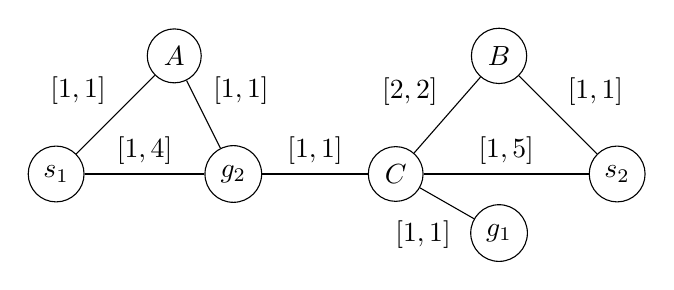
\begin{tikzpicture}[scale=0.75]
\tikzset{mapf-vertex/.style={circle, draw}}
\node[mapf-vertex] (s1) at (0, 0) {$s_1$};
\node[mapf-vertex] (a)  at (2, 2) {$A$};
\node[mapf-vertex] (t2)  at (3, 0) {$g_2$};
\node[mapf-vertex] (c)  at (5.75, 0) {$C$};
\node[mapf-vertex] (s2) at (9.5, 0) {$s_2$};
\node[mapf-vertex] (b)  at (7.5, 2) {$B$};
\node[mapf-vertex] (t1) at (7.5, -1) {$g_1$};
%\node[mapf-vertex] (t2) at (2, -2) {$v_2$};
% \node at (7.5, -1.4) {$\sourcetargets = \tuple{(s_1, g_1), (s_2, g_2)}$};

\draw (s1) -- (a) node [above left,midway] {$[1, 1]$};
\draw (s1) -- (t2) node [above,midway, fill=white] {$[1, 4]$};
\draw (a)  -- (t2) node [above right,midway, fill=white, fill opacity=1] {$[1, 1]$};
\draw (s2) -- (b) node [above right,midway, fill=white] {$[1, 1]$};
\draw (s2) -- (c) node [above,midway, fill=white] {$[1, 5]$};
\draw (b)  -- (c) node [above left,midway, fill=white] {$[2, 2]$};
\draw (c) -- (t1) node [below left,near end, fill=white] {$[1, 1]$};
\draw (c) -- (t2) node [above,midway, fill=white] {$[1, 1]$};
%\draw (c) -- (t2) node [below right,near end, fill=white] {$[1, 1]$};
\end{tikzpicture}
\caption{A \mapftu instance showing that using naive range constraints for edge-based conflicts in \cbstu leads to suboptimal solutions.
%The initial and goal vertices of the two agents are indicated in the bottom right.
}
\label{fig:no-range-conflicts-edges}
\end{figure}
\begin{example}
Consider the \mapftu instance depicted in Figure~\ref{fig:no-range-conflicts-edges}, 
and assume the objective is to minimize optimistic SOC. 
The initial solution 
\[
    \Big\{\big((s_1, g_2), (g_2, C), (C, g_1)\big),\big((s_2, C),(C, g_2)\big)\Big\}
\]
has a swapping conflict $\tuple{a_1,a_2,(g_2, C),[2,5]}$.
However, imposing the constraints that agent $a_1$ or agent $a_2$ cannot traverse the edge $(g_2, C)$ at any time step in $[2,5]$ rules outs all optimal solutions. Specifically, in all optimal solutions agent $a_1$ has the single-agent plan $\big((s_1,A), (A,g_2), (g_2, C) (C, g_1)\big)$ and agent $a_2$ has a single-agent plan in which $a_2$ arrives to $C$ at time step 4 and moves along $(g_2,C)$ immediately after. 
\end{example}


\vskip 0.2in
\bibliography{library}
\bibliographystyle{theapa}

\end{document}






